\documentclass[12pt]{report}
\usepackage[hidelinks]{hyperref}
\usepackage[T1]{fontenc}
\usepackage[utf8]{inputenc}
\usepackage[turkish,english,shorthands=:!]{babel}
\usepackage{apacite}
\usepackage[a4paper,left=41.2mm,top=25.2mm,right=24.2mm,bottom=35mm]{geometry} % left: 40mm, top: 25mm, right: 25mm, bottom: 25mm
\usepackage{epigraph}
\usepackage{graphicx}
\usepackage{float}
\usepackage[font={footnotesize,bf}]{caption}
\usepackage[font={footnotesize,bf}]{subcaption}
\usepackage{wrapfig}
\usepackage[usenames,dvipsnames]{color}
\usepackage[titletoc,title]{appendix}
\usepackage{afterpage}
\usepackage[doublespacing]{setspace}
\usepackage{tocloft}
\usepackage{url}
\usepackage{indentfirst}

% Turning off all figures, required for turnitin upload
% Remove the next two lines if you want the figures at their place
\usepackage[figuresonly,nolists,nomarkers]{endfloat}
\renewcommand{\processdelayedfloats}{}

% Same fonts for URL
\AtBeginDocument{\urlstyle{APACsame}}

% Figure and Table counters
\usepackage{chngcntr}
\counterwithout{figure}{chapter}
\counterwithout{table}{chapter}


%****************************************
% SPACING

% Footnote line spacing
\setlength{\footnotesep}{\baselineskip}

% Adding extra space between paragraphs
\setlength{\parskip}{0.5\baselineskip}
%........................................


%****************************************
% BIBLIOGRAPHY

% Bibliography line spacing
\usepackage{natbib}
\setlength{\bibsep}{0.0pt}

% Removing parentheses around year in bibliography
\AtBeginDocument{
\renewcommand{\BBOP}{}
\renewcommand{\BBCP}{}
}

% Adding ":" character before page number
\bibpunct[: ]{(}{)}{:}{a}{,}{~}
%........................................


%****************************************
% BLOCK QUOTES

% Spaces before and after block quotes
\usepackage{etoolbox}
\AtBeginEnvironment{quote}{\vspace{-\baselineskip}}
\AtEndEnvironment{quote}{\vspace{-\baselineskip}}

% Spaces before and after block quotes, indentation
\renewcommand{\quote}{\list{}{\rightmargin=4em\leftmargin=4em}\item\relax}

% Spacing
\expandafter\def\expandafter\quote\expandafter{\quote\singlespacing}
%........................................


%****************************************
% CHAPTERS

% Chapter titles
\usepackage{titlesec}
\titleformat{\chapter}[display]
        {\normalfont\fontsize{14pt}{14pt}\centering\bfseries}{\MakeUppercase{\chaptertitlename}\  \thechapter}{2\baselineskip}{\uppercase}
\titleformat*{\section}{\bfseries\fontsize{12pt}{12pt}}
\titleformat*{\subsection}{\bfseries\fontsize{12pt}{12pt}}

% Chapter title spacing
\titlespacing{\chapter}{0pt}{13mm}{3\baselineskip} % Centered, Top: 50mm, Next: 3 line after
% Bibliography title spacing
\titlespacing*{name=\chapter,numberless}{0pt}{16mm}{4\baselineskip} % Centered, Top: 50mm, Next: 4 line after

% RENAMING CHAPTER TITLES
\addto\captionsenglish{%
  \renewcommand{\contentsname}{\MakeUppercase{Table of Contents}}%
  \renewcommand{\listtablename}{\MakeUppercase{List of Tables}}%
  \renewcommand{\listfigurename}{\MakeUppercase{List of Figures}}%
  \renewcommand{\bibname}{\MakeUppercase{Select Bibliography}}%
}
%........................................


%****************************************
% EPIGRAPH

% Epigraph setup
\setlength{\epigraphwidth}{.65\textwidth}
\setlength{\epigraphrule}{0pt}
%........................................


% PDF setup
\hypersetup{
    pdftitle			= {MFA Thesis},
    pdfauthor			= {Mustafa ilhan},
    pdfsubject			= {Trash, Art},
    pdfkeywords			= {mfa thesis, trash, art},
    colorlinks			= false,
    pdfborder			= {0 0 0},
    pdfpagemode			= UseOutlines
}


% Utilities
\providecommand{\quotes}[1]{``#1''}
\providecommand{\singlequotes}[1]{`#1'}
\providecommand{\comment}[1]{\textcolor{cyan}{#1}}
\providecommand{\summary}[1]{\textcolor{blue}{[#1]}}
\providecommand{\paraphrase}[1]{\textcolor{magenta}{\quotes{#1}}}


%****************************************
% BEGIN
\begin{document}
\pagenumbering{gobble}
\selectlanguage{english}


%****************************************
% COVER
\begin{titlepage}
\singlespacing
    \begin{center}
        
        \vspace*{20mm}
        \uppercase{Transforming Trash as an Artistic Act}\\
        \vspace*{3\baselineskip}
        A Master’s Thesis\\
        \vspace*{3\baselineskip}
        by\\
        MUSTAFA İLHAN
        
        \vfill
        Department of\\
        Communication and Design\\
        İhsan Doğramacı Bilkent University\\
        Ankara\\
        January 2016
        \vspace*{28mm}
        
    \end{center}
\end{titlepage}
%........................................


%****************************************
% BLANK PAGE
\clearpage
\afterpage{\null\newpage}
\clearpage
%........................................


%****************************************
% DEDICATION
\newenvironment{dedication}
  {\clearpage           % we want a new page
   \thispagestyle{empty}% no header and footer
   \vspace*{2in}		% some space at the top 
   \centering
  }
  {\par					% end the paragraph
   \vfill
   \clearpage           % finish off the page
  }

\begin{dedication}
To my family and for those who embrace trash
\end{dedication}
%........................................

\pagenumbering{roman}

%****************************************
% TITLE PAGE
\clearpage
\thispagestyle{empty}
\singlespacing
	\begin{center}
        
        \vspace*{25mm}
        TRANSFORMING TRASH AS AN ARTISTIC ACT\\
        \vspace*{4\baselineskip}
        Graduate School of Economics and Social Sciences\\
        of\\
		İhsan Doğramacı Bilkent University\\
		\vspace*{2\baselineskip}
        by\\
       	\vspace*{2\baselineskip}
        MUSTAFA İLHAN\\
        \vspace*{3\baselineskip}
        In Partial Fulfilment of the Requirements for the Degree of\\
		MASTER OF FINE ARTS\\
        \vspace{\baselineskip}
        in\\
        \vspace{\baselineskip}
        THE DEPARTMENT OF\\
        COMMUNICATION AND DESIGN\\
       	İHSAN DOĞRAMACI BİLKENT UNIVERSITY\\
        ANKARA\\
        \vspace{\baselineskip}
        January 2016
        
	\end{center}
\clearpage
%........................................


%****************************************
% APPROVAL PAGE
\clearpage
\thispagestyle{empty}
%\singlespacing
%\doublespacing
\noindent I certify that I have read this thesis and have found that it is fully adequate, in scope and in quality, as a thesis for the degree of Master of Fine Arts in Media and Design.\\

\noindent---------------------------------\\
Assist. Prof. Dr. Ersan Ocak\\
Supervisor\\

\noindent I certify that I have read this thesis and have found that it is fully adequate, in scope and in quality, as a thesis for the degree of Master of Fine Arts in Media and Design.\\

\noindent---------------------------------\\
Prof. Dr. Mehmet Yılmaz\\
Examining Committee Member\\

\noindent I certify that I have read this thesis and have found that it is fully adequate, in scope and in quality, as a thesis for the degree of Master of Fine Arts in Media and Design.\\

\noindent---------------------------------\\
Instructor Ekin Kılıç\\
Examining Committee Member\\

\noindent Approval of the Graduate School of Economics and Social Sciences\\

\noindent---------------------------------\\
Prof. Dr. Halime Demirkan\\
Director\\

\clearpage
%........................................


%****************************************
% ENGLISH ABSTRACT
\thispagestyle{plain}
\phantomsection
\addcontentsline{toc}{chapter}{ABSTRACT}
\doublespacing
\begin{center}
	\vspace*{13mm} % Top: 50mm
	{\fontsize{14pt}{14pt}\selectfont \textbf{\MakeUppercase{Abstract}}}\\
    \vspace{\baselineskip}
    TRANSFORMING TRASH AS AN ARTISTIC ACT\\
    İlhan, Mustafa\\
    M.F.A., Department of Communication and Design\\
    Supervisor: Assist. Prof. Dr. Ersan Ocak\\
    \vspace{\baselineskip}
    January 2016
\end{center}
%\singlespacing
\par Usage of non-art objects in the artworks can be traced back to the beginning of 20th century. This approach has broken the existing rules and extended the language of art in an unprecedented way. After that point, trash has found a place in the work of artists.

The purpose of this study is to discuss usage of trash in the context of art. This thesis questions the role of art in the transformation of discarded items through the approaches and methods of artists who use discarded materials in their works. It examines why and how artists use discarded materials and how their artworks can be understood regarding theoretical and cultural aspects. This study is supported by theoretical and philosophical ideas about garbage.

Within this framework, thesis project argues that it is possible to see the process of transforming trash as an artistic act. In the scope of the project, discarded papers are collected with the help people and transformed to notebooks. Progress and collected materials are recorded on a website. Notebooks are installed in non-conventional art spaces such as library desks and computer labs that are frequently visited common places in order to invite people to use trash again. 

\noindent Keywords: Transformation of Trash, Trash in Art, Trash as an Art Material.
\clearpage
%........................................


%****************************************
% TURKISH ABSTRACT
\thispagestyle{plain}
\selectlanguage{turkish}
\phantomsection
\addcontentsline{toc}{chapter}{ÖZET}
\doublespacing
\begin{center}
	\vspace*{13.5mm} % Top: 50mm
	{\fontsize{14pt}{14pt}\selectfont \textbf{\MakeUppercase{Özet}}}\\
    \vspace{\baselineskip}
    \MakeUppercase{Sanatsal Bir Eylem Olarak Atığı Dönüştürme}\\
    İlhan, Mustafa\\
    Yüksek Lisans, İletişim ve Tasarım Bölümü\\
    Tez Yöneticisi: Yrd. Doç. Dr. Ersan Ocak\\
    \vspace{\baselineskip}
    Ocak 2016
\end{center}
%\singlespacing
\par Sanat işlerinde sanat dışı nesnenin kullanımı 20. yüzyılın başına kadar takip edilebilmektedir. Bu yaklaşım var olan kuralları yıkmış ve sanatın dilini eşi görülmemiş bir biçimde genişletmiştir. Bu noktadan sonra atık sanatçıların işlerinde yer bulmuştur.

Bu çalışmanın amacı sanatsal bağlamda atığın kullanımını tartışmaktır. Atık ürünlerin dönüştürülmesinde sanatın rolü, işlerinde atık maddeleri kullanan sanatçıların yaklaşımları ve yöntemleri üzerinden sorgulanmaktadır. Sanatçıların neden ve nasıl atık malzemeleri kullandıkları ve işlerinin kültürel ve kuramsal açılardan nasıl anlaşılabileceği araştırılmaktadır. Bu çalışma çöpe dair kuramsal ve felsefi fikirler ile desteklenmektedir.

Bu çerçevede, tez projesi atığı dönüştürme sürecinin bir sanatsal eylem olarak görülebileceğini savunmaktadır. Proje kapsamında atık kağıtlar insanların yardımıyla toplanıp not defterlerine dönüştürülmüştür. Süreç ve toplanan malzemeler bir web sitesinde kayıt altına alınmıştır. İnsanları atığı tekrar kullanmaya davet etmek amacıyla, defterler geleneksel sanat mekanı olarak kabul edilmeyen kütüphane, bilgisayar laboratuvarı gibi sık ziyaret edilen ortak kullanım alanlarına yerleştirilmiştir.

\noindent Anahtar Kelimeler: Atığın Dönüştürülmesi, Sanatta Atık, Sanatsal Malzeme olarak Atık.
\clearpage
%........................................

\selectlanguage{english}

%****************************************
% ACKNOWLEDGMENTS
\thispagestyle{plain}
\phantomsection
\addcontentsline{toc}{chapter}{ACKNOWLEDGMENTS}
\doublespacing
\begin{center}
	\vspace*{13mm}
	{\fontsize{14pt}{14pt}\selectfont \textbf{\MakeUppercase{ACKNOWLEDGMENTS}}}\\
    \vspace{3\baselineskip}
\end{center}
\par First and foremost, I would like to thank to my thesis supervisor Assist. Prof. Dr. Ersan Ocak for his endless patience, support and encouragement through the whole progress. He contributed in every way he can and guided me through the development of this thesis with his immense knowledge. I also would like to thank the rest of my thesis committee; Prof. Dr. Mehmet Yılmaz and Instructor Ekin Kılıç for their valuable contributions and insightful comments on the issues of this thesis.

I am grateful for Assist. Prof. Dr. Marek Brzozowski, Assist. Prof. Dr. Andreas Treske and Assist. Prof. Dr. Ahmet Gürata for their valuable ideas and criticisms.

I would like to thank my colleagues; Mert Aslan and Eda Erdem for their friendship and comments. 

I must thank to Melis Golar and Cemil Batur Gökçeer from Torun for opening their space to my project. 

I would like to thank my bosses and colleagues from Mobilus; Özgür Deniz Önür, Yağız Yaşaroğlu, Ekin Dino, Ayşegül Yaşaroğlu, Süleyman Yıldız and Aytaç Kocaman for their support, trust and collecting their discard for the thesis project.

I am grateful to M. Elgin Akpınar, Nihan Özdemirler, M. Cem B. Üstündağ, B. Ceren D. Üstündağ, Ayşenur Durgut, Emrah Şamdan, Duygu Ç. Şamdan, and Koray Benli for their valuable friendship, and also Ali from METU Technopolis İş Bank Office, Aykut from Modshifters, and Varuna Gezgin for collecting discarded materials for the thesis project.

Lastly and mostly, I would like to thank my family for their love, trust and support from the very beginning of this study. 
\clearpage
%........................................


%****************************************
% TABLE OF CONTENTS
\phantomsection
\addcontentsline{toc}{chapter}{TABLE OF CONTENTS}

\setcounter{secnumdepth}{3}
\setcounter{tocdepth}{3}

\renewcommand{\cftchapleader}{\cftdotfill{\cftdotsep}} % dots for chapters
\renewcommand{\cfttoctitlefont}{\MakeUppercase\hfil\bfseries\fontsize{14pt}{14pt}\selectfont}
\renewcommand\cftchapfont{\mdseries}
\renewcommand\cftchappagefont{\mdseries}
\renewcommand{\cftchappresnum}{CHAPTER\space}
\renewcommand{\cftchapaftersnum}{:}

\setlength{\cftbeforetoctitleskip}{20mm}
\setlength{\cftaftertoctitleskip}{3\baselineskip}
\setlength{\cftchapnumwidth}{7em}
%\addtolength{\cftchapnumwidth}{\cftchappresnum\cftchapaftersnum}

% Spacing between items
\setlength{\cftbeforesecskip}{\cftbeforechapskip}
\setlength{\cftbeforesubsecskip}{\cftbeforechapskip}

\begin{singlespace}
\tableofcontents
\end{singlespace}
\clearpage
%........................................


%****************************************
% LIST OF FIGURES
\phantomsection
\addcontentsline{toc}{chapter}{LIST OF FIGURES}

% Spacing between items
\makeatletter
\def\@chapter[#1]#2{\ifnum \c@secnumdepth >\m@ne
	\refstepcounter{chapter}%
	\typeout{\@chapapp\space\thechapter.}%
	\addcontentsline{toc}{chapter}%
	{\protect\numberline{\thechapter}#1}%
	\else
	\addcontentsline{toc}{chapter}{#1}%
	\fi
	\chaptermark{#1}%
	\if@twocolumn
	\@topnewpage[\@makechapterhead{#2}]%
	\else
	\@makechapterhead{#2}%
	\@afterheading
	\fi}
\makeatother

\renewcommand{\cftloftitlefont}{\MakeUppercase\hfil\bfseries\fontsize{14pt}{14pt}\selectfont}
\renewcommand{\cftfigaftersnum}{.}

\setlength{\cftbeforeloftitleskip}{20mm}
\setlength{\cftafterloftitleskip}{3\baselineskip}
\setlength{\cftbeforefigskip}{\cftbeforechapskip}

\begin{singlespace}
\listoffigures
\end{singlespace}
\clearpage
%........................................


%****************************************
% LIST OF TABLES
%\phantomsection
%\addcontentsline{toc}{chapter}{LIST OF TABLES}
%\listoftables
%........................................


\pagenumbering{arabic}


%****************************************
% CHAPTERS
\chapter{INTRODUCTION}



% Epigraph
\begin{singlespace}
\epigraph{One can even shout out through refuse \ldots}{\hfill---Kurt Schwitters, \textit{Kurt Schwitters}, 1985}
\end{singlespace}



According to dictionary Merriam-Webster, trash means anything useless, worthless or discarded. In parallel to this definition, the common perception is to get rid of them as soon as possible. People tend to think that trash is valueless because it is no longer needed or not wanted anymore. People want to get rid of them not thinking any alternative. Stav says that \quotes{[t]hey forget about it and don’t think about all the time and energy and money put into disposing of it} \citep[as cited in][]{navarro2015followingtrash}. On the other hand the issue of trash and transformation is not that simple. There are a lot of points to examine the trash.

% TODO Summarize
% Change in the production and consumption practices
\quotes{Over the course of the twentieth century, the twin developments of mass production and mass media in the capitalist economies of the Western Countries completed a total transformation of everyday life, reorienting almost every activity toward consumption. Things once locally produced and often handmade were now mass produced and commodified, turning local, artisanal producers into deskilled laborers serving the assembly line} \citep{pye2010trashculture}. As the result of it amount of goods boost and the cost of them significantly reduced. Things once reused again and again, now thrown away because it is more affordable to replace with new one. As the production increased its by-product material waste is also increased. \quotes{The phenomenon of waste comes clearly into focus not merely as a by-product of manufacturing processes, but rather as an integral element in cycles of production and consumption} \citep{pye2010trashculture}.

% Dominant approaches
During the last decades much attention has been devoted to the waste. In particularly environmental considerations dominates the perceptions of waste. \cite{ibarra2015beautiful} writes that \quotes{despite a relatively increased awareness about consumption and its consequences, the pace at which we also acquire and dispose of material objects is exploding}.

The act of trashing objects and the process of transforming them is not limited with geography, nationality and modern ages. It is a very common concept from developed cities to rural areas, from modern societies to ancient ones \citep[33]{rathje1992rubbish}. Anyone can encounter with trash in the crowded urban areas \quotes{as well as the remotest corners of the world} \citep[16]{cerny1996recycled}.

Trash is everywhere and, produced every time. It is inseparable from people's activities. \quotes{Every day, [people] put unwanted material in toilets and garbage bins, regularly flushing it away or taking it out in bags to be transported far away from} \citep[xxv]{zimring2012encyclopedia} their habitat. In other words, refuse is part of people's daily activities. Production of it never stops. Various activities of life such as eating, drinking, working and traveling leave behind wastes. These activities are not only taking place every time, but also spread to different places such as homes, offices and picnic areas. It is hard to say that any place is waste free. Nearly every place require waste bin because people can easily access vary kinds of goods that are going to be thrown away after used. If people do not find a waste bin, they often leave their trash wherever possible.

Trash is in the streets, in people's home, in the sea that people swim, rotating around the globe \footnote{Satellite discards are disposed to the atmosphere and they rotate around the globe like satellites.}. Even if trash is tried to move away from people's habitat, it is as close as the nearest waste bin.

People do not think what happens after they throw trash away.  It exits from people's life but not from the world. It is stacked to another place. A project conducted by MIT in America explores the journey of trash by placing trackers onto the trash \citep{chen2009mit}. According to their results trash spreads away across the country and this journey takes month. Further it is not limited with the border of America because they are exported to the other countries. In other words American's trash is not only their trash.

The vast amount of discarded items spread through the landfills to oceans. As commodities spread to the every corner of the world, trash do also. It moves from homes to garbage trucks, from streets to landfills and also from landfills to sculptures inside museums. In other words, trash is not only found on the most disgusting and avoided places, but also can be found on the most steril and frequently visited places.

% Different scales
The scale of trash production is not same for everybody or every country. \cite[2]{chen2015waste} writes that: 
\begin{quote}
The World Bank estimates that the amount of solid waste generated in cities is growing faster than the rate of urbanization. The higher the income level and the rate of urbanization, the greater the amount of solid waste produced. OECD\footnote{OECD (Organization for Economic Co-operation and Development) is an international economic organization of 34 countries. Turkey is a member of this organization.} countries produce almost half of the world’s waste. Africa and South Asia produce the least waste. High-income countries have the highest collection rates and are most likely to dispose of waste to landfills or incinerators. Low-income countries have the lowest collection rates and are most likely to dispose of their waste in open dumps. However, low-income countries also have the largest numbers of informal waste pickers who collect, sort, and reclaim recyclables---thus reducing costs to the city and to the environment.
\end{quote}

Similar to these as stated by \cite[16]{cerny1996recycled} \quotes{a person's wealth has become measured not only in how much he or she can afford to consume, but in how much he or she can afford to throw away.} Moreover from trash many unexpected results can be extracted. \cite[xxv]{zimring2012encyclopedia} argues that:
\begin{quote}
Our trash is a testament; what we throw away says much about our values, our habits, and our lives. ... Our trash is part of us, whether or not we choose to acknowledge it. ... The absence of a waste stream aroused suspicion, just as the presence of particular items tell us about the habits of the consumers who generate a waste stream.
\end{quote}

% Different types
Electronic waste, construction and demolition waste, medical waste are some of the various types of waste. They are result of different production and consumption practices. For example nuclear power generation and applications of nuclear fission or nuclear technology produces not only engery but also radioactive waste which is very dangerous for living creatures.

% Different diciplines
Trash attracts the attention of different peoples and disciplines \quotes{ranging from economics to environmental studies, but most particularly by those studying consumerism or material culture} \citep[63]{emgin2012trashion}. For instance for archaeologist dumps near the residential area are one of the significant places to figure out what people consume in the ancient times \citep{rathje1992rubbish}. Moreover scholars argues that there is a relationship between technological and waste. Trash can be seen as a design and technological problem \citep{mcdonough2010cradle}. Further economical aspect of trash can not ignored. \cite[65]{emgin2012trashion} states that there is a huge business based on eco-friendly products and recyclable goods that is increasingly promoted.

% Different people
Various people including garbage collectors and artists interact with trash for different purposes. There are people who collects plastics, scraps and papers from waste bins and landfills. For the ragpickers, collecting others excess and discard is significant source of economical income. They collect and clasify recycle materials to sell them. By collecting and selling them they endure their life. On the other side for some of the people it is not considered as trash. As stated by the editor of the Garbage issue of ReVista, Christmas decorations at Chocó, a poor region on Colombia’s Pacific Coast, are \quotes{all crafted from used tin cans, old newspapers, discarded textiles and found wood objects} \citep{erlick2015editorsletter}. She realized that any of them called the practice as recycling. For them using trash again and again is very natural and it is part of their life. On the contrary for the developed countries trash considered as a thing that must be avoided. There is no place for trash in their life. It can be understood from this anectode that approaches to the garbage are not same for all regions of the world. It can be said that \quotes{perceptions of waste and the value of material are neither static nor universally shared} \citep[xxvi]{zimring2012encyclopedia}.

As noted by \cite{pye2010trashculture} \quotes{at least since the early twentieth century, the concern with discarded things and materials has been a recurring theme in art}. In the beginning of the 20th century objects that are considered as art enter the scope of art making. Using non-art objects in the art opened new dimensions for the language of art and practice art making. This is a revolutionary change in the practice of art making. Production of art and the approach to the art changed dramatically. Picasso and Baraque are the first artists that used non-art object in their works. Later many of artists such as Kurt Schwitters and Joseph Cornell followed them with their collages and assemblages. Later Duchamp challenged the nature of art by using, non-unique, fabricated object to express his ideas. His work changed the way of perceiving art dramatically. With these developments trash has found a place in the art and contemporary artists become interested in trash. They use trash for different purposes and these are explored in detail in the following chapters. Trash find places in many mediums such as sculptures, paintings, assemblages and photographs. Artist express themselves through trash. Portraits are build from trash. Consumption habits of society are criticized through trash. \cite[2]{pye2010trashculture} states that \quotes{trash have influenced, and are also influenced by, cultural products such as films, visual art, museum exhibits and literature}.



%****************************************
\section{Purpose of the Study}
As it can be seen clearly that there are different aspects and approaches to the trash. In this thesis study to understand them is a key element because main driving force is to explore the alternative perceptions of trash. It is not static, not fixed, not totally isolated from people and social life. Instead of creating new usages, combinations or alternatives, common approach is to ignore all the possibilities embedded to the trash. People often do not look beyond the primary function of objects. To establish a solid understanding of trash and transformation of it, we have to give more attention to the trash. In order to move away the common perception this study asks that is it possible to reuse discarded items rather than refusing them?

The aim of this study is to explore the theories and methods focused on transformation of trash in the context of art and artistic act. Particularly this thesis is interested in the relationship between art and waste. It investigates that how waste represented as a subject and how waste is used as an art material to represent or draw attention to the other subjects. It asks and seeks answers of these questions: Why and how is trash used by the artist? Are there any differences with the original (or untouched, or blank) items compared to discarded (or used) items? Has using discarded material or trash have specific (or special) meaning (or message)?

Thesis project focuses on disposable items and specifically paper trash. Its purpose is to transform trash and make it worth to reconsider. At this point I need to state that the process of transformation is not to be confused with the kind of industrial recycling that is applying automated procedures to the products such as paper cups, glass bottles, plastics caps and aluminum cans with the purpose of returning them to the industrial production as raw materials. Further many people are inside the business of transforming trash through recycling and reusing. People has been looking for aluminum cans, glass bottles and plastics on the streets. They collect and sell them to survive. There are companies that are collect waste materials to regain them to the industry. In thesis they are not in the scope. Artist that give attention to the trash and transform them is in the scope of this thesis.

% TODO relocation.
% MOVE TO Conclusion of art chapter, discussion of transformation.
% FROM Trashion: The Return of the Disposed by Bahar Emgin
%\ People are often eager to see objects that were once considered useless and tasteless when they have been invigorated with new life.



%
%****************************************
\section{Structure of the Study}
Theory and artworks are not strictly separated from each other in this thesis. Artworks are explained with the help of theories. This study is structured by many examples of artworks in different part of the thesis. When an argument is presented, immediately an examplory artwork is given and how artists respond this issue is illustrated. Thereby artworks are examined in the theoretical and cultural context. Artworks are used as supportive elements for the stated arguments. However, artworks are discussed with all of their aspects. Only basic information is given and how it is related with this topic explained. By the way, it is better to keep in mind that all works can be analyzed in different contexts in more detail fashion.

Following chapter, Trash in Culture and Theory, explores the place of trash in the cultural life and theoretical approaches on trash. The aim is to understand the trash in cultural and theoretical aspects. Purpose is to establish better realization the notion of trash. This chapter provides theoretical and cultural background of the project. It is explored the trash is being worked is whose trash and what type of society generate this type of trash. What type of approach generate it and what are the dynamics of it? What type of trash we are talking about? It is understood through the patters of consumption patterns. And to reflect this cultural phenomena what philosophers and scholars say. Artist how they are reflected this notion.and also looked how scholars are conceptualized trash and its movement on the different values system. How can the transient nature of trash be explained?

In the third chapter, Trash (in) Art, seeks the root of usin discarded materials in the artworks and analyses the sample artworks and artists. As already artworks are mentioned in the different part of the thesis, in this chapter some of them analyzed deeply. Artists' methods and approaches to the subject are stated.

Fourth chapter consists of the overview of the project. In this chapter, my aim is to state the approach to subject clearly. The development process of the work is also presented in detail. Finally I put the factors, decisions and considerations that shaped the work.

The last chapter is reserved for an overall conclusion of this thesis and further suggestions on the subject and the project.



%****************************************
\section{A Note on Terminology}
Many scholars and authors have used broad range of terms to refer the notion. Garbage, trash, rubbish, debris, detritus, waste, scrap, junk, refuse, discard, disposal, litter are some of them. Sometimes these words are used to signify same concept. Although there are slight differences between these words. This situation signifies that literature of trash is so wide and there is no consensus on terminology. Words are used interchangeably. The book Rubbish: the Archeology of Garbage gives clearer definition of some these words:

\begin{quote}
Several words for the things we throw away ---\quotes{garbage}, \quotes{trash}, \quotes{refuse}, \quotes{rubbish}--- are used synonymously in causal speech but in fact have different meanings. \textit{Trash} refers specifically to discards that are at least theoretically \quotes{dry} ---newspapers, boxes, cans, and so on. \textit{Garbage} refers technically to wet discards--- food remains, yard waste, and offal. Refuse is an inclusive term for both the wet discards and the dry. Rubbish is even more inclusive: It refers to all refuse plus construction and demolition debris. The distinction between wet and dry garbage was important in the days when cities slopped garbage to pigs, and needed to have the wet material separated from the dry; it eventually became irrelevant, but may see a revival if the idea of composting food and yard waste catches on. We will frequently use "garbage" in this book to refer to the totality of human discards because it is the word used naturally in ordinary speech. The word is etymologically obscure, though it probably derives from Anglo-French, and its earliest associations have to do with working in the kitchen. \citep[9]{rathje1992rubbish}
\end{quote}

Artist Alice Bradshaw has published a \quotes{Rubbish Newspaper} which contains these words and shows their place in litreature and artworks. It is based on her extensive researh on this subject.

In addition to these there is also a confusion of the terms: reuse and recycling which are the general methods of transforming trash to the another object or concept. Both of them are used widely by scholars.

According to dictionary Merriam-Webster, the word reuse means \quotes{to use again especially in a different way or after reclaiming or reprocessing.} Reusing involves usage of the same product unchanged in form. Reusing lengthens the life of the item or material. The main purpose is to make the item last as long as it can. To reuse is to use something again instead of throwing it away. In this thesis, reuse is explored through the work of the artist.

On the other hand recycle means \quotes{to treat or process (used or waste materials) so as to make suitable for reuse.} In recycling an item, it is processed into a totally new product. Recycling occurs when waste in an unchanged chemical form is used in the same process that created the original product. Crushed glass containers used to make new glass containers, and scrap metal used in foundries can ge given as examples.

Recycling is very similar the rotting, and reuse is something like dry tree branches used by birds for their nest. These are two agents of nature to regain their resources.

Recycling can be viewed as down-cycling. The object smashed to the small particles to be used later in the production of something else. Although reuse can be viewed as up-cycling that gives another (or more) value to the discarded products. Down-cycling does not generates new meanings it tries to convert the product to already known state to process. 

\cite[72]{strasser1999waste} explains recycling by referring to the Oxford English Dictionary as:
\begin{quote}
... recycling originated in the oil industry during the 1920s, describing partially refined petroleum sent through the refining cycle again to reduce waste. Its use broadened during the 1960s, designating all kinds of reuse and reclamation, and the world became familiar during the early 1970s, as the burgeoning environmental movement promoted the separate collection of certain kinds of trash to promote their reuse in manufacturing.
\end{quote}

Some of the scholars use recycling \citep{cerny1996recycled,herman1998trashformations} for the recreation and transformation of waste. Many scholar used the word recycling when mentioning works use trash and the concept of it. However they are not mentioning the meaning that is decomposing things to the their particles. What they is actually is reusing and combining things, concepts, creating new mixtures. It is hard to say that they use it wrongly, but what they refer is actually upcycling. Creative reuse, inventing new things from discard. Upcycling is a term used by architect and designer William McDonaugh and chemist Michael Braungart and refers to \quotes{the process of converting an industrial nutrient (material) into something of similar or greater value, in its second life} \citep[as cited in][63]{emgin2012trashion}. It is argued that art, in this instance, acts as a tool of transformation and reintroduces into certain orders what was once deemed waste. This theory counters the argument that an object is dead once it is disposed of \citep{emgin2012trashion}. Some of the scholars and artist uses upcycling for their process. This thesis project is about those objects that are recreated from trash through the process of upcycling.





\chapter{TRASH IN CULTURE AND THEORY}



\begin{singlespace}
\epigraph{Anger is nothing compared to garbage:\\Garbage eats anger for breakfast.\\It eats all of us in the end.}{\hfill---Priscilla Uppal, \quotes{Uncle Fernando’s Garbage Triptych}}
\end{singlespace}



In this chapter trash and the practice of transforming it is examined in theoretical and conceptual aspect. Referred to the ideas of philosophers and anthropologists to establish a better understanding of trash beyond common perception and dictionary meaning of it.

Firstly, I focused on the disposable items that are designed to be ended up in waste bin after a single use. Their usage and place are examined in the society and how other artists used and transformed them is analyzed. Further, disposable items are one of the key material used in the thesis project. Therefore, they need to be discussed in detail. Secondly, I looked through the Žižek’s comments on ecological perspectives that dominate the approaches on rubbish. Lastly, through \textit{Rubbish Theory} transformation of trash and its various states as an object category is examined.



%****************************************
\section{Throwaway Culture}

Life Magazine (1955: 43) published an article titled \quotes{Throwaway Living} and proclaimed the arrival of the \quotes{throwaway society}. It is described as behavioral consumption pattern of society based on throwing away objects after use. The article addresses the question of \quotes{why [to] spend valuable time washing and reusing household objects like plates and silverware when they can be inexpensively made of plastic and disposed of after use?} \citep{tully2014throw}. One can claim that disposable items provide easiness by bringing affordable alternatives of daily used gadgets. With these items people can spend their time and effort for other activities. In fact, the term \quotes{throwaway society} is a critic of it by mentioning its wastefulness and has a slightly negative connotation.

According to findings of archaeologist Daniel Ingersoll the age of the throwaway world began not in the twentieth century but during the nineteenth century \citep[as cited in][41]{rathje1992rubbish}. On the other hand, scholars have criticized the notion of \quotes{throwaway society} as being insufficient and over generalization of consumer behavior \citep{gregson2007identity}. According to the result of their qualitative research on consumers over two-year, people are not as wasteful as claimed when considering household possessions such as television, furniture and toys. However, their research did not include disposable packaging and bottles. Therefore, the act of throwing away can be narrowed down to the specific goods.

In this thesis dealt specifically with industrially produced consumer discards and their subsequent transformation. This thesis is necessarily situated at a particular time, place, and sensibility: the consumer culture of the post industrial age. In its most basic form, consumer culture can be explained, as \quotes{the activities and ethics of a society are determined by patterns of consumption} \citep[2]{mamiya1992pop} rather than production.

% Disposable Items
Disposable items are made to be thrown away after used once or only a few times. They are not permanent or durable and not designed to be reused again. Packages of beverages, paper cups and tissues are some of them. They are used very short-time. Their lifetime can be measured in minutes in terms of usage. Although, their usage duration is very short, they continue to exist in nature.

Many products that are delivered in these days are not designed to last for a long time. As a result, this encourages people to continue throwing goods away instead of repairing and reusing them.

\citet[9]{hawkins2001plastic} argues that \quotes{Mass production of objects and their consumption depends on widespread acceptance of, even pleasure in, exchangeability; replacing the old, the broken, the out of fashion with the new. The capacity for serial replacement is also the capacity to throwaway without concern.} It can be understood that both mass production and consumption support each other. Not only consumerism, but also mass production plays significant role in this phenomena. They need to be considered as a whole.

The remarkable thing about many of these objects ---especially those produced in the last of the twentieth century--- is that they were specifically designed to end up on the garbage heap \citep{cerny1996recycled}. They were designed to decrease in value over time to be used one, or twice and then to be thrown away. This applies not only packing ---designed containers that protect and promote products--- but to an ever expanding list of products. \quotes{When an object is discarded, it is perceived as being no longer of value to the person or society that once possessed it. Once a newspaper is read, or a bottle of coca cola consumed, its basic function is fulfilled, and it is intended to be thrown out as trash} \citep{cerny1996recycled}.

% Being wasteful
As stated, \quotes{being wasteful in the ways [people] live is encouraged, expected and in many instances impossible to avoid} \citep[viii]{hawkins2005ethics} because the cost of repairing objects sometimes is higher than the original one or very close to it. On the other side, it is refused to use because of they are old fashioned even if they are perfectly fine. Moreover over time particularly electrical gadgets become incompatible with new formats and contents.

Technological advancements can be one of the factors that cause over-consumption habits. Disposable items with the help of industrialization can be produced easily with low cost and they reduce the labor and human resources as compared to the traditional ways. For instance, consider handkerchief versus napkin, glass versus paper cup. Another point is that they are more affordable regarding supply chain and cost. In other words, people can put new one easily after disposing it. Therefore, there is no need to save the old one. The last but not least increasing attention of hygiene is contributed to the extension of disposables in the market highly. \quotes{The commodities of food and drink must be safe, sterile and private} \citep[70]{kennedy2007ontology}.

%At the same time, thinkers such as Zygmunt Bauman and Giorgio Agamben have shed light on the fate of the human being as a wasted or discarded element in discourses of socio-political hygiene \citep{pye2010trashculture}.

\cite{kennedy2007ontology} notes that the germ theory prohibits companionship. The Latin root of this word, \textit{cum pani}, exactly means to share bread. However, insofar as each eater harbors untold numbers of hazardous germs, it is safest to keep one’s food strictly to one’s self. Safety in a world of bacteria implies isolation. Packaging goods successfully isolates both food and consumer within a structure of sterile control. In essence, it encloses the commons.

\citep[176--177]{strasser1999waste} narrates part of the history of this enclosure through the career of the disposable drinking cup, which appeared in the early years of the twentieth century:

\begin{quote}
While the sanitary advantages of toilet paper might have been obvious, those of the paper cup required a belief in germs. The widespread use of paper cups was a direct result of a public health crusade educating people about the invisible organisms spread by the common drinking cups once standard in public places, especially trains and railroad stations. Manufacturers of paper cups teamed up with public health authorities to campaign for federal and state regulations banning common drinking cups from use in interstate traffic. Succeeding in 1912, they competed for the business of the railroads and train stations\ldots 

Disposable paper cups met significant resistance. Most public places offered them in coin-operated dispensers, and some people were not willing to pay for what had once been free. Respectable travelers carried their own cups, available in metal and celluloid in a variety of collapsible and folding designs. Others reused paper cups from the trash or drank out of the public tanks, putting their lips to the faucet or using the cover of the tank as a cup. Some people protested against the vending machines: soldiers smashed paper cup dispensers in Washington’s Union Station during President Wilson’s inauguration in 1913. And some public places installed drinking fountains instead of paper cups dispensers, although at first these, too, were attacked as unsanitary because people could touch the nozzle with their lips.
\end{quote}

%\summary{Dark side} 
Nowadays usage of disposable items in the society is very widespread. As stated previously for same cases it is inevitable. Beyond the advantages of disposable items, there are dark sides of consuming them excessively. They result in mountains of garbage, spread through remotest corner of the world.

Handling of mountains of garbage is another subject and will not be discussed in this thesis. It is not claimed that whether usage of disposals is supported or not. It might be subject to another thesis. What is important here understanding the place of garbage for the people and the reflection (approach) of the artist. 



% Art
Some of the works of the artist can be examined in the light of discussed phenomena. They establish some methods to reflect the throwaway culture and its waste generated patterns. They offer new dimensions to see the subject.

% ARTWORK
% Portraits of Global Mass culture
\begin{figure}[h!]
\begin{subfigure}{.48\textwidth}
  \centering
  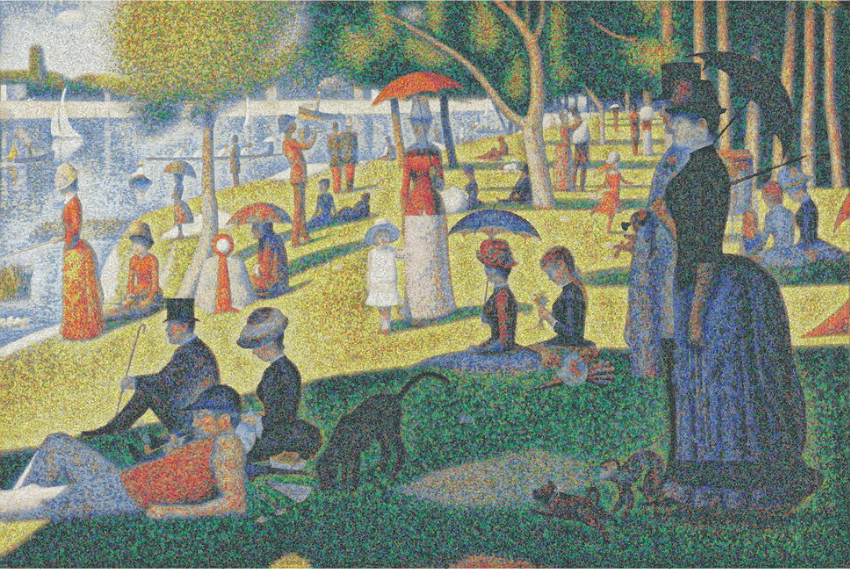
\includegraphics[width=\linewidth]{graphics/ChrisJordan_Numbers_OriginalView.jpg}
  \caption{Original view}
  \label{fig:ChrisJordan_Numbers_OriginalView}
\end{subfigure}
\hfill
\begin{subfigure}{.48\textwidth}
  \centering
  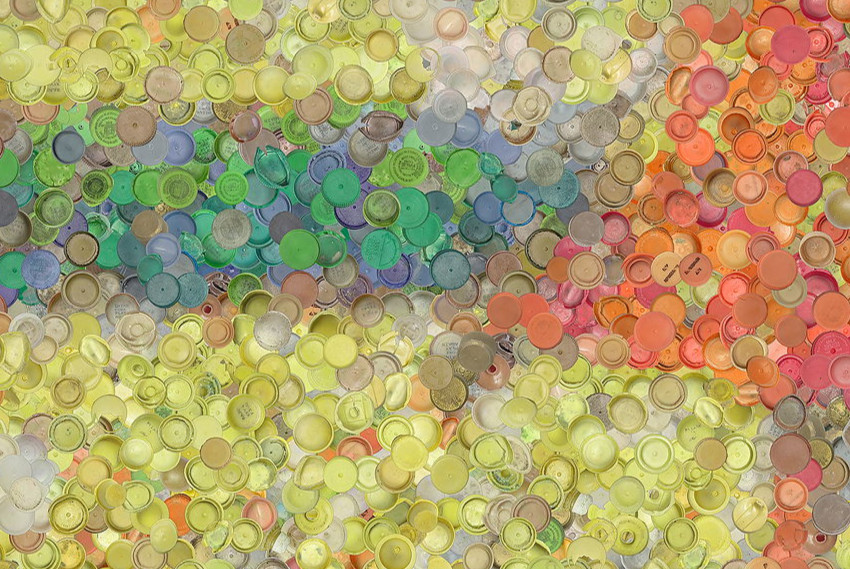
\includegraphics[width=\linewidth]{graphics/ChrisJordan_Numbers_CloseView.jpg}
  \caption{Close view}
  \label{fig:ChrisJordan_Numbers_CloseView}
\end{subfigure}
\caption{Chris Jordan, \textit{Caps Seurat}, 2011, Digital pigment print, 60x90" in one panel, and 88x132" in 3 panels}
\label{fig:ChrisJordan_Numbers_CapsSeurat}
\end{figure}

Chris Jordan creates digital photographic series that turns numbers to visuals. He provides a different way to understand the statistics and the reality behind the consumerism. He creates gigantic prints to express the numbers in a visual manner. He draws attention the global consumerism. His work reveals the reality that is hard to capture because of widespread acceptance among the community.

\textit{Caps Seurat} shown in figure \ref{fig:ChrisJordan_Numbers_CapsSeurat} displays four hundred thousand plastic bottle caps all together. \quotes{It equal[s] to the average number of plastic bottles consumed in the United States in every minute} says Jordan. It is one of the piece of Portraits of Global Mass Culture by photographer Chris Jordan. In this series, he revisits the statistics of modern societies. \cite{boustead2015impossible} explains that \quotes{Chris Jordan attempts to convey the vastness of modern consumption by breaking down annual statistics into more graspable quantities depicted by clever visualizations made of individual objects or groups of objects that he photographs.} Jordan says that \quotes{[t]here’s a disconnect that happens when we assume we know what we’re talking about when we talk about hundreds of millions of plastic bottles} \citep[as cite in][]{boustead2015impossible}. He argues that \quotes{translating these numbers from the deadening language of statistics into a visual language that allows some kind of comprehension} \citep[as cite in][]{boustead2015impossible}. He creates these works through the combining photographic illustration of everyday trash and mass consumption leftover. He draws attention to the blind unawareness entangled in consumerism. His work, while often disturbing, is a strong message about ignorant practices in people’s everyday lives, leaving it to the viewer to draw conclusions about the unavoidable consequences which will originate from people’s daily consumption routines. He recreates the most remarkable artworks with combining bits of trashes as a mosaic. Here he draws attention to the our consumerism and express them in visuals and all the material that we have in these days is trash to create this pictures.

%\summary{Analysis}
In fact, the work of Chris Jordan is a reproduction of \textit{A Sunday Afternoon on the Island of La Grande Jatte} which is one of the most notable works of Georges Seurat who was acknowledged as the painter of a post form of Impressionism called Neo-Impressionism. The work accepted as a well-known example of pointilizm that is a technique of painting in which little and individual dots of color are applied in patterns to construct an image. This method shows similarities with mosaics of ancient times and pixels of modern times. To make an work from bottle cups with different colors can be related to painting millions of small dots on a canvas. The shape of plastics cups similar to the dots painted onto the canvas so that there could not be a better example of reproduction.

Seurat spent over two years painting \textit{A Sunday Afternoon}, focusing meticulously on the landscape of the park. However, in our age, it takes only one minute to create the bottle caps that form this painting. In this respect, it reveals the point where society reached.

Visuals of Chris Jordan are like post-modern versions of mosaics. In the age of mass production and consumption, the most readily available material is trash. It is free and available everywhere, produced every time. Trash has different colors, sizes, and shapes. Therefore, it is a perfect material to build images from them. There is a great diversity of rubbish and offers new alternatives. Nothing is missing with the physical attributes of trash to create visual work.

% ARTWORK
% TEA BAGS
\begin{figure}[h!]
  \centering
  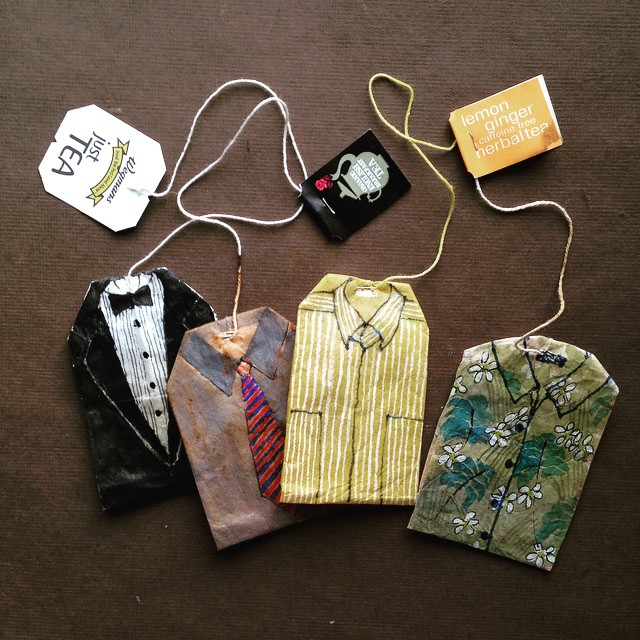
\includegraphics[height=6cm]{graphics/rubysilvious-teabag-Day169.jpg}
  \caption{Ruby Silvious, \textit{Day 169, 363 Days of Tea}, 2015, Mixed media on upcycled paper tea bags, Dimensions variable}
  \label{fig:RubySilvious_TeaBag}
\end{figure}
  
Visual artist and graphic designer Ruby Silvious embarked on a quirky, personal experiment, set to last for 363 days. She decided to re-purpose mushy and muddy tea bags as unconventional, blank canvases, just waiting to be filled with her artistic expression. The project, entitled \textit{363 Days of Tea}, allows Silvious to challenge herself by transforming the recycled material with her intricate illustrations. The artist draws, paints, and forms collages on the salvaged tea bags. This project serves as Silvious’ daily journal, allowing her to record her thoughts and feelings by creating wonderful moody and whimsical designs on little teabag papers. Every day she creates a new piece that reflects her impressions in that moment. Endeavour of re-purposing recycled and found materials. 

Work shown in figure \ref{fig:RubySilvious_TeaBag} is for fathers day. Works of Silvious catch the important moments of days and can be as a diary (or a record of that moment and day). Trashes transformed to diaries. Trash is everywhere, already at hand. Small pieces of paper or packages are used as a canvas. 

% ARTWORK
% COFFEE CUP
\begin{figure}[h!]
\begin{subfigure}{.48\textwidth}
  \centering
  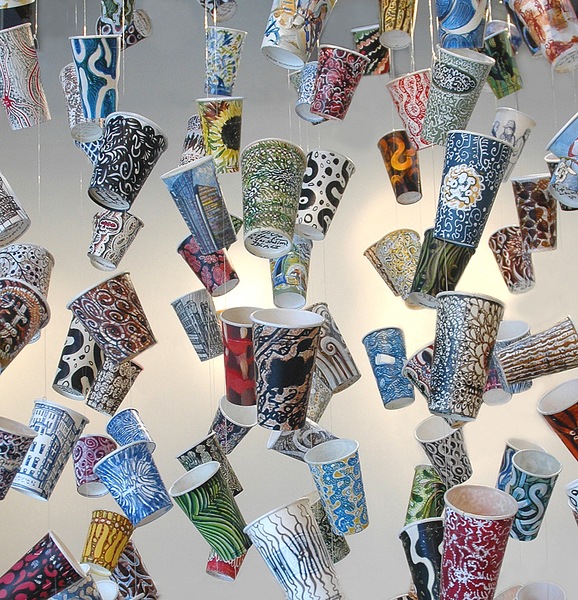
\includegraphics[width=\linewidth]{graphics/Gwyneth-Leech-cup5.jpg}
  \caption{Installation view}
  \label{fig:GwynethLeech_Installation}
\end{subfigure}
\hfill
\begin{subfigure}{.48\textwidth}
  \centering
  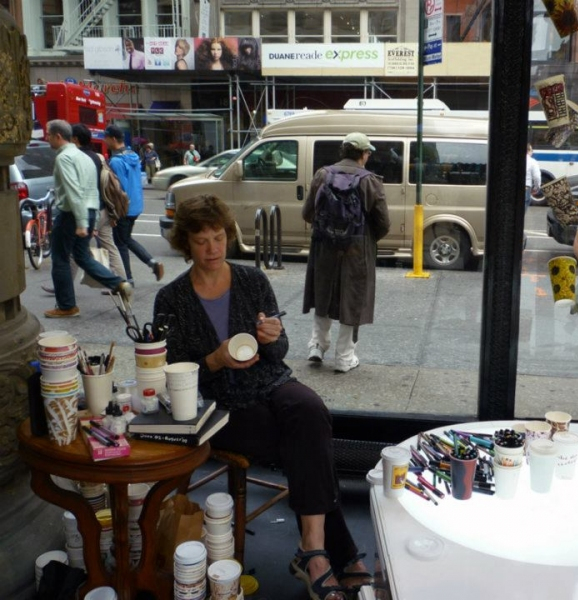
\includegraphics[width=\linewidth]{graphics/Gwyneth-Leech-cup3.jpg}
  \caption{Painting in the public}
  \label{fig:GwynethLeech_Public}
\end{subfigure}
\caption{Gwyneth Leech, \textit{365 A Year in Cups}, 2013, Mixed media on upcycled paper cups, Dimensions variable}
\label{fig:GwynethLeech_CoffeeCups}
\end{figure}

Gwyneth Leech saves all of her coffee cups to use them as canvases for her abstract illustrations. She transforms her coffee cups that are no longer junk but a tool for art, ideas, conversation, and memories of a social moment upcycled from the detritus of throwaway caffeine culture. Buying a beverage from a coffee shop is a daily event for Leech and also for many other people. These coffee shops are located all around the world and busy corners of cities. She uses cups as a canvas on which to draw and paint. Moreover, on the bottom of each one, she records the date, location, occasion and drink consumed so that every hand-made cup artwork becomes the record of a moment. The installation shown in figure \ref{fig:GwynethLeech_CoffeeCups} makes visible widely ignorant patterns of consumption; this is what one simple take-away beverage looks like over the course of many years, this is what would usually be thrown away. It can be seen as a measure of time gone by, of money spent, of volume to be taken up in a dump site. However, as \cite{leech2015cups} \quotes{upcycles each used cup into an artwork, it becomes the measure of other things as well: an artist’s regular habit of generating new ideas, a diary of time spent with friends and colleagues, and the cumulative positive effect of doing something small and manageable every day.} There are different versions of installations. Here paintings on paper coffee cups are displayed in an open window space and she publicly paints them. Her public drawing project were showed at many places and date. During public drawing projects, she draws with other people. She is inside of glass window not white, isolated cube. Glass window provide her to be close to public space. As she drinks her coffee publicly, and also paints them publicly. There is no difference between them, and also they should not be separated. By showing her practice publicly, she encourages other people in order to reconsider trash as a resource to make something. Further she is not only transforming her trash, it is every body’s trash because of everyone uses it.

These three artists mentioned here use disposable items to make their art. Their approach bring another dimension to criticize (or see) the disposable items. As it can be seen that new things can be built from them and they can be used for new purposes.

Throw away culture has a significant place in producing trash. It is a behavioral pattern, and an approach to objects and commodities. Some artists and people develop different approaches to them. In this type of culture or behavior throwing them is a natural act and promoted. Consumption and wasting things are encouraged. On the other hand, there are examples of saving everything instead of wasting. In the work of Song Dong, \textit{Waste Not}, thousands of domestic objects are exhibited. They are owned by his mother and saved for later use. They are extracted from her home. The compiled objects ranging from toothpaste to shoe, from bottles to toys. His mother lived a great depression in China, and suffered from poorness. As a result of it she developed the habit of saving things. After died of her husband this habit reached to extreme levels. She started to save every tiny object. For her, trash becomes an essential part of her life. In fact, it not is hard to say that preserved these things are not useless or worthless. She establishes a different relationship with these used objects.

Trash is much more than what people want to discard. Characteristic of people and societies can be understood from their produced trash. Trash can be seen as a reminder of consumption and production activities. In other words, trash is bound to them, and every different of them leaves a diverse range of trash that exposes its type of action. Trash tells about societies’ choices. What is being left is one of the key things to realize what kind of people, society, action produce it. At one side trash is a produced thing and what people consume is tells many things about them such as their choices, possessions. As scholars mentioned that throughout the discards of someone else many things can be understood. They are end product of people activities, and it can be traced through the discard and garbage. It is a great example of the approach to the trash is relative and changes from people to people.

% FROM drink UP, author: Werthan, Sarah, artist: Leech, Gwyneth. A Year in Cups. http://gwynethleech.com/
% trash and art collided. Paper and art, actually paper already medium of art, but is there anything different here. Itself is a part of a work, not the drawing, or painting.
% Documenting via a blog or a website. (what type of dimension it brings the work? maybe connect them, leave message.)
% Creating art in public places can demystify the process for passers by, Leech says, making artistic expression more accessible and part of people’s everyday lives. The reason of website.
% “People see that an artist can make work anywhere, and make creative spaces anywhere,” she asserts. 

\begin{figure}[h!]
  \centering
  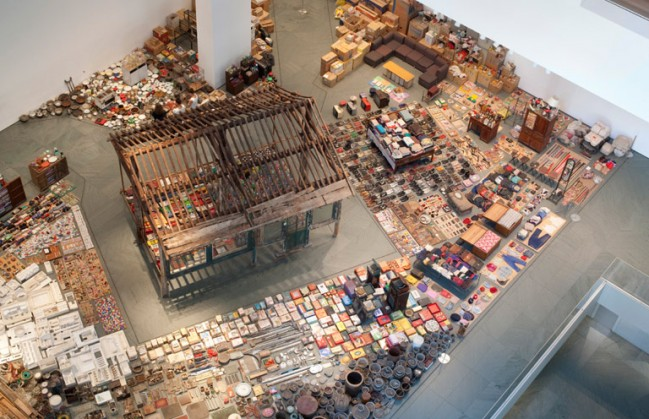
\includegraphics[height=8cm]{graphics/SongDong_WasteNot.jpg}
  \caption{Song Dong, \textit{Waste Not}, 1990}
  \label{fig:SongDong_WasteNot}
\end{figure}

Figure \ref{fig:SongDong_WasteNot} displays over ten thousand objects owned by Chinese artist Song Dong’s mother. She declined to discard anything if she could in some way reuse it. \textit{Waste Not} is an installation exhibited various museums of the world. This work can be seen as a work of collaboration of artist and his mother.

Song’s mother, Zhao Xiangyuan (1938–2009), was typical person of the generation of Chinese who lived through the poverty of the Cultural Revolution in the third quarter of twentieth century by the saying \textit{wu jin qi yong} (waste not). As a result, all commodities owned or collected items are stockpiled and preserved as protection against for future poverty, even in the times of improving economic conditions.

In the same way as other Chinese at the time, Zhao developed the habits of frugality and thrift in order to make the best of what limited she had. By recalling memories from childhood, Song says that \quotes{my mother always brought scraps of fabric to make clothes, because they did not need to be purchased with the government ---distributed clothing coupons.} She continued to collect them even in prosperity times because she feared that the shortages might some day return. The habit of waste not is seen as a \textit{fabao} ---literally a powerful weapon to protect against a return to hardships.

When Song’s father died suddenly in 2002 his mother suffered from loneliness and an emotional collapse. As a result of it her practice of saving matters was reached to extreme levels. Every possible space of her tiny house completely filled with thousands of domestic items. Song Dong and his sister Song Hui attempted to tidy up for her, but this led to conflict, as Zhao resisted their efforts to dispose of things that she saw as potentially useful. In other words, she maintained her habit. Song eventually realized that, as he states that \quotes{my mother’s need to fill space with daily-life objects resulted from a need to fill the emptiness after my father’s death.} He recognizes that \quotes{a person could live through several different lives in just one lifetime. In the wink of an eye, ones life could undergo great changes causing deep divisions between old and young.}

Everything that are exhibited in this work is different than presented on supermarkets. They are not new and not for sale. They represent a way of life. It is common a notion that the exhibitions of famous people’s possessions but this work is separated from them as showing ordinary people’s objects.

For most of people living in western modern societies it is unimaginable to live with all of these items together. However, for Chinese who are faced with same struggles share the same emotion and comment as \quotes{It’s not [only] your home, it’s [our] home.}

Jane Alison, senior curator at the Barbican Art Gallery in London, states that \quotes{\textit{Waste Not} helps us to understand the reality of Chinese history and culture in the twentieth century in a way that newspapers can’t} \citep[as cited in][]{needham2015chinese}



As it can be understood trash reflects people’s habits. It is like a mirror. It can not be separated from their producers and it is well studied area by scholars. Garbology is a study of waste as a social science. It applies methodologies of archeology to the human debris. Weberman infamously used techniques of what he deemed garbology to uncover what he saw as the essential nature of people. He once said, perhaps indirectly referencing Jean Brillat-Savarin’s quote about food, \quotes{You are what you throwaway} \citep[as cited in][301]{lukas2012garbage}. The field of garbology involves the study of refuse and waste. It enables researchers to document information on the dump and changing patterns of modern rubbish, hence assisting in the study of contemporary human society or culture \citep{roy2012garbology}. According to the Oxford English Dictionary, the term was first used by waste collectors in the 1960s. Weberman popularized the term in describing his study of Bob Dylan’s garbage in 1970. It was pioneered as an academic discipline by William Rathje at the University of Arizona in 1973. The work of archaeologists such as William Rathje and Cullen Murphy has offered significant insights into the relationship between archaeological artifacts and garbage, exploring the function of trash as a resource for understanding the cultural and social practice. With the help of mentioned understanding of trash, what can be understand from the works of art?

\begin{figure}[h!]
  \centering
  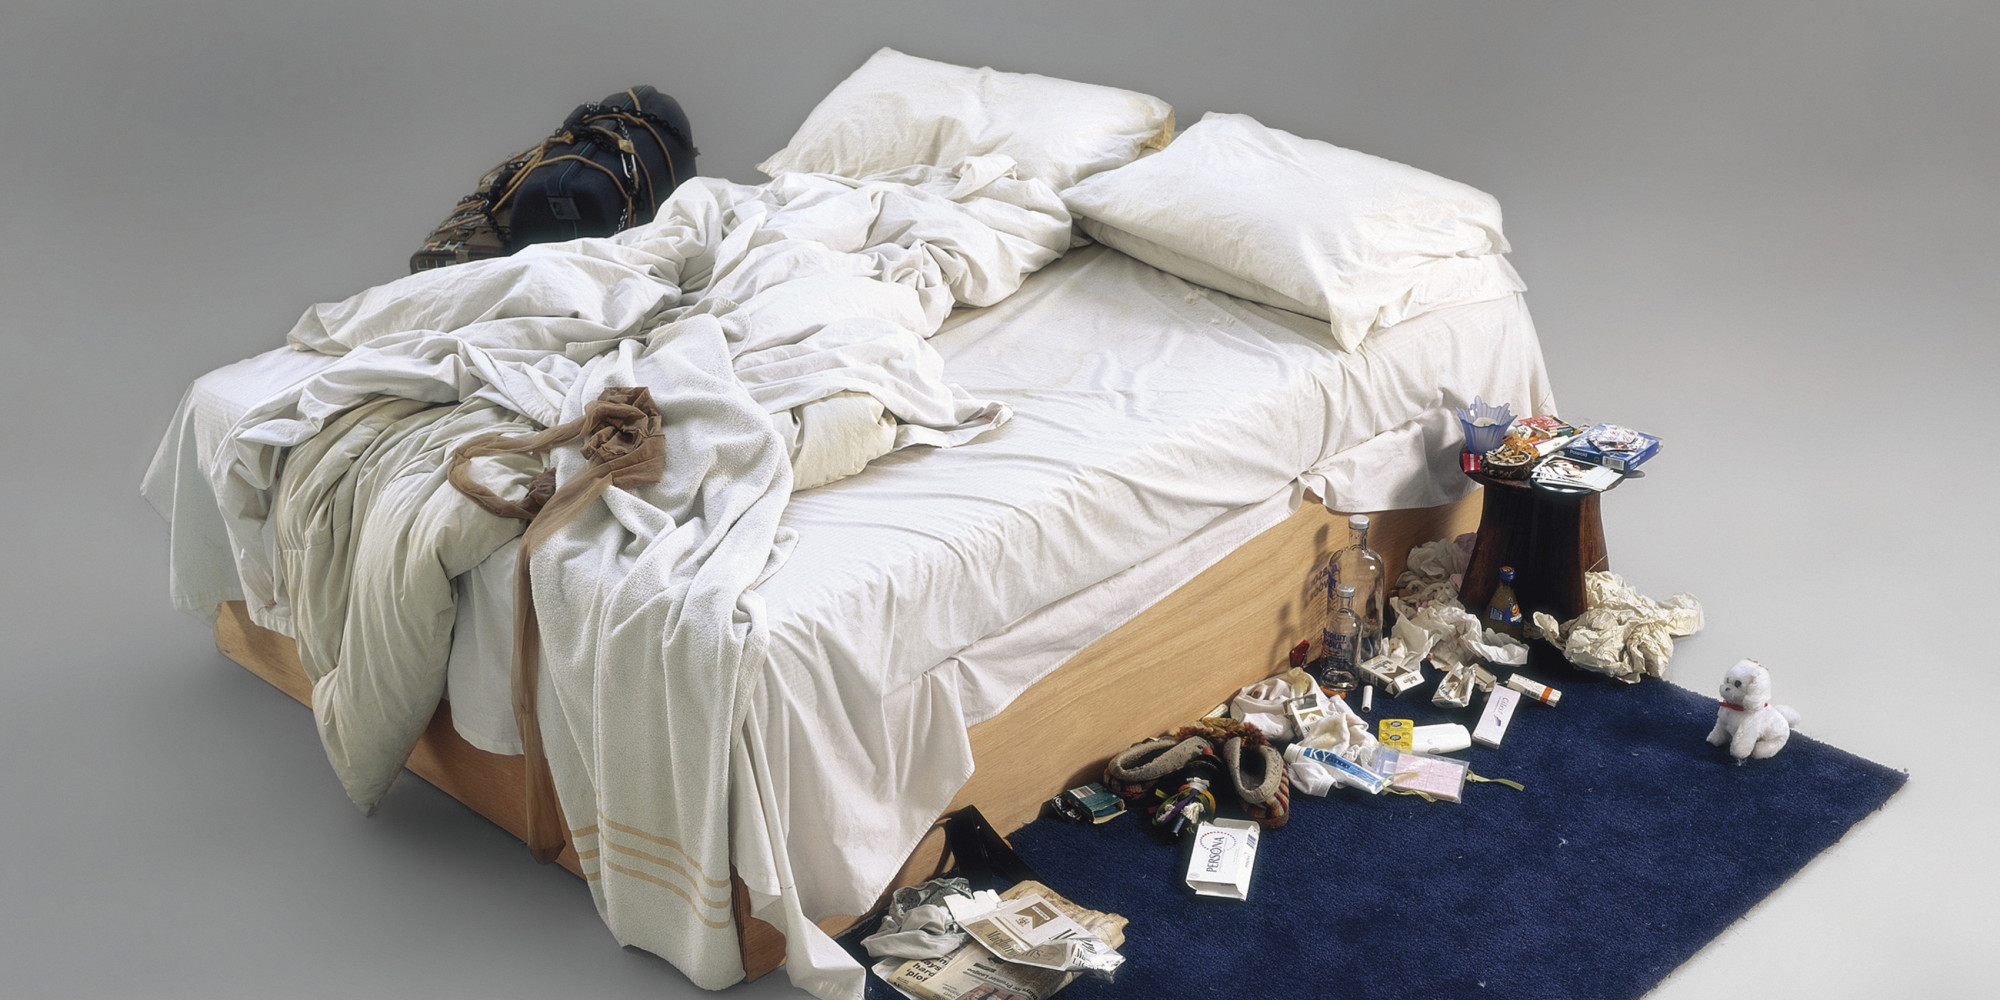
\includegraphics[height=6cm]{graphics/tracey-emin-my-bed.jpg}
  \caption{Tracey Emin, \textit{My Bed}, 1998}
  \label{fig:TraceyEmin_MyBed}
\end{figure}

Tracey Emin puts her private life to the public via representation of her bed. This work can be as a portrait of artist in a post-modern fashion. Around the bed, there are pieces of junks speared all over the room. It can be understood from her junk what type of life she has. To put it another way, viewer enter the world of the artist through her trashes.

Every detail of Emin’s private life is presented through her bed in an uncensored fashion. The idea of \textit{My Bed} (Figure \ref{fig:TraceyEmin_MyBed}) was result of a depressive period in the artist’s life when she had stayed in bed for a few days without eating or drinking anything except alcohol. The feeling of depression resulting in mess and detritus is not completely unusual to many people, and \textit{My Bed} therefore has a bold affect on the viewer. The artwork generated great media enthusiasm, particularly over the fact that the bed sheets were stained with bodily secretions and the floor had items from the artist’s room, such as condoms, underwear with menstrual blood stains, other junks, and functional, everyday objects, including a pair of slippers. 

It is a realization what she did during her depression time and perfectly represents her condition during those days. It can be understood that trash is part of our life. Things that are exhibited in this work are part of her action. She created them and later through them in the mind of people the condition and life of Tracey Emin are recreated.

The work can be interpreted as a self-portrait of a woman at a time of emotional depression. However, it is still a bed and all that a bed symbolizes and covers life events such as sleep, sleeplessness, sex, birth, death and dreams. Further bedroom is one of the most personal spaces in the homes. Particularly for the ones that have small rooms and spaces bed becomes a life space. I have also experienced such a thing at boarding school and university dormitory for total my eight years. Having tight space sometimes bed becomes a place for studying and reading. Sometimes it was used to dry the clothes. It is more than sleeping and provide place for other activities.



%****************************************
\section{Žižek’s Approach to Rubbish}
Last decades there is an increasing attention the ecology and rubbish. Global warming is one of them, plastic pollution on the oceans also is part of it. These types of news and talks increasingly find a place on media more and more. At this stage, Žižek comments on ecology and trash conversely.

\begin{quote}
In the late twentieth century, in the context of increasing environmental awareness, this consciousness has altered yet again, and waste has been revalued and recoded from rubbish to recyclable resource, it has moved from the bin to the compost heap, it has insinuated itself into our lives in different ways and with different effects \citep[5]{hawkins2005ethics}.
\end{quote}

In the documentary film Examined-life Žižek dressed as a sanitation man discusses ecology in the middle of a dump in London. His part starts with these sentence: \quotes{This [dump] is where we should start feeling at home}. The place where he talks is a site for depositing people’s excess and unwanted material. It is a place of out of sight.

He draws attention that the thrown out garbage only disappears from people’s living environment. Particularly discarding it is an action of escape from the unwanted. However, it still exists in reality and waits at somewhere else. Strictly speaking, it does not disappear, moves away.

According to Žižek, the way of approaching ecology is problematic in current societies because of accepting nature as a balanced, and harmonious. He claims that it is ideological in the sense that \quotes{wrong way of thinking and perceiving reality.} The meaning of ideology is here mystification of real problems. He claims that one of the key mechanism of ideology is temptation of meaning. In other words, people search for meaning when a terrible event happens in order to make it easier to accept. He opposed the notion of the existing world is in the best possible state and that humans disturb nature. According to him, nature is not an balanced organism that humans exploit, but rather a series of \quotes{unimaginable catastrophes} by asking the question what type of disasters would happened on the earth to compose oil that is a significant source of energy. Žižek asserts that ecology will slowly turn to a conservative ideology that is a kind of an unquestionable highest authority. Its voice is like \quotes{Do not mess with D.N.A. Do not mess with nature.} In the light of these arguments instead of talking from an authoritarian high ground, he suggests that to find poetry and spirituality in the dimension of rubbish people create. He thinks that that is the true love of the world by asserting that \quotes{love is not idealization.} Therefore, that is the reason why he thinks that a dump is a place that people should accept it as a home. 

In the light of Žižek’s arguments ecology is not an appropriate (or enough) point to approach trash. He points out the need for new approaches to trash. This new approach should not idealize nature and trash. At this point, the practices of art gain importance to establish new understanding of trash. Not every act of transforming trash is not related to ecological concerns. Artists are not trying to save the planet earth. Beyond ecological concerns, they are attempting to find new ways to look and live with trash. Some artists turned to trash into site-specific sculptures that are more than trash heap after their intervention. Not discarding but embracing people's trash, they turned them to a something that worth it to watch and think about it. They convert what people throw away into objects that are harmonious with the existing system because it is not possible to think that nature will live harmoniously with what people created. The more reasonable idea will be people will live harmoniously with what they create. Their action can be seen as turning trash to things that can be lived together.

In the light of this arguments the idealization of nature is problematic. Loving nature is loving it with all dimensions. His suggestion is to find a way to live with trash instead of seeing it as trash. Then the question becomes how to love and live with trash? Think beyond the common perception. Do not consider it as abject, disgust. Can live with our trash enrich our perceptions and abilities? How not to see them as trash and useless? Can it be possible with art?



%****************************************
\section{Rubbish Theory}
Objects have a lifetime similar to humans, and they do not remain same through that time. They move around, and their value, usage, location change constantly. During their lifetime objects may circulate different markets and values systems such as economic, social and aesthetic. Especially these cycles have accelerated with the arrival of consumer culture. For instance, most recent technological devices become outdated within a few years. Firsthand, secondhand and even trash is exchanged among not only people but also countries. People from other cultures and understanding interpret objects differently. They often are not aware of their initial and intended usage. They find new original purposes and meanings. Therefore, objects turn different items in their hand. Anthropologist Sidney Mintz \citep[as cited in][]{strasser1999waste} writes that \quotes{I have seen automobile bearings fashioned into portable vulcanizing kits; bits of toothbrush handles used as \singlequotes{jewels} for rings, and ordinary tin cans turned into simple kerosene lamps.} As it can be understood that objects function and value are transformed by relocation and revaluation of objects from one place to the other or one discipline to another. 

It can be claimed that the end of an object’s life corresponds to the moment when it is refused. As stated by \citet[63]{emgin2012trashion} this action \quotes{might take place in different forms and for [various] reasons.} In common sense, trash can or dump is the graveyard of objects. In landfills, \quotes{the object is left valueless} in all kinds various value system. \quotes{It can no more serve a function, it can on no account be exchanged for anything else, and it can by no means engage in the processes of signification to connote and endow its user with specific social values} \citep[63]{emgin2012trashion}. However, Thompson’s \textit{Rubbish Theory} shows us the opposite of it. Trash can is not an end it is starting point of another life.

In \textit{The Social Life of Things} \citet[3]{appadurai1986social} highlights that \quotes{commodities, like persons, have social lives.} Similarly, \citet[66]{kopytoff1986cultural} notes that the biography of a thing was significantly similar to an account of someone’s life. It moves into different positions, and experiences diverse paths in the course of different states and different systems of value that are both economically and culturally defined. Appadurai focuses on the \quotes{commodity potential} of things and asserts that \quotes{things can move in and out of the commodity state, that such movements can be slow or fast, reversible or terminal, normative or deviant} (1986: 13). However, one can ask that what are these commodity states and does anything exist between them? Thompson’s \textit{Rubbish Theory} fills this gap.

Thompson observes the creation and destruction of value in products, cultural artifacts, and ideas. He notes that how an item’s economic and cultural value lessen through time rendering the objects unprofitable or unnecessary and how others’ value increases. In his notable \textit{Rubbish Theory}, he declares three object states; transient (normal state, decreasing value, circulating), durable (permanent, increasing value, removed from circulation) and rubbish (zero value, will be destroyed or reinvested for economic and social value). The transient category falls into the common state of objects that are lessening in value and have limited life period. A used car can be an example of transient state. On the contrary, the durable objects’ value increase through time and have probably unlimited life spans. Antiques and objects in museums can be an example of durable. This theory gives rubbish a key role between transient and durable.

Rubbish is, by definition, an object state that is not or is no longer, owned by anyone, which falls outside all kinds of economics, culture, and social system. As one of many things on the garbage heap, a discarded object even tends to take on a negative value as something unsanitary, dangerous. However the socially constructed value of the object can shift through time from its limited life span of usefulness and meaning to a infinite and valuable socially accepted rubbish.

The potential of the discarded material also relies on its status as an object approaching a zero point of value. In other words, it has reached a point in transition between the world of the functioning, the useful and visible, and the realm of the invisible, the non-functioning and empty. Its value and function open to be reset. As Thompson suggests that rubbish is both ripe for disappearance and yet suitable for reinterpretation, reinvestment or revaluing. Further rubbish as a state of being flexible is ready to transformation.

Similar to Žižek’s claim, that is \quotes{trash does not disappear}, Thompson notes that \quotes{in reality ... [trash] just continues to exist in a timeless and valueless limbo, where, at some later date (if it has not by that time turned, or been made, into dust) it has the chance of being discovered.}

As argued by Thompson, rubbish represents a remarkable in-between ---middle--- category in a area of flexibility which is not exposed to the same control systems of the valuable and socially considerable categories of transient and durable. Hence, it \quotes{is able to provide the path for the seemingly impossible transfer of an object from transience to durability} (1979: 9) he also puts forward that \quotes{a transient object gradually declining in value and in expected life span may slide across into rubbish} (1979: 9) where it has the chance of being re-discovered, brought to light or admired once again. In other words, he specifies the path between the object categories. The path of transitions between transient, rubbish and durable objects are defined as follows: from transient to rubbish (transient -> rubbish) and from rubbish to durable (rubbish -> durable).

To illustrate \textit{Rubbish Theory} the series of compression by French sculpture César can be analyzed in the context of it. His early work is composed of soldered and welded metal as well as junk materials. In 1960, Caesar discovered the hydraulic press that is capable of compacting scrap metal (especially car bodies) during on a visit to a scrap merchant in search of metal. He admired from the hydraulic crushing machine in operation and started to experiment with it in his sculptures. The machine is used to compress the metal items in order to gain from space. His first three automobile compression exhibited at Salon de Mai in 1960 and bring him a supportive fame. Later Viscountess Marie-Laure de Noailles who is important figure of these ages, gave him her Zim model car to compress. It is 
% http://www.sothebys.com/en/auctions/ecatalogue/2015/art-contemporain-pf1515/lot.6.html
\quotes{a revolutionary artistic gesture then, but also a strong political gesture, right in the middle of the Cold War; César having chosen to lash out against a Zim, a jewel of the Soviet automobile industry commissioned by Khrushchev at the beginning of the 1950s to compete with the Cadillac.} Additionally car was one of the most desired possessions of people in twentieth century. Through the eyes of rubbish theory it is a transient object and after the intervention of artist, it is transformed into an artwork that preserved in the collection of Museum. In other words, it switched to durable category by interestingly trashing it.

\begin{figure}[h!]
  \centering
  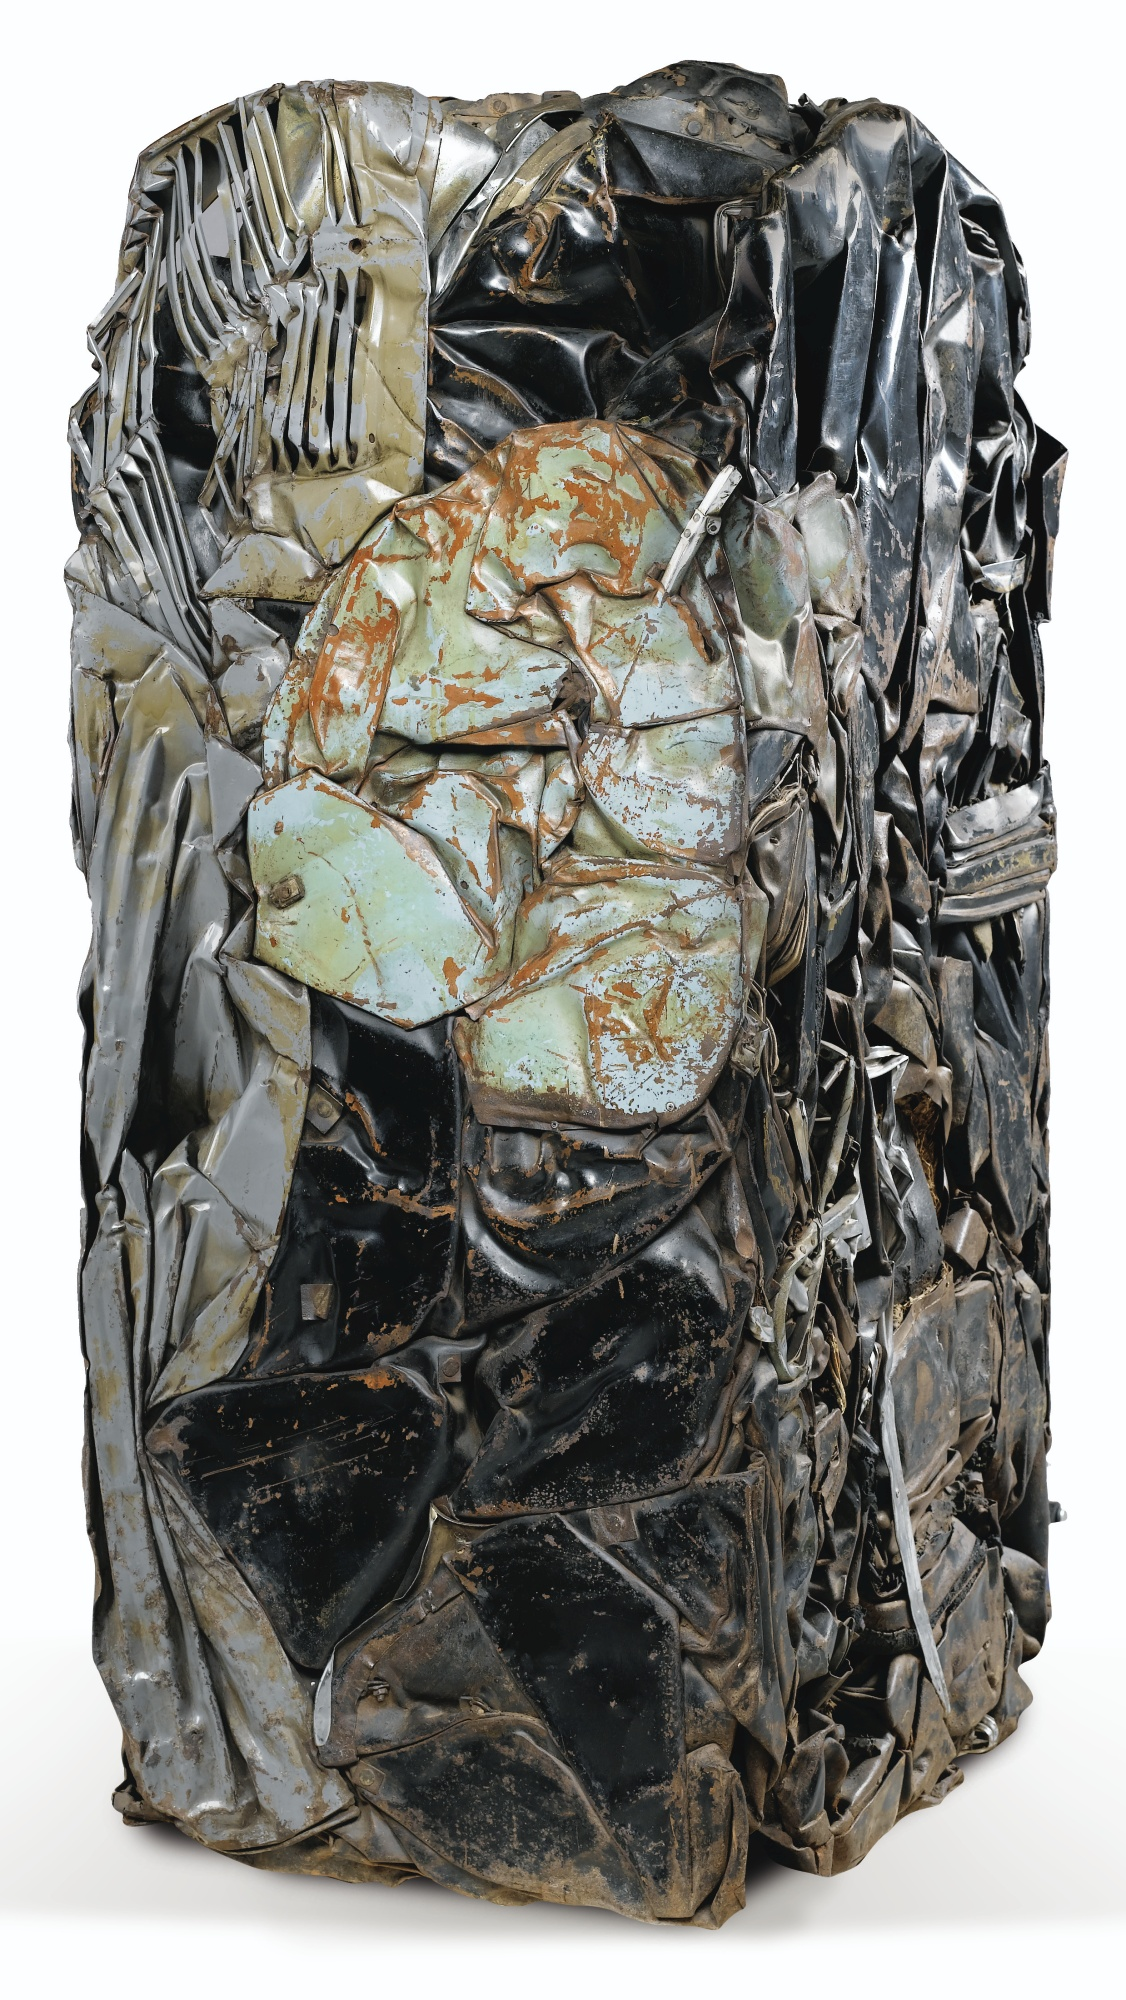
\includegraphics[height=10cm]{graphics/Cesar_Zim.jpg}
  \caption{César Baldaccini, \textit{Compression Zim}, 1960-1961, 157 x 82 x 64 cm}
  \label{fig:Cesar_Zim}
\end{figure}

Although Thompson is quite successful describing states of objects, claimed transitions between object categories in the theory have some problems. Thompson label some transitions as possible and the others as impossible. He only allows movement of goods from transient to rubbish, and from rubbish to durable. Movement in the other directions, from durable to either transient or rubbish, does not allowed in this system. However, Duchamp’s notable ready-made \textit{Fountain} is one of the examples that fall outside of the given transitions.

\textit{Fountain} (1917) is an artwork produced by Marcel Duchamp, who is notable member of provocative Dada movement. The piece was an industrial porcelain urinal, which was signed \quotes{R.Mutt}. It is submitted for the exhibition of the Society of Independent Artists in 1917. Committee rejected \textit{Fountain}, even though the rules declared that all artworks would be accepted from artists who paid the fee. It is considered one of the major artworks of the twentieth century because of challenging the existing understanding of art. Duchamp used already existing fabricated ordinary urinal to express his ideas by challenging existing way of art making which requires efforts of the artist. It forces to the limits of the language of art and perception the art. To understand his works requires shift inside of the peoples mind. For him, the idea is important rather than the object. He also criticized the position of artist by signing urinal as \quotes{R.Mutt} who is actually not exist. In the editorial The Blind Man summarized this work as follows: \quotes{Whether Mr. Mutt with his own hands made the fountain or not has no importance. He CHOSE it. He took an ordinary article of life, placed it so that its useful significance disappeared under the new title and point of view --- created a new thought for that object} \citep{duchamp1917mutt}. To debate all the aspects of this work is not possible with the scope of this thesis. However when it is analyzed through the frame of rubbish theory, urinal a transient object turned to durable objects that are exhibited by the intervention of artist. Urine titled as \textit{Fountain} is still functional and have a place in the market. In another word, it is not rubbish.

\begin{figure}[h!]
  \centering
  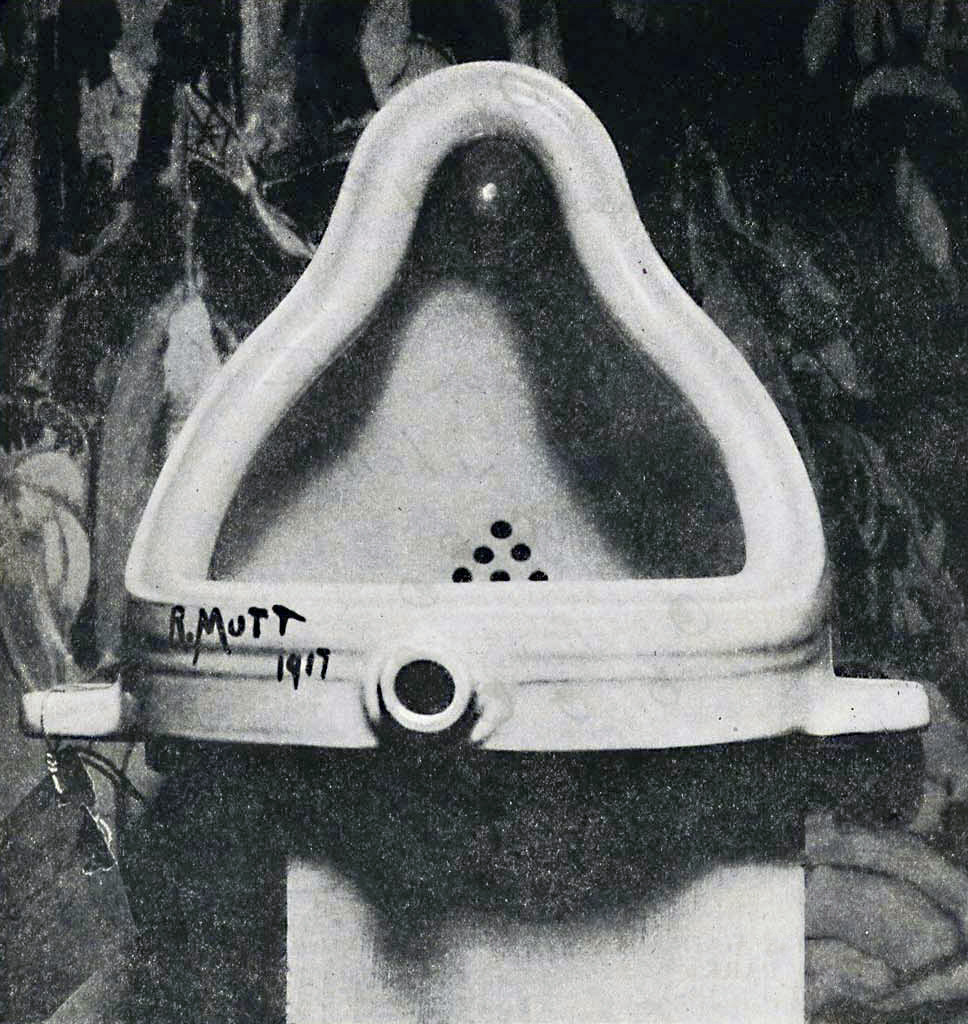
\includegraphics[height=6cm]{graphics/Duchamp_Fountaine.jpg}
  \caption{Marcel Duchamp, \textit{Fountain}, 1917, Porcelain urinal}
  \label{fig:Duchamp_Fountaine}
\end{figure}



%****************************************
%\subsection{Rubbish Theory in Practice: From Rubbish to Durable}
%\paraphrase{In rubbish theory beyond the objects states how it happens transition of objects in practice is missing and Parsons fills this gap by claiming that transition from rubbish to durable are possible with finding objects, displaying objects, re-using objects \cite{parsons2008thompsons}.} (finding paper, transforming to notebooks and giving away them to create an opportunity to be displayed different location and times.) 

%Three such sets of practices are explored below, they include: finding objects, displaying objects and transforming and re-using objects. It is argued that each of these sets of practices changes the way we view an object moving it from being seen as a ‘rubbish object’ of no value to a ‘durable object’ of increasing value.

%\textbf{Finding Objects:} One key way in which objects may slide from the category of rubbish to durable is through the act of finding. Indeed, Gabriel and Lang (1995) include the ‘Consumer as Explorer’ as one of many possible consumer identities. What, then might one mean by ‘the find’? Ultimately the find relates to discovery, and suggests that something has been otherwise overlooked, ignored or hidden away. The find may not involve objects which are new to us, it is possible to find some of ones own items if they have been hidden away long enough in an attic and thus made strange to us. The concept of the find also suggests that the found object has some qualities that others (or indeed ourselves) have in the past overlooked, as such it is closely related to ‘bringing to light’. The find may be extended to embrace features of objects as well as objects themselves. This directs us to their ‘potentialities’, objects may have been there all along but we’ve suddenly found them to be useful, likeable or beautiful. It might be that some aspect of them has simply been brought to our attention. Equally, as discussed below in relation to transforming objects, we may make alterations to objects which bring out their potential. The transition from thing of little or no value (rubbish), to thing of value (durable) can result form a relatively minor shift in the way we see something.
%........................................



%****************************************
% Theoretical Analysis of Found Object
% (Summary From Paul M Camic.)
%\summary{Theoretical Analysis of Found Object}
%\paraphrase{As a species Homo sapiens has been gathering and collecting objects for thousands of years. Food, clothing, weapons, fuel, animals, and plants are the more obvious items, but visually pleasing objects, things that arouse curiosity, and shapes that stimulate the imagination have also been sought. The search for “things,” collecting them (Humphrey, 1979), and the need to embellish and make the ordinary special (Dissanayake, 1988) have been essential parts of the evolutionary process of human development (Bettinger, 1991; Dissanayake, 1992). For example, many early cave drawings occur around a natural feature within the cave such as a projection or indentation (Bahn, 1998; Lewis-Williams, 2004), making these natural features potentially comparable to found objects in modern and contemporary art (Read, 1930). When early prehistoric eople recognized a cave’s natural feature as a “found object” and incorporated it in a picture, it is possible that the natural feature took on a higher value than if left alone, thus adding to the value of the object on the cave wall. Once found and incorporated in paintings and drawings on a cave wall, it is possible that these protrusions and indentations became objects that functioned symbolically.}

%\paraphrase{In contemporary societies, people seek objects to adorn bodies, decorate homes and gardens, and personalize places of work (Menzel, 1994). Seeking and finding objects, whether in vast Asian cities, remote African villages, or the high streets of Europe and North America, have become part of daily life for millions of people. Although most of these objects are purchased new in shops or online, many others are preused items, castoffs, or trash found in back alleys and country lanes, dumpsters, and rubbish bins or purchased cheaply in flea markets, garage and boot sales, and in shops catering in previously owned goods. Some individuals have chosen to salvage objects out of economic necessity, as depicted in Jean-Francois Millet’s 1857 painting The Gleaners and by Agne`s Verga’s 2002 documentary film Les Glaneurs et la glaneuse, whereas others have done it for a range of other reasons, including a desire to rescue them (Belk, Wallendorf, \& Sherry, 1989). These “other reasons” pose an opportunity for researchers to better understand why people voluntarily seek society’s discarded material objects and how they make use of them. A form of cultural reuse, the process of salvaging and using found and second-hand objects has potential implications for \ldots}
%........................................





%\textbf{Displaying Objects:} by displaying objects in home, fashion etc. (This is not a strong category.) Maybe publicly exhibiting them. 

%\textbf{Transforming and Re-using Objects:} These transformations may involve creating new uses for old things to fit in with contemporary lifestyles. Transformations may also involve the modification or updating of objects through painting, alteration or repair. Transformations may not only be based around creating new uses but also creating new looks. The re-use of objects also creates value for things that otherwise would be allowed to slip away (or slide terminally into the rubbish category).




%Moving nature of trash/objects. Objects value/state is not static open to intervention, has potential to be reconsidered. Their place shift in the society. Classification is the main key, being trash is not related with the object property. It is about perception the trash.

%First part analysis trash of disposable items and the works of art that looks differently to these trash. Whose trash? Which trash? Answers these questions. It displays common approach to the trash. Artist reflection to them. When we look at personal level (previous one is general one) discards tells us about our activities, possessions, preferences etc. They can be viewed as portrait of artist and us.

%Firstly trash is created (by the throwaway culture). Even if there is counter argument about it, the focus is disposable items and their amount is very high. After generating mountains of garbage the approach of Žižek introduced. What to do this garbage see. He claims that we need to find a way to handle it. Find aesthetics and other things. Learn to live with the trash.

%Later rubbish theory and relative approach to the trash. Trash is not static. Objects are not static. It related with the perception.

%Thompson thinks that the switch only occurs when all the value to the given object is removed. To gain a new value, meaning and purpose it must be exit from previous system.  Changing the context can only be possible first rubbishing them or loosing all value.

%Thompson and Zubiaurre say trash moves among various range of value systems. 

%Žižek says you must find a way of loving your trash, or a way of living with trash instead of idealization of nature and waste. Purification is not suggested by him.

\chapter{TRASH (IN) ART}



\begin{singlespace}
\epigraph{One day, in a rubbish heap, I found an old bicycle seat lying beside a rusted handlebar, and my mind instantly linked them together. I assembled these two objects, which everyone then recognized as a bull’s head. The metamorphosis was accomplished, and I wish another metamorphosis would occur in the reverse sense. If my bull’s head were thrown in a junk heap, perhaps one day some boy would say, \quotes{Here’s something that would make a good handlebar for my bicycle!}}{\hfill ---Pablo Picasso, \textit{Trashformations}, 1998}
\end{singlespace}



This chapter questions the purpose and meaning of using trash as a medium in the artworks. Reasons and motivations of artists who use trash will be elaborated. Artists who use discarded items in their work will be analyzed in the light of arguments discussed in the previous chapter. Here, the main question is why artists select to use society’s debris rather than fresh items. Hence, my research will focus on the place of trash in the world of art by looking at different methods and approaches. The scope of this research is started from masterpieces and founding works, and continued with recent examples of artworks.

Firstly I look at how artist started using objects that are not produced by herself/himself and with the purpose of making art. Considered early works are notable and founding ones that open new dimensions to reconsider objects and their meaning. Further, they extended the ways of art making and the language of art. Therefore, it is important and necessary to analyze them. In other words, I first look at the foundation of using non-art objects in the art making. Early examples are analyzed and how they evolved over time is explored. I try to find out how they affected successor artist. Secondly this chapter looks some examples of contemporary works. Particularly, I try to capture the current approaches on trash. Several methods and genres are explored. Lastly focused on the inspiring documentary of Agnès Varda, The Gleaners and I, which provides a general picture of the subject.



%****************************************
\section{Root in the Art History}
Using trashed objects in making art can be examined with the use of non-art objects in modern art. In other words, some artist started using objects in different scope beyond their intended purpose or intended meaning and function in their modern artworks. They develop their artworks by using paper and other stuff by pasting or juxtaposing them together.

From the beginning of twentieth century-century non-art objects draw attention of artists. Usage of these objects play significant role in the development of art trough time. Usage of these objects dramatically changed the way how people look at art. In short, they introduced a new way of making art.

One of the remarkable change in twentieth century-century art is the use of unconventional materials in the making of paintings and sculptures, rather than the conventional materials produced with the purpose of art. These objects are not commonly recognized as art often because they already have a non-art function. Their place in the society and people’s mind commonly have a different meaning. Beyond that, artists started to use them for their own purposes. Thus, objects gained different meanings and usages with the hands of artists. It is explained in the previous chapter that objects are not static and absolute. Objects can be used for new purposes even if they lost their meaning and value in the conventional system.

Modern artist questioned the way of traditional way of art making in every dimension. Their approach is out of the previous methods. They are looking for the beyond of painting. With using different objects they break the pureness of artwork. It is not pure anymore, it is fragmented. They push the boundaries of art. Using non-art objects in the production of art challenges existing conventions of painting.

Using non-art object can be considered as moving away from the purification of art which is also significant movement in modern art. Purification argues the separation of art and the others. Abstract and minimalist works can be given as an example to the purification. However, methods such as collage and assemblage are a composition of different fragments and pieces. Rather than the traditional way of painting on canvas modern artists composed their work with the combination of various objects from different context. With this approach works can be examined in multi-dimensional context. This also represents another branch in modern art.

In twentieth century-century, modern artists experimented with new ways of seeing and with fresh ideas about the nature of materials and functions of art. Previously paintings are based on linear perspective and realistic style. Themes are often composed of religious and mythical narratives. After the second half of the 19th-century, they started to abandon these themes and painting methods. For instance, in the works of impressionist paint brushstrokes can be easily identified. In impressionist paintings, themes are composed of everyday scenes. With Cezanne, the linear perspective is started to question and later this questioning reached to its peak point with cubism. Cubism is developed with the collaboration of Picasso and Braque. Besides, these two artists experimented non-traditional materials in their works for the first time in the scope of fine art. They continuously produced works with using different objects. They support each others art. They showed that an endless potential lay there. They collaborated with each other on the development of cubism and collage. One of the keys to understand the significance of Cubism of Picasso and Braque, is to view their actions and how unusual they were for the time. When they placed mass produced artifacts into the realm of fine art they acted as artistic iconoclasts of their age.

Collage originates from the French \textit{coller} is a technique of pasting together manufactured, printed, or found materials, such as pieces of newspaper, fabric, wallpaper to a panel or canvas, frequently in combination with painting. In about 1912–13 Pablo Picasso and Georges Braque extended this technique, combining fragments of paper, oil-cloth, and newspapers with oil paint on canvas to construct compositions. Pasting paper is not a new technique but using this technique it in the art making is a revolutionary movement in the language of art \citep{waldman1992collage}. \quotes{Collage was a major turning point in the evolution of Cubism\footnote{It needs to be noted that there is two types of Cubism; analytical and synthetic. Analytical one early phase of cubism and based on fragmentary appearance of multiple viewpoints and overlapping planes. On the other hand synthetic one is the successor phase of analytical one and formed with various textures and patterns.}, and therefore a major turning point in the whole evolution of modernist art in this century} \citep{greenberg1984collage}.

Similar to the collage, assemblage is produced by the incorporation of three-dimensional objects. \cite{seitz1961art}, the curator of the exhibition \quotes{The Art of Assemblage} featured at the New York Museum of Modern Art in 1961, described assemblages as being made up of preformed natural or fabricated materials, objects, or fragments not designed as art materials.

One of the earliest and notable examples of collage is Picasso’s \textit{Still Life with Chair Caning} (Figure \ref{fig:Picasso_Chair}), in which a piece of oilcloth which is used as tablecloth or self coverings with an imitation chair caning design was pasted onto the painting. This work of Picasso also can be considered as first example of assemblage because of a rope that was used to frame the picture. Picasso combined painting with already existing materials. As mentioned in the name of the work, Picasso give clues of the parts of it. For instance the oval canvas and the rope around it represent the table. Pasted chair caning signifies the chair near the table. On the table folded paper shadow represent newspaper. Further there is a cut out lemon painted onto the table. The three letters above the scrap of cloth, \quotes{JOU}, can be understood as both the beginning of the word \quotes{JOURNAL}, referring to the customary newspaper lying across the cafe table, and as the French verb meaning \quotes{to play.} The new technique of collage provided new possibilities of playfulness. This was a new way of making art; instead of painting an object or landscape, you could paste whatever it was right onto the canvas.

\begin{figure}[h!]
  \centering
  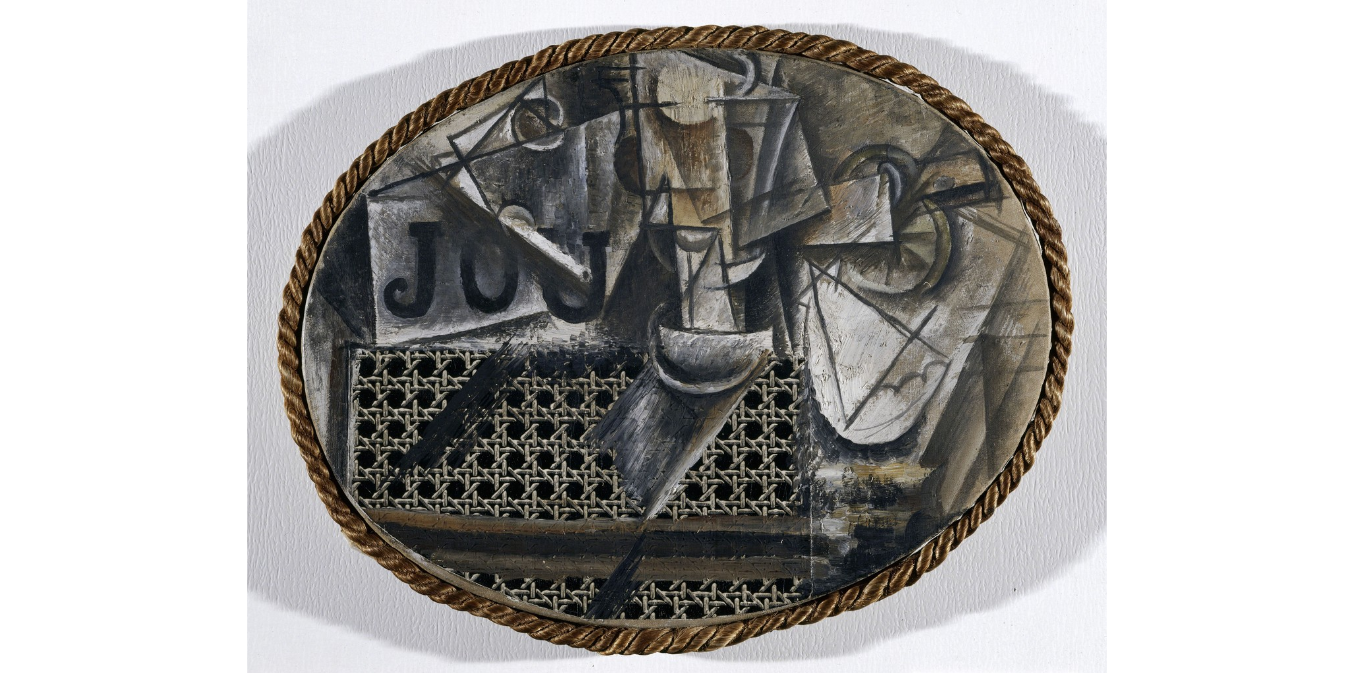
\includegraphics[height=6cm]{graphics/picasso_chair.png}
  \caption{Pablo Picasso, \textit{Still Life with Chair Caning}, 1912, oil on oil-cloth over canvas edged with rope, 29 x 37 cm (Musée Picasso)}
  \label{fig:Picasso_Chair}
\end{figure}

Moreover, Braque and Picasso questioned the elitism of the art world, which had always dictated the separation of common, everyday experience from the contemplative realm of artistic creation. Of equal importance, their work highlighted and separated the role of technical skill from art-making. Braque and Picasso introduced a fake element on purpose, not to mislead or fool their audience, but rather to force a discussion of art and craft, of unique and mass-produced objects. They inquiry as \quotes{Can this object still be art if I don’t actually render its forms myself, if the quality of the art is no longer directly tied to my technical skills or level of craftsmanship?}

After Picasso and Baraque, many artists applied collage and assemblage techniques to their works. Dada artist Kurt Schwitters is one of the productive artists among them. In 1918 he created his own form of Dada in Germany named \textit{Merz}, using rubbish elements such as newspapers, bus tickets and pieces of broken wood in his collages and constructions. The nonsense word \textit{Merz} is generated from the name of a bank: the Kommerz und Privatbank. \textit{Merz} was soon to become a kind of brand name for almost all his productions. \cite{webster2011kurt} puts significance of Schwitters in the development of art as follows:

\begin{quote}
The language of \textit{Merz} now finds common acceptance and today there is scarcely an artist working with materials other than paint who does not refer to Schwitters in some way. In his bold and wide-ranging experiments he can be seen as the grandfather of Pop Art, Happenings, Concept Art, Fluxus, multimedia art and post-modernism...

Schwitters’ work inspired such post-war pioneers as Jasper Johns, Robert Rauschenberg and Joseph Beuys, and he is now seen as the grandfather of post-1945 art movements, from Pop Art to Fluxus, Conceptual Art to site-specific art, and the forerunner of present day artists such as Thomas Hirschhorn, Gregor Schneider and Rachel Whiteread.
\end{quote}

He is very insisted on what he did. He constructed his room sized construction \textit{Merzbau} several times in different locations. First one destroyed in the Second World War, the second by fire in 1951 and the only third one was preserved. They are never ending structures not static. Through his life he added bits and pieces to them. \cite{carroll2011ruin} explains art of Schwitters as follows:

\begin{quote}
The German avant-garde was working from ruins literally and metaphorically, and trash was both practically and freely available; to use it was an action that took the ruins of our society, its discarded, to question how meaning is constructed. Schwitters is able to use the ruined, the waste products, as an anthropological exploration of society from both its unpleasant outcomes and its decay. \ldots trash was both practically and freely available; to use it was an action that took the ruins of our society, its discarded, to question how meaning is constructed. As he wrote: \singlequotes{It grows more or less according to the principle of a metropolis.} The \textit{Merzbau} was itself a city; and just as Marx wrote that it was not the materiality of the object but the social relations that create value, the use of urban detritus in particular, the squalid results of mass-produced human relations, infuses the materiality of Schwitters’ work with an anthropological quality. Material has transformed into information, and \singlequotes{how} has surpassed \singlequotes{what} we see. The grottos in the \textit{Merzbau} that still reveal this detritus most clearly could not be re-created in Bissegger’s reconstruction because, arguably, they are an exploration of absence, an exploration of ruin.
\end{quote}

Jacknis \citep[as cited in][]{cerny1996recycled} claims that \quotes{like collage in art or quotation in literature, the recycled object carries a kind of \singlequotes{memory} of its prior existence. Recycling always implies a stance toward time ---between the past and the present--- and often a perspective on cultures ---one’s own and others.}

Reused objects contain within them a reference to many separate times. Whatever their final design or destination, these reused non-art artifacts are, by definition, impure, inauthentic products of past and present, here and there, us and them \citep{cerny1996recycled}.

It is claimed that the end result is a category of hybrid objects that bear the mark of at least two distinct domains, each with its won material, meaning, makers, and users \citep{cerny1996recycled} Whatever their final function, each of these objects contains within itself a visual, material, and conceptual reference to multiple technologies, histories and places.

Collages and assemblages can be composed of all types of objects such as trash and found object. The notion of found object is researched by many scholars \cite{camic2010trashed, gascoyne1935short}, but usage in the art has gained new dimensions with the Duchamp’s concept of ready-made. Industrially manufactured or anything found  anymore can found a place in the art. The most notable example is \textit{Fountain} (discussed in the previous chapter), a standard urinal purchased from a hardware store and displayed on a pedestal, resting on its side. Before that first one is \textit{Bicycle Wheel} (Figure \ref{fig:Duchamp_BicycleWheel}). He wrote that the idea of a bicycle wheel upside down onto a stool. Although he claimed to select objects for his ready-made without regard to beauty, he said, \quotes{To see that wheel turning was very soothing, very comforting\ldots I enjoyed looking at it, just as I enjoy looking at the flames dancing in a fireplace.} These samples were the beginning of 
shift from an art that is striving for beauty to a higher complex or hidden meaning beyond what was seen from common artifacts found in everyday living.

\begin{figure}[h!]
  \centering
  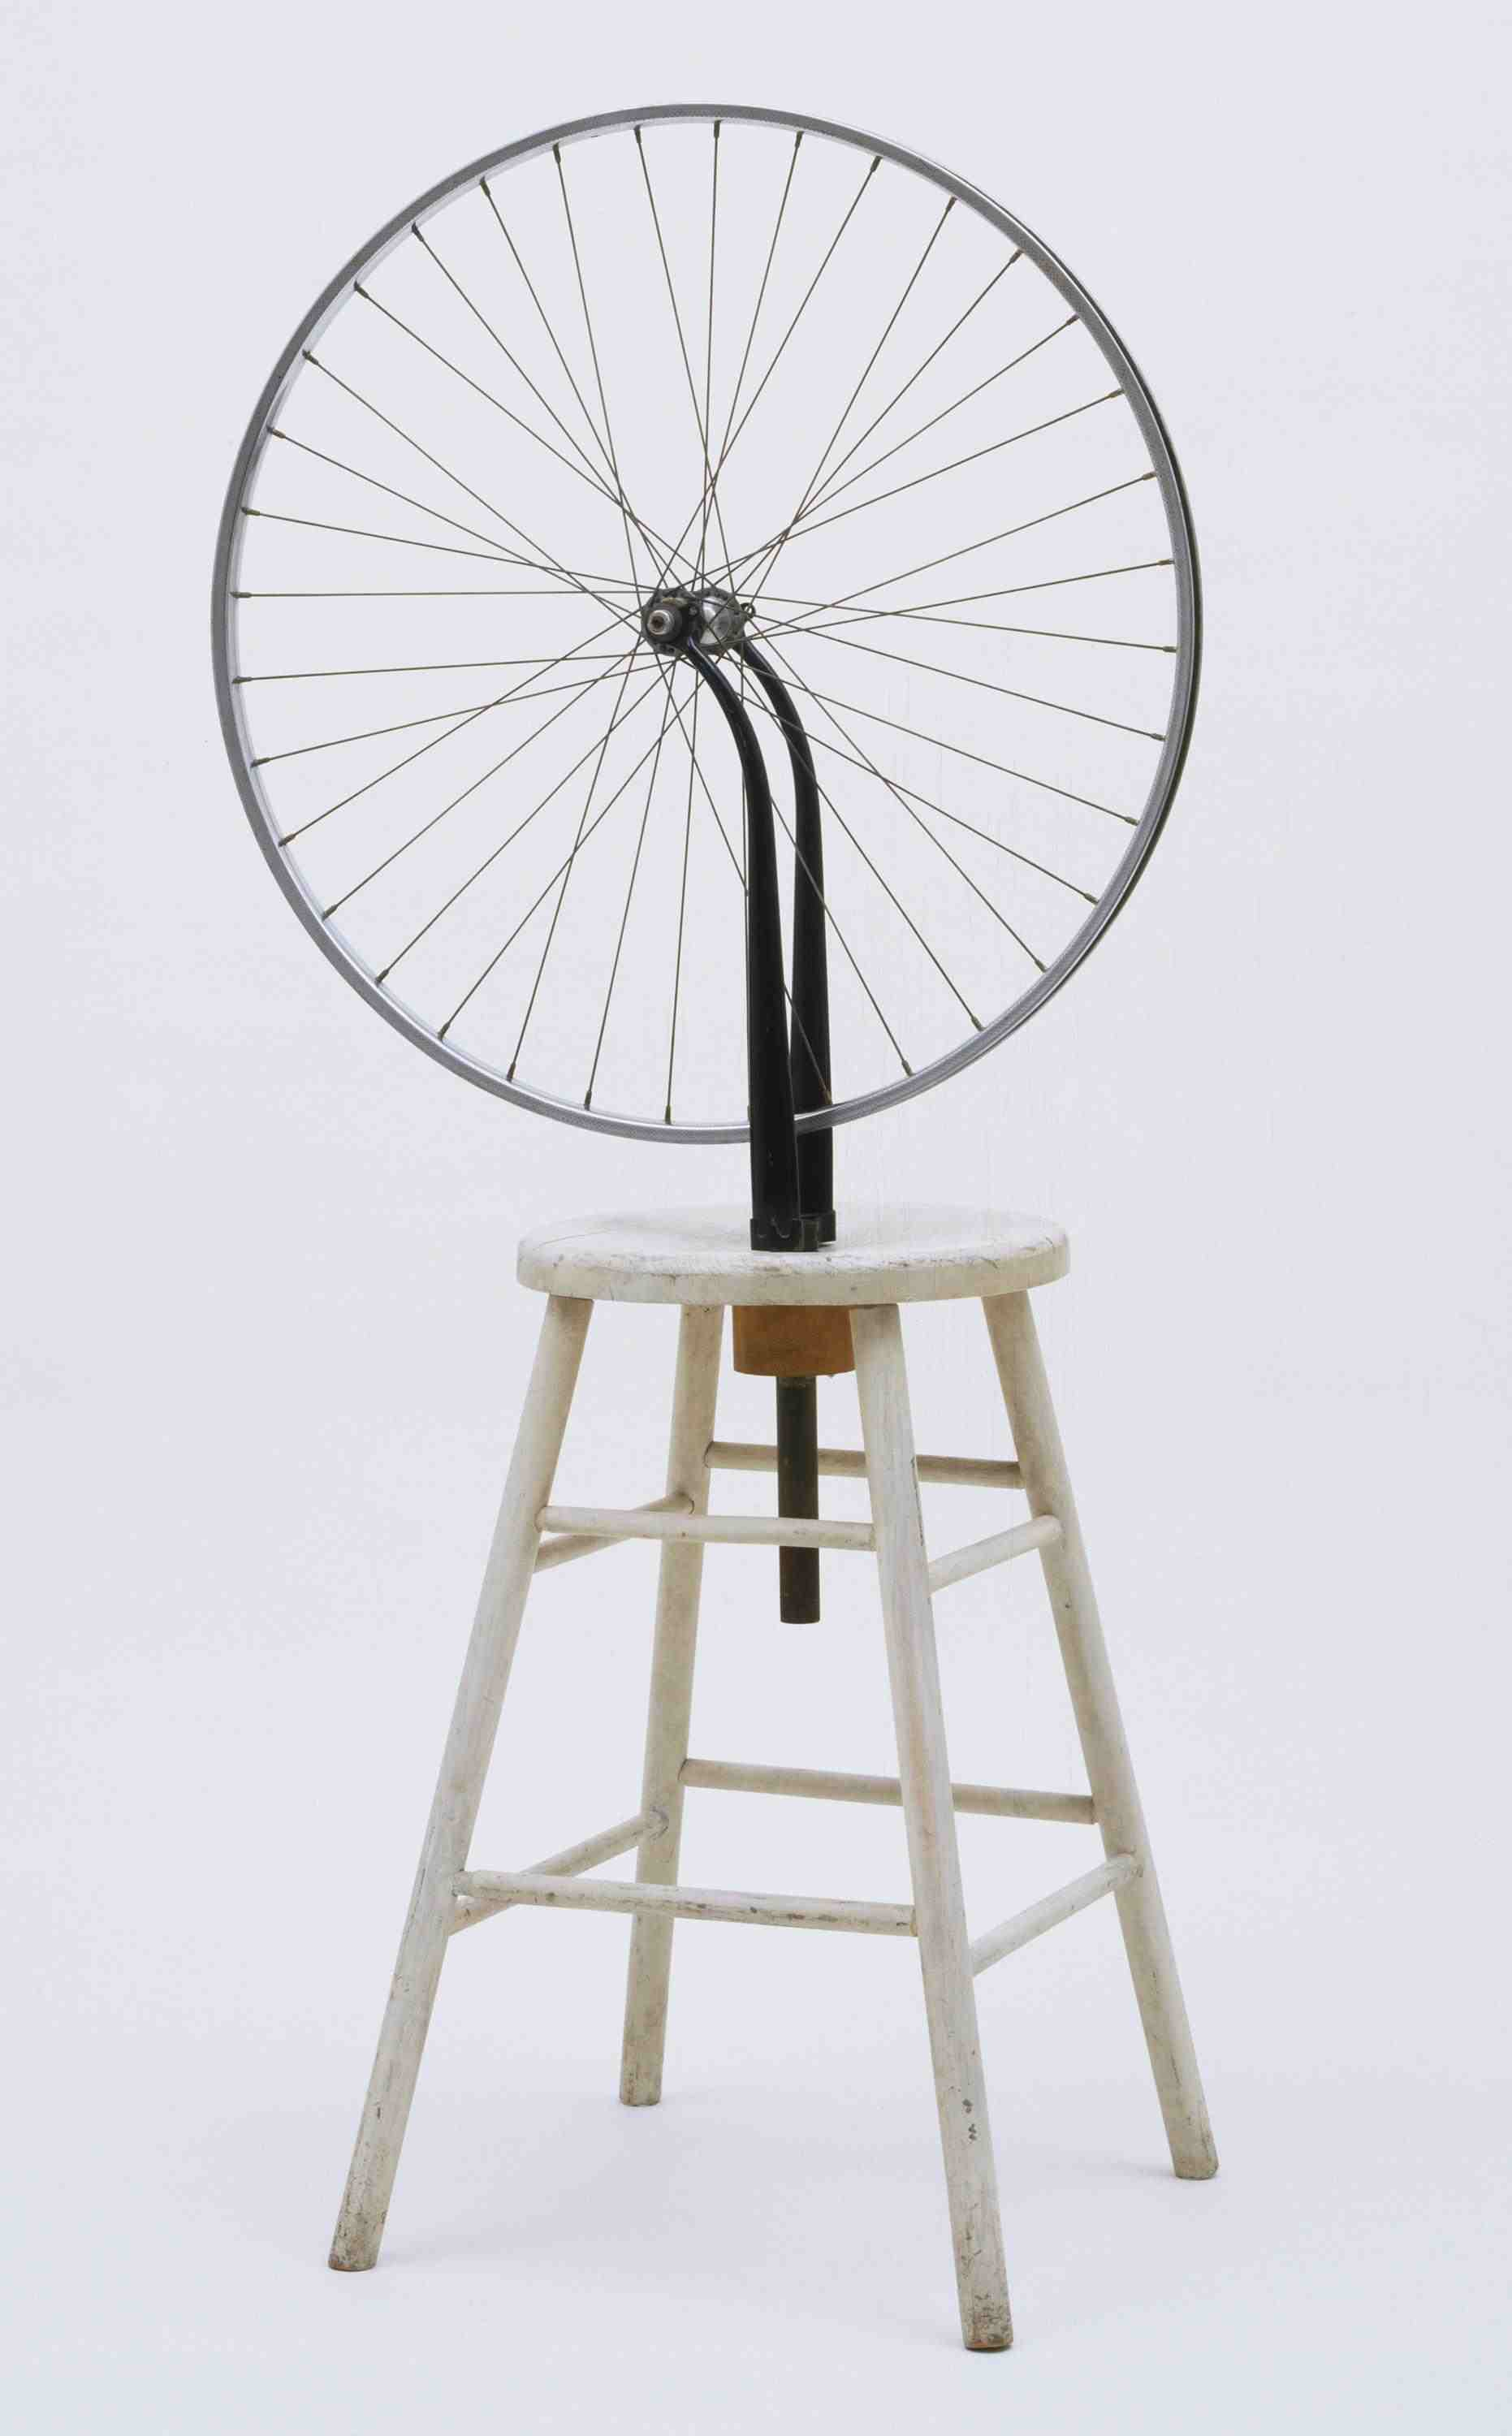
\includegraphics[height=6cm]{graphics/duchamp-bicycle-wheel-1913.jpg}
  \caption{Marcel Duchamp, \textit{Bicycle Wheel}, 1913 (authorised reproduction 1951)}
  \label{fig:Duchamp_BicycleWheel}
\end{figure}

% Found Object
Found object originates from the French \textit{objet trouvé}, describing art created from existing, but often modified, artifacts or products that are not commonly regarded as art, often because they already have a non-art function. They are generally picked up somewhere and their value for the finder might be aesthetic, symbolic and remembrance. \citet[170]{gascoyne1936short} by analyzing found objects in Surrealist art, writes that artist \quotes{discovers a hidden symbolic significance in the [found] object which is preserved when the object is \singlequotes{framed} as art.} In other words, the finder discovers an unrealised significance by removing found object from its previous context and placing it in a new one. The meaning of material artifacts was derived from their symbolic relation to another entities such as person, time, place, experience rather than through their physical attributes \citep{camic2010trashed}. \cite{camic2010trashed} notes that people’s motivation and usage of found objects also occur in various ways. Further enjoyment through found objects is different than appreciating art in museums which is isolated and refined activity. On the other hand discoveries through found object might happen anywhere at anytime. Hence it is not boundaried activity and spread through the daily life.



%****************************************
\section{Examples from Contemporary Artists}
In the light of discussions at previous section, some of the main strategies and approaches of artist are analyzed here. In this section focus will be shifted to the examples from contemporary artists. First one is related with found objects

Photo booths are machines that place crowded places and with affordable cost people can get their photos. It is a phenomena that attract attention of artist and researchers such as Martin Parr and Gerry Badger who published history of them as two volume.

In the French film Amélie\footnote{Original title: Le fabuleux destin d’Amélie Poulain, in english: The Fabulous Destiny of Amélie Poulain} directed by Jean-Pierre Jeunet in 2001, young male character collects photos that are torn up and thrown away by their owner near photo booths spread through train and metro stations of Paris. He collects them and glue them together in a photo album. In the film photo booths and found photos are centrally catalytic. Amélie falls in love with him when she realize him searching for found photos. After his photo album passed to Amélie, she looks every page of photo album again and again. Through the images of unknown people, she establishes narratives that point out the significance of these images even if they are thrown away. The important part of the film, images of a man are generated who scavenge the photos of another people. There are a lot of artist who collects discarded items but their process is not well documented. Therefore we are not fully aware of their artistic process. 

\begin{figure}[h!]
  \centering
  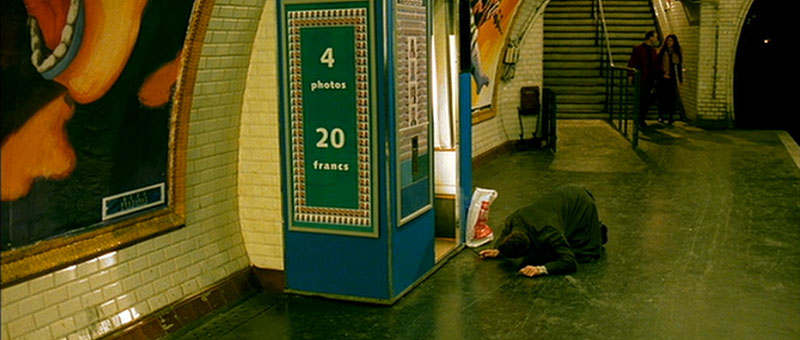
\includegraphics[height=6cm]{graphics/amelie_01.jpg}
  \caption{Still image from Amélie by Jean-Pierre Jeunet}
  \label{fig:Amelie}
\end{figure}

Prior to film Amélie, British artist Dick Jewell published a book in title of \quotes{Found Photos} in 1977. It is a collection of photo booth images that had been thrown away or torn up by the people in the photos. \cite{walker2010dick} comments on that it is \quotes{always a joy to look through.} Images capture diverse range of activities and expressions of people using photo booth machine. They are scavenged by the artist from the photo booths of London. The reasons of why photos are rejected vary including technical problems like flash or posing time. On the other hand, some of them are very good condition, and it is a mystery that why they are rejected. Walker explains that the:

\begin{quote}
gap between our exterior perception of the image and what must have been the internal dissatisfaction of the original subject results in some of the effective moments in Found Photos, where the images are not only bizarre and wonderfully funny (as many of them are) but also profoundly moving.
\end{quote}

Walker argues that even if photo booths are mechanic and simple application of photography while capturing everyday life, leave behind such ambiguous and mysteries that some people trace them. \quotes{Dick Jewell’s approach with Found Photos was less interventionist, presenting the images themselves in the spirit of either an anthropologist showing his finds or a conceptual artist claiming bits of the real world as ready-mades.} His mode of discovery includes climbing to look at the top of the photo booths and looking for the nearest waste bin. Badger describes Found Photos as \quotes{both a conceptual artwork and a sociological footnote.}

\begin{figure}[h!]
  \centering
  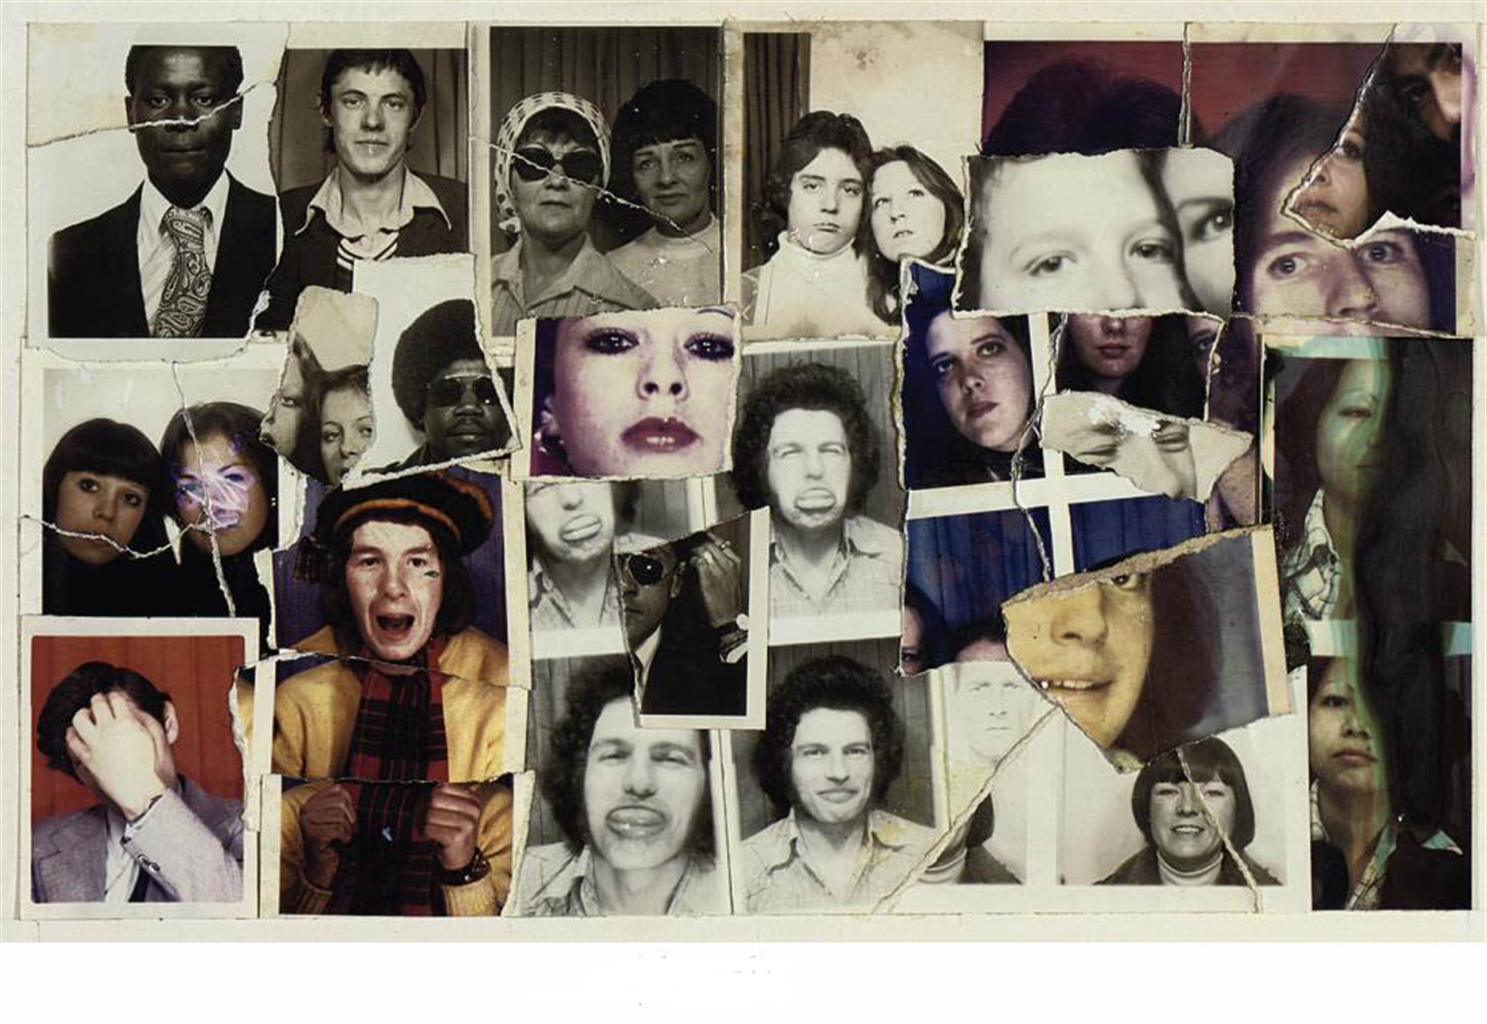
\includegraphics[height=6cm]{graphics/DickJewell_FoundPhotos.jpg}
  \caption{Dick Jewell, \textit{Found Photos}, 1978}
  \label{fig:DickJewell_FoundPhotos}
\end{figure}

On the other side for another artist photographs serve a function to record his daily trash. Tim Gaudreau photographed every object that he threw away for one year. At the end around five thousand images are covered all the gallery and opened to visitors. He notes that it just started as a documentation of his discards, but later it became (part of his life and) an obsession that he can not able to easily quit off. He says that \quotes{this collection of images intimately displays what I do, what I consume. It reveals me.} Like in the case of Tracey Emin trash turns to a medium that is used to express oneself. People are not only composed of the listed items in the CVs, economical power like pointed out in the book (and also film) Fight Club Tyler Durden draws attention to the narrator by saying: \quotes{You are not your bank account.} It is an effective way of looking things left behind rather that things put forward. Through this project, artist reached better understanding what he is and notes that this project changed his consumption choices and patterns.

\begin{figure}[h!]
  \centering
  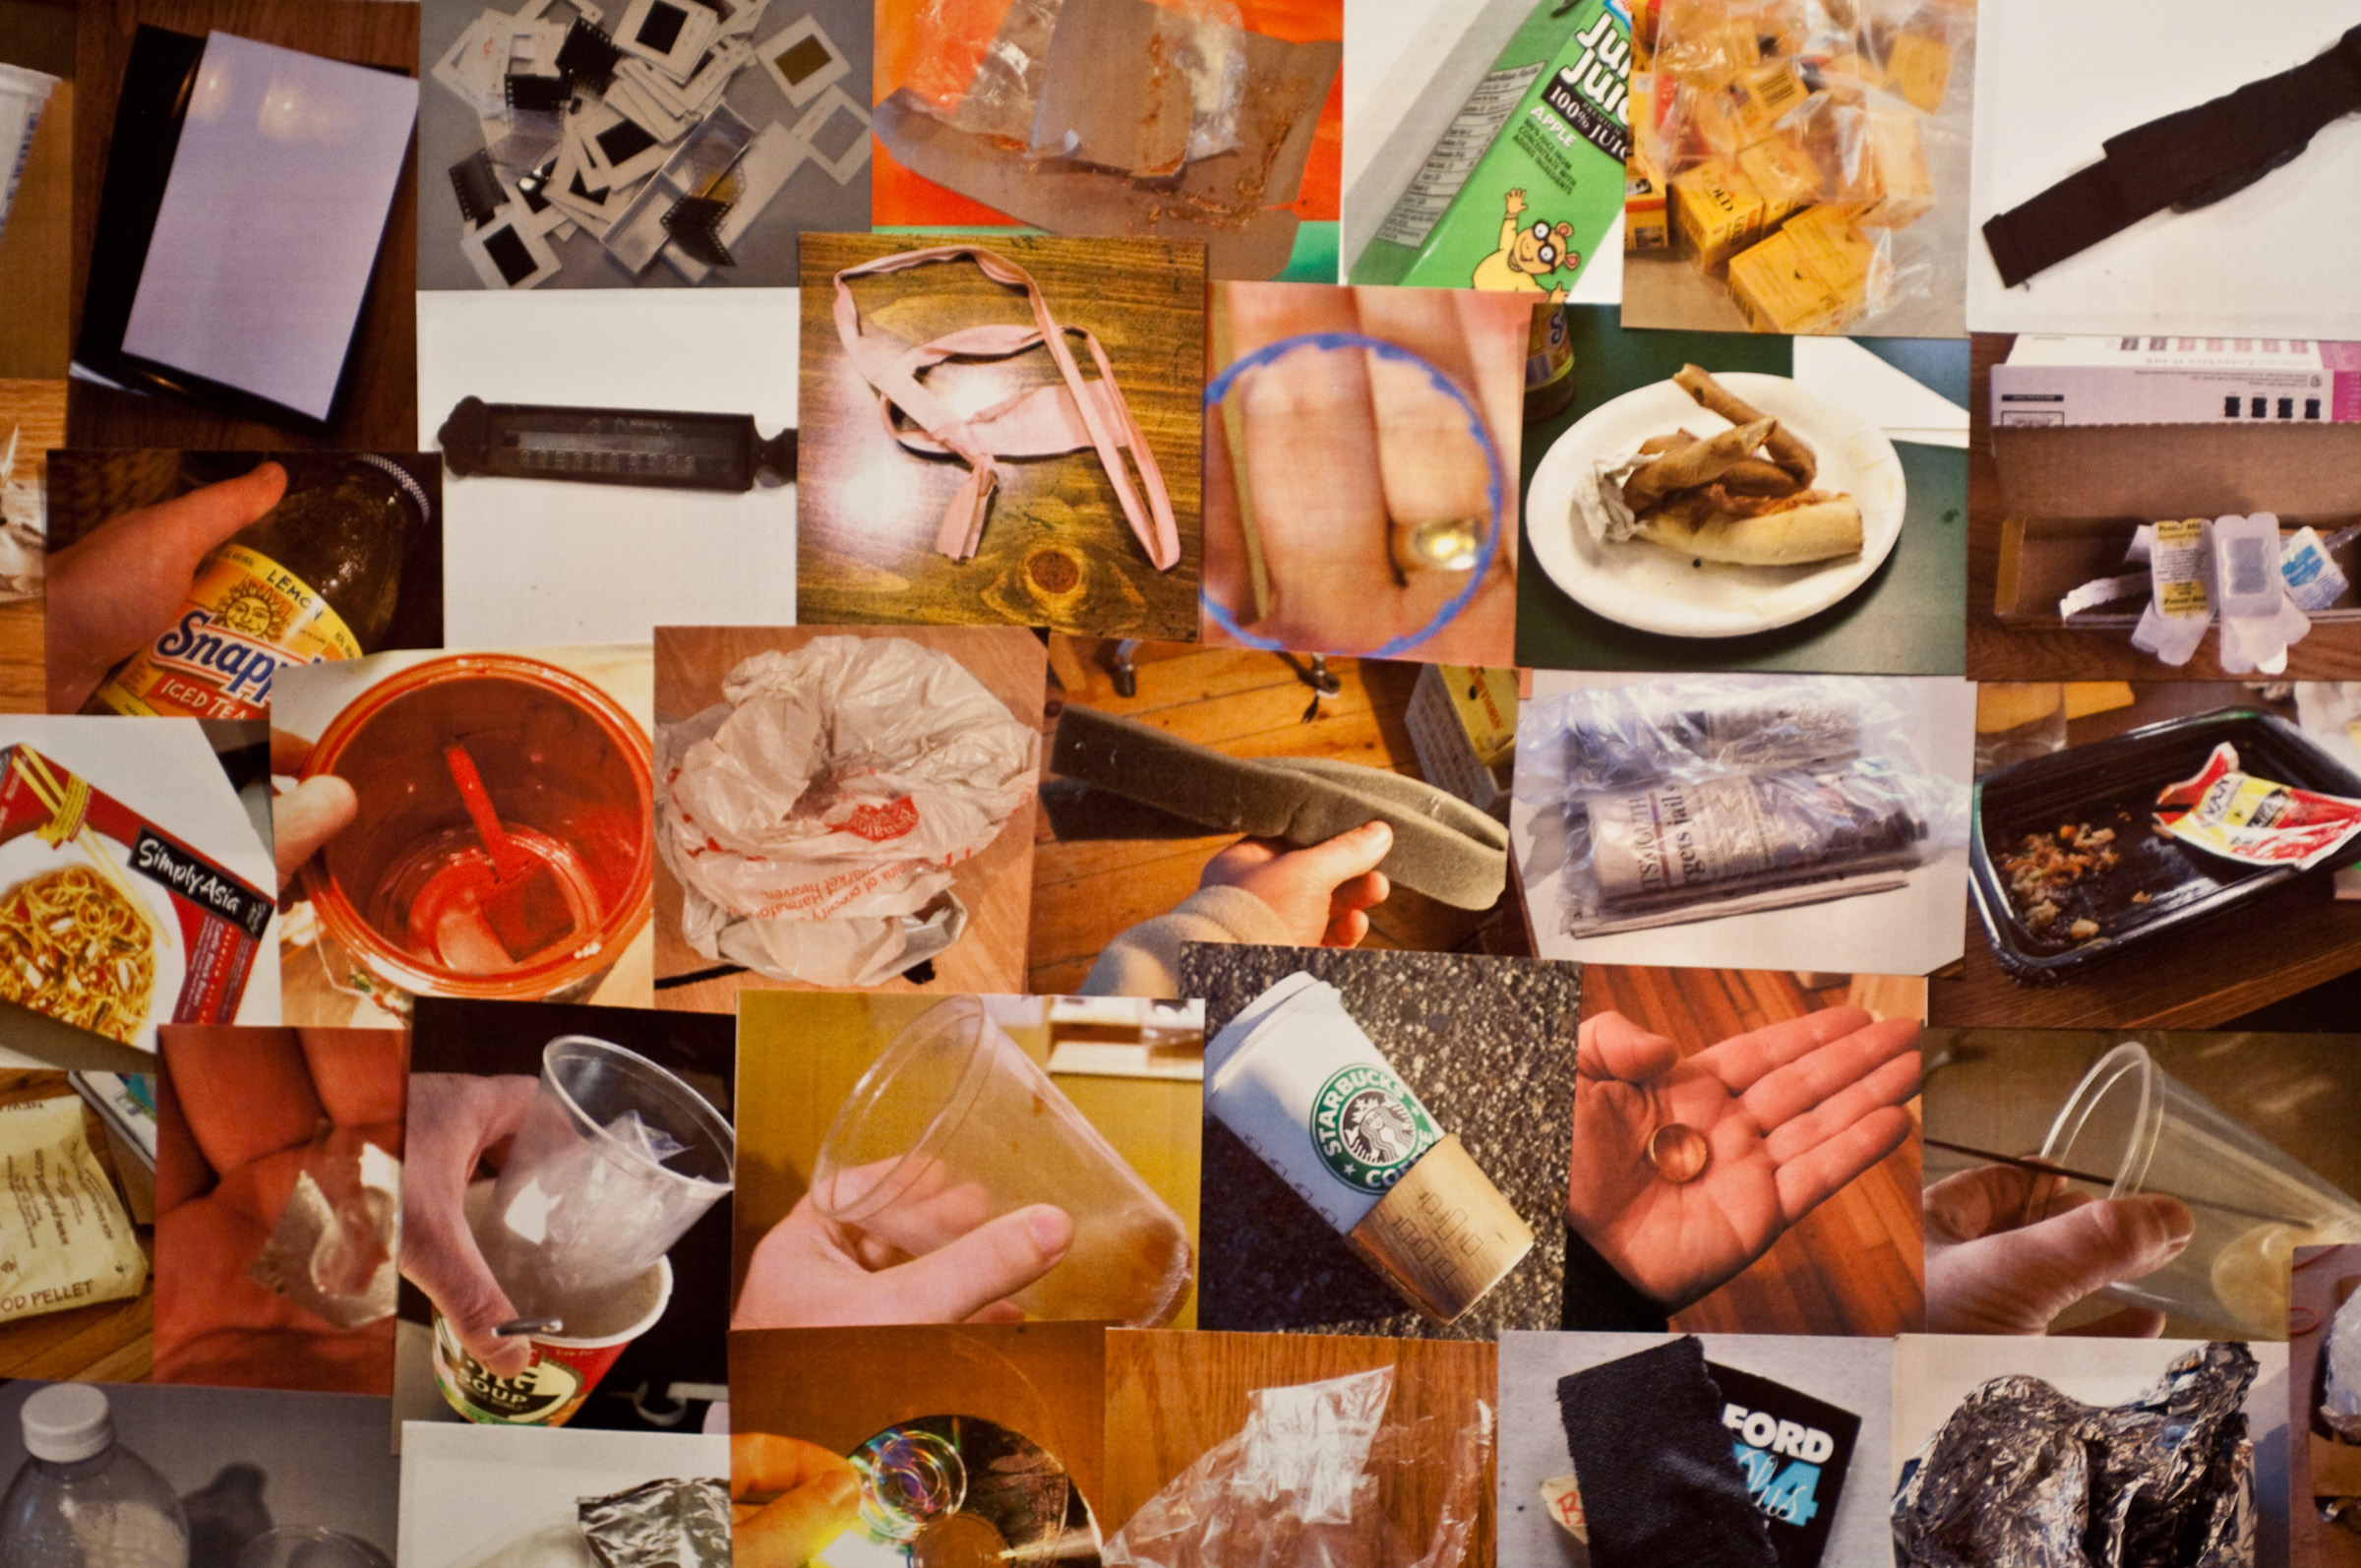
\includegraphics[height=6cm]{graphics/TimGaudreau_SelfPotraitRevealedByTrash.jpg}
  \caption{Tim Gaudreau, \textit{Self-Portrait as Revealed by Trash: 365 days of photographing everything I threw out – Variation I}, 2006, Photograph}
  \label{fig:TimGaudreau_SelfPotraitRevealedByTrash}
\end{figure}

Filomena Cruz turns her lens to the city and its trashes that are left behind, thrown away and squeezed on the sidewalk or pavement. In her photographic series \textit{Road Kill}, she captures tiny trash corpses that are generally ignored and out of sight. In other words, the skin of city revealed through her photos in micro scale. On the skin of city there are lots of trash including \quotes{a piece of chewing gum with an engraved leaf; a flattened-out tube; a corroding paper napkin with a still intact heart; or a frog-green Crayola melting in the heat, all speak the language of \singlequotes{worthlessness} suddenly becoming meaningful} as looked through the window of they capture the city life and skin of the city that we touched. She shows us tiny details of huge cities. Somehow these trashes for all effort succeeded to stay in the towns. These trashes can not be removed from the city but moved ones are stacked on landfill, and they are not tiny as they are.

\begin{figure}[h!]
  \centering
  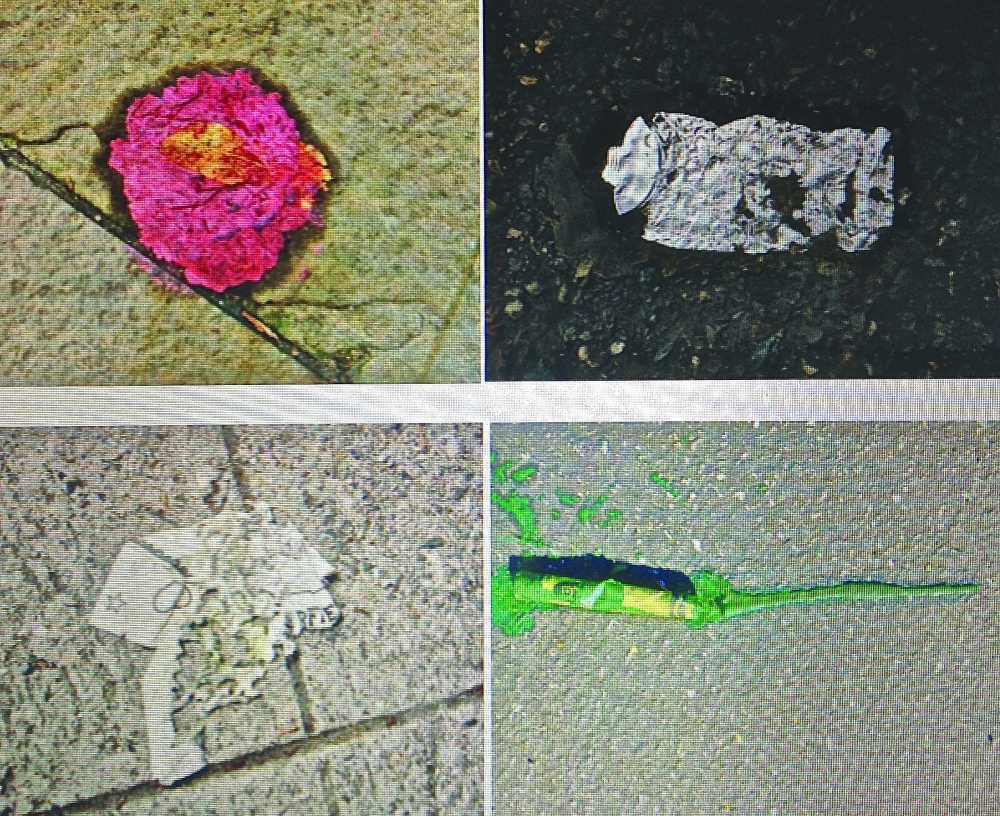
\includegraphics[height=6cm]{graphics/FilomenaCruz_RoadKill_ReVista.jpg}
  \caption{Filomena Cruz, \textit{Road Kill}, 2014, Photograph}
  \label{fig:FilomenaCruz_RoadKill_ReVista}
\end{figure}

In the documentary film, Waste Land, Vik Muniz frames portraits of \textit{catadores} who are pickers of recyclable materials on the dump. He visits them at one of the biggest open-air garbage dump outside of the Rio de Janeiro home of the millions of people. Film documents whole process of development and production of \textit{Pictures of Garbage} made of collected trash from dump. He selects unusual materials and people for portraits rather than the powerful and notable people as commonly encountered at Renaissance. To create portraits of \textit{catadores} there is any other material than trash because of they are already build up their life in trash of city. Also these images are sold an auction and earned money donated to the \textit{catadores}. The images of trash moved to beloved places such as homes and museums. As stated in the rubbish theory they transformed to a durable object.

\begin{figure}[h!]
  \centering
  \includegraphics[height=10cm]{graphics/vik_muniz_marat.jpg}
  \caption{Vic Muniz, \textit{Marat}, 2008, mixed media, }
  \label{fig:VicMuniz_PicturesOfGarbage}
\end{figure}

Not only monumental portraits are extracted from the dump but also an orchestra is grounded up from the dump of Paraguay pioneered by Favio Chávez and Nicolás Gómez. Favio Chávez is a music teacher, and Nicolás Gómez is a garbage picker. They live in Cateura at Paraguay. It is a one of the poorest villages where people live among the sea of garbage. \quotes{A violin is worth more than a house here,} says Favio Chávez by pointing out their hard conditions. Favio Chávez director and founder of the orchestra whose instruments such as violins, flutes and cellos are built from collected trash by Nicolás Gómez. Players of the orchestra are compiled from the children who are hopeless for their future. In the middle of such an existence, these people and musicians have created something both special and truly awe-inspiring. They are given birth to an orchestra that plays the masterpieces of classical music composed by Mozart, Beethoven, and Vivaldi. Trash turned to treasure and totally ironic that a signifier of high culture like classical music can be even played with imperfect instruments. For them and also, most of the people it is not affordable to buy an instrument and get the education of classical music. What they create is actually not expected from them, and their success is not limited with their location. They have given concerts around the world and their motto is: \quotes{The world send us garbage. We send back music.}

\begin{figure}
  \begin{subfigure}[b]{0.48\textwidth}
    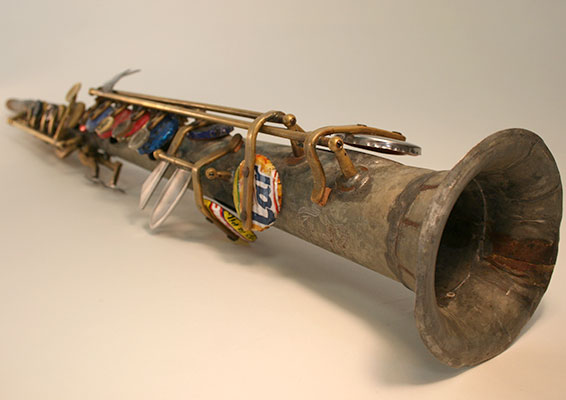
\includegraphics[width=\textwidth]{graphics/landfill_harmonic-sax.jpg}
    \caption{Sax}
    \label{fig:landfill_harmonic-sax}
  \end{subfigure}
  \hfill
  \begin{subfigure}[b]{0.48\textwidth}
    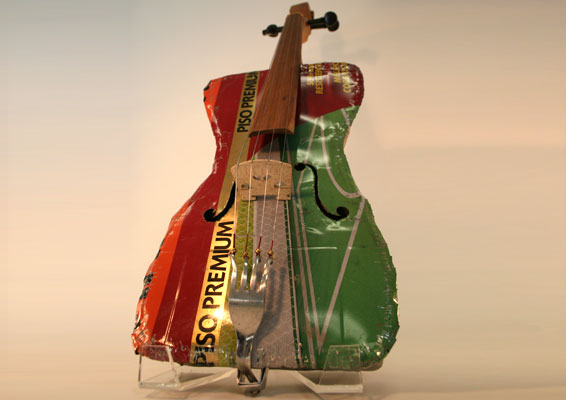
\includegraphics[width=\textwidth]{graphics/landfill_harmonic-violin.jpg}
    \caption{Violin}
    \label{fig:landfill_harmonic-violin}
  \end{subfigure}
  \caption{Instruments of Recycled Orchestra}\label{fig:animals}
\end{figure}

As noted that recycling is an economic strategy of survival in developing countries throughout the world \citep[25]{cerny1996recycled}. Creative production that is motivated, primarily, by adverse conditions of economic necessity. Economic survival and adaptation are influential factors for both the makers, who build an informal business on the making and selling of recycled goods and the local consumers, for whom the market for affordable, utilitarian goods is devised. 

Nicolás Gómez builds musical instruments from what is available for him, in this case it is rubbish. His practice and works can be seen as an example of \textit{bricolage}. Dictionary meaning of it is something constructed by using whatever is available at hand. The French word \textit{bricoleur} is someone who works with own hands and construct \textit{bricolage}. The term coined by \citet[17]{levi1966savage} and he explains it as:

\begin{quote}
[He or she] is adept at performing a large number of diverse tasks; but, unlike the engineer, he [or she] does not subordinate each of them to the availability of raw materials and tools conceived and procured for the purpose of the project. His [or her] universe of instruments is closed and the rules of his [or her] game are always to make do with whatever is at hand, that is to say with a set of tools and materials which is always finite and is also heterogeneous because what it contains bears no relation to the current project, or indeed to any particular project, but is the contingent result of all the occasions there have been to renew or enrich the stock or to maintain it with the remains of previous construction or destruction. 
\end{quote}

In the scope of painting different than the works in the previous chapter (paintings on tea bags and coffee cups) historical portraits of notable people are painted onto the flattened aluminum drink cans which are disposable objects. The people in the figure \ref{fig:Alsbrooks} is General Jefferson C. Davis who was an officer at United States Army in 19th-century. Selected persons can be viewed as a member of the higher or ruling class of society. Therefore Kim Alsbrooks, painter of these works, might have thought that to make trash is more valuable, their face will be good or vice verse. She probably use trash to criticize social elite of that time. 

\begin{figure}[h!]
  \centering
  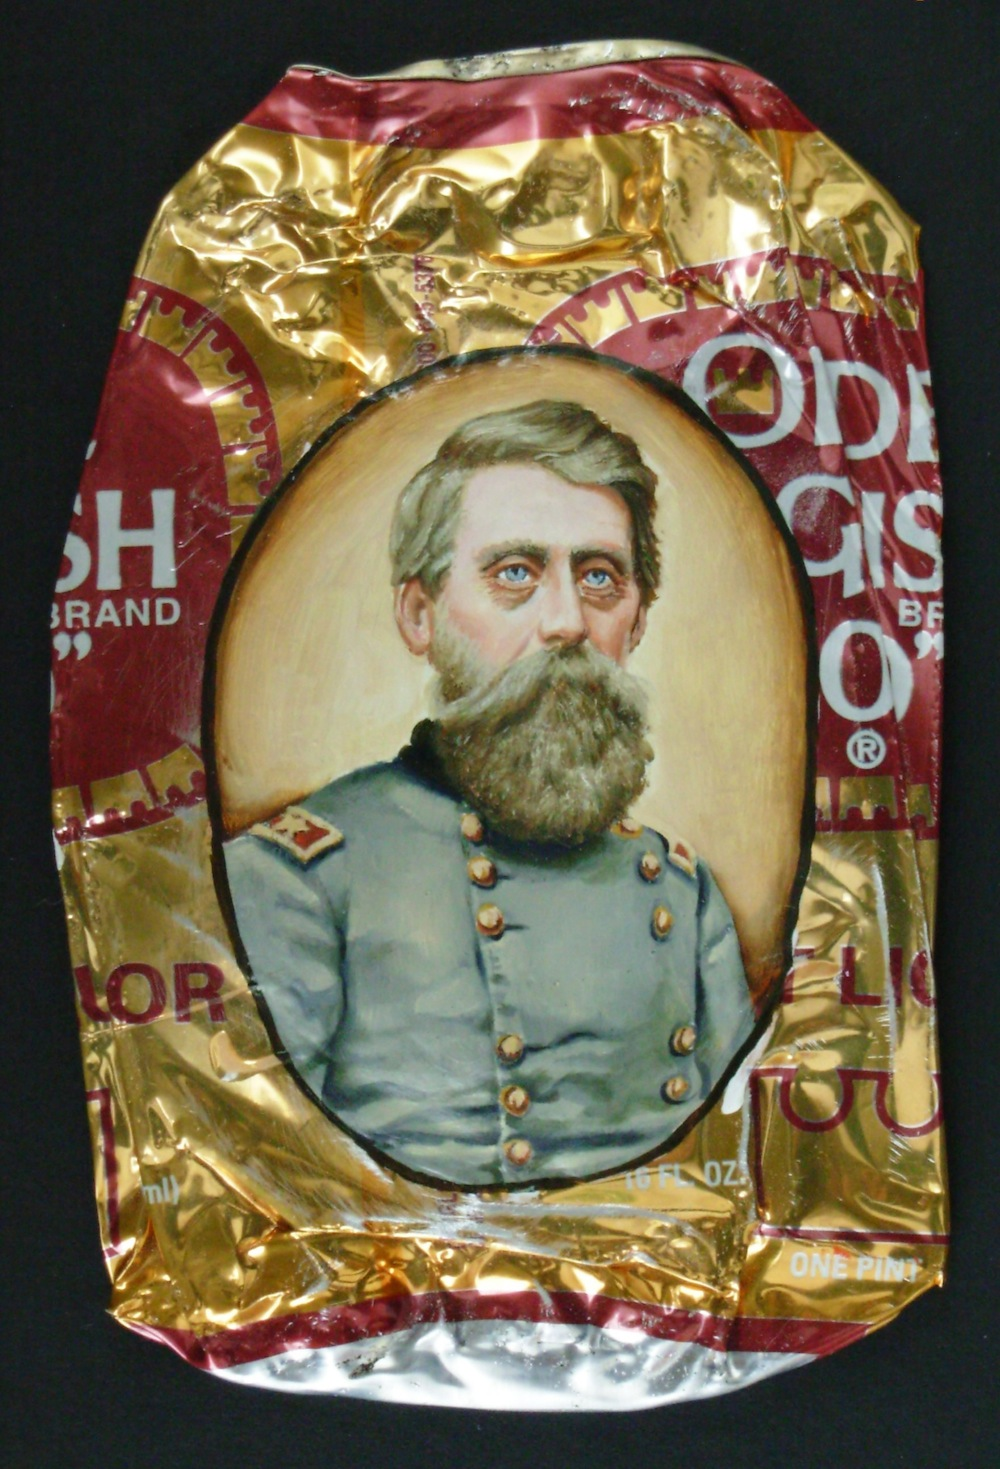
\includegraphics[height=8cm]{graphics/Alsbrooks.jpg}
  \caption{Kim Alsbrooks, \textit{Gen. Jefferson Davis}, 2015, oil on aluminum can}
  \label{fig:Alsbrooks}
\end{figure}

Not all the time and every artist turn trash into different objects, sometimes they only trash them. Michael Landy’s Art Bin is one of them. It is a room size transparent bin placed inside of the art gallery. He invites people to bring their own artworks of failed attempts. Some of the notable contemporary artists such as Damien Hirst, Gillian Wearing, Tracey Emin and Mark Titchner participated in by throwing their sculptures, paintings, and prints into the Art Bin. People publicly toss their work from a high platform, and all of them can be seen outside of the transparent walls. He listens to the story and the failure of the artworks from their creator, and it is not allowed to throw others work. At one side he criticizes the idea of not aware of that artist also have lots of failures. People only can see the final work in the galleries and museums. In this work he break-ups this notion that encouraging the artist reveals their failures to the public. Like his words, it is \quotes{a monument to creative failure.} On the other side, there is a provocative approach to the art and art objects by saying that \quotes{Nothing is too good for the art bin.} There is no limitation of throwing away even if art. 

\begin{figure}[h!]
  \centering
  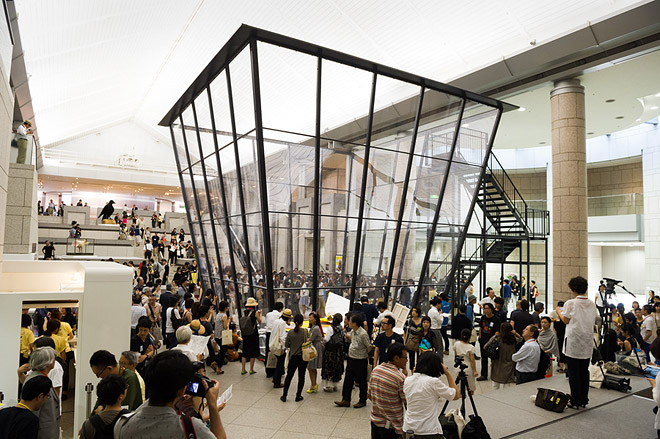
\includegraphics[height=8cm]{graphics/MichaelLandy_ArtBin.jpg}
  \caption{Michael Landy, \textit{Art Bin}, 2014}
  \label{fig:MichaelLandy_ArtBin}
\end{figure}

Not all artist transform trash although some deconstruct them. Michael Landy is one of them. Michael Landy’s Break Down Inventory is a two-week show (display) of destruction process of his all possessions on a dissemble line with the help of 10 workers. Firstly they are classified and recorded for three years and the deconstructed in two weeks by separating every element to the smallest part. Reveal all his possessions and deconstruct of them while he is alive. He turns them to rubbish and makes them unusable. Breaking down the all the meaning. Breaking down the connections. It can be an example of a downcycling process. It is preferred to decompose all the complex link and relationships between the objects. They are not just ordinary things they are possessions of the artist. Break Down 2001, in which he systematically destroyed all his personal possessions. His work examines what we value and what we discard, consumerism and waste, and human labor and its worth. It happens in public space. People can see the process. This process lasts two weeks at a place where people buy goods.

\begin{figure}[h!]
  \centering
  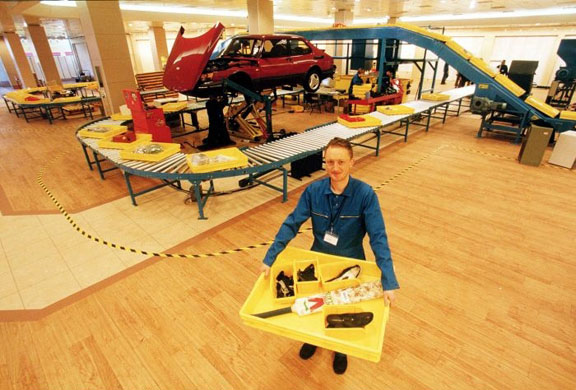
\includegraphics[height=7cm]{graphics/MichaelLandy_BreakDown.jpg}
  \caption{Michael Landy, \textit{Break Down}, 2001}
  \label{fig:MichaelLandy_BreakDown}
\end{figure}

The film American Beauty, which features a long, poetic clip of a plastic bag swirling on an eddy of air yet people find it hard to think of plastic bags as things of beauty. However, as a product --as something created and then unleashed to become seamlessly integrated into the lives of millions of people around the world--- there is a strange allure to them, just as a pathologist can admire the structure of a particularly virulent and contagious virus.

% TODO burayı da düzeltmek gerek.
Examples are not limited with these. Even if \quotes{trash is dirty and smelly trash can provide the raw materials for exquisite art---from sculpture to film and beyond.}



%
\section{The Documentary \quotes{The Gleaners and I} by Agnès Varda}
\quotes{The Gleaners and I} is a French documentary film directed by Agnès Varda in 2000. The film emphasizes diverse types of gleaning from rural to urban. According to the Merriam-Webster dictionary gleaning refers \quotes{to gather grain or other produce left by reapers}. Varda searches for the historical and current practices of gleaning in rural and urban areas of France. Historically, gleaning is the act of collecting what is left and not profitable crops after the harvest. By combining different fragments through his film, she shows that the act of gleaning also exists in various forms and styles. In particularly she curiously focuses on the (un)familiar people who glean leftover of society. Moreover, it is a self-reflexive film because the director establishes a relationship with the practice of gleaners and her film making practice. Some people glean crops; the others discarded food, and Varda gleans images.

The film is more than a research and document of the lives of many gleaners. It highlights the degree of global consumerism of the modern world and how technological advancements (or industrial (technical, modern) standards) result in waste. Varda seeks the several stages of potatoes from producers to consumers. As she discovers that supermarkets buy only potatoes that fit in industrial standards of shape and size. So what happens to the others? Varda discovers and shares with us the disturbing fact that they are taken back to the field where they came from, by following with the camera the trucks that unload mountains of potatoes. As Rosello notes that \quotes{The \singlequotes{good} potato is not the edible potato but one that will fit into a plastic container to be displayed on the shelf of a supermarket.} Varda records few people who glean the rejected potatoes from the field, and also she joins them by collecting heart shaped potatoes that fascinate her. Rosello explains that she is collecting not only refused potatoes but also images that are left behind.

\begin{figure}[h!]
  \centering
  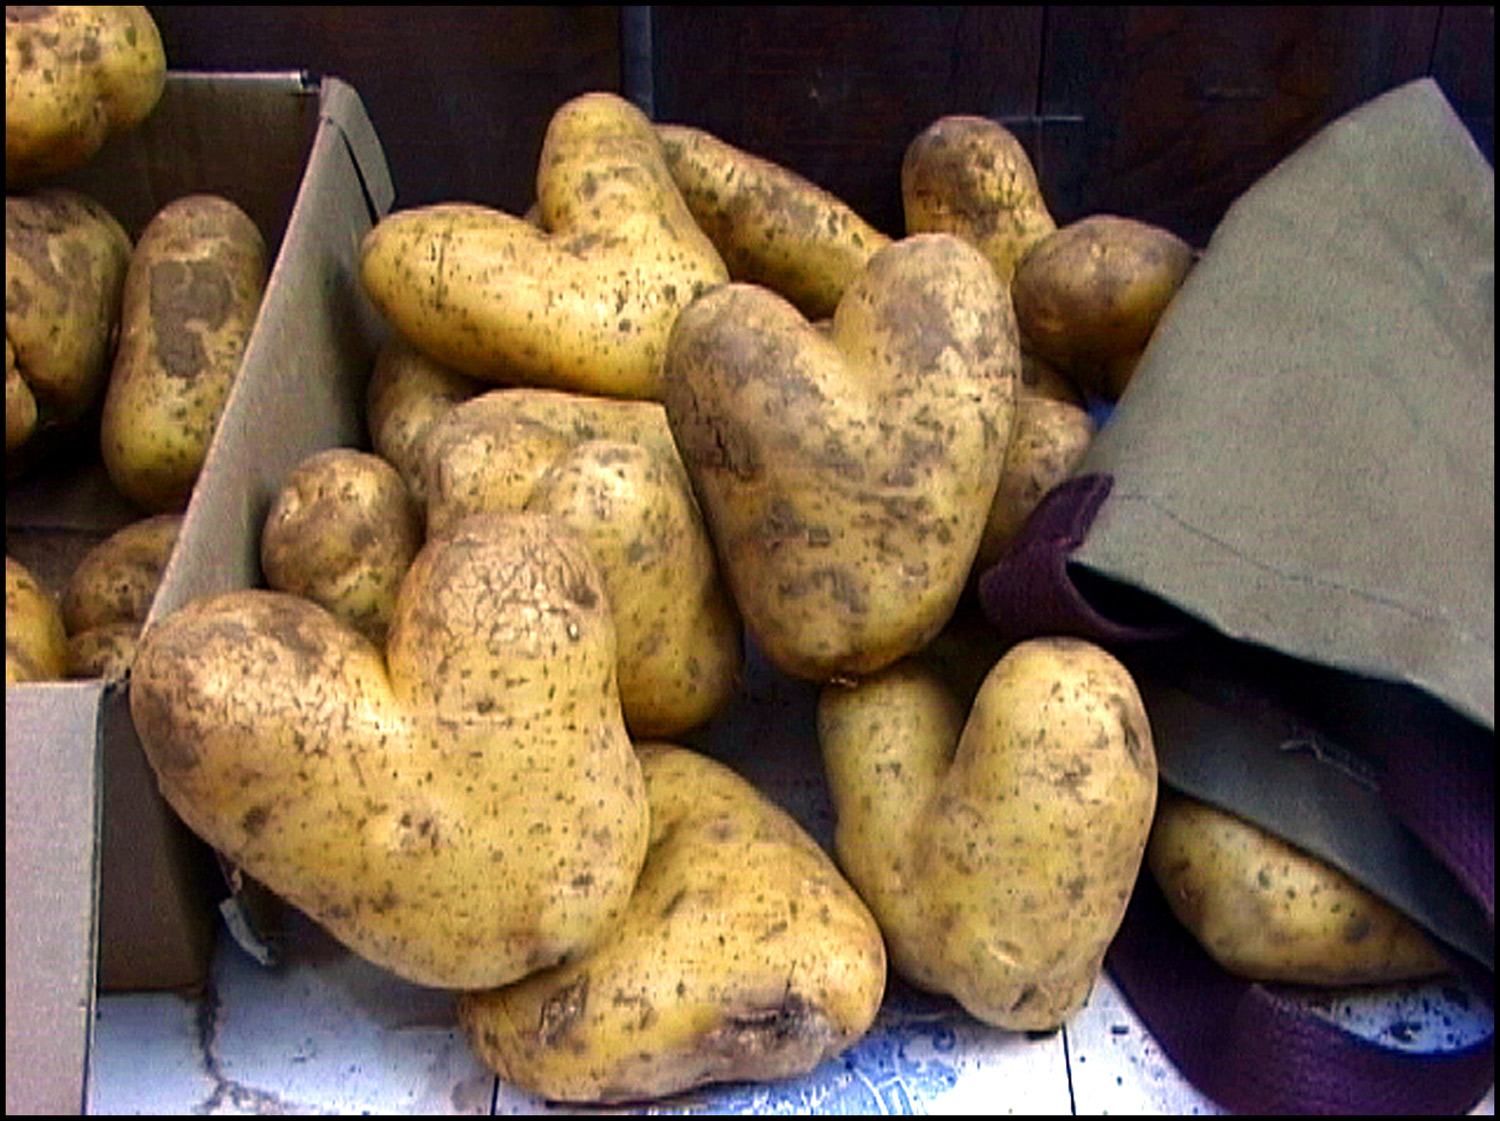
\includegraphics[height=6cm]{graphics/AgnesVarda_Potatoes.jpg}
  \caption{Still image from The Gleaners and I}
  \label{fig:AgnesVarda_Potatoes}
\end{figure}

The industrial processes have some standards and beyond that standards, there is not a place for anything. It clears out (or move away) the rest. It can be viewed as the idealization of goods and products (even people). At this point, it can be referred back to Žižek’s claim that people’s false consciousness about balanced and idealized notion of nature. It can be understood that this type of clarification of objects may result in this false perception. What Varda’s finding is an excellent exemplification of what Žižek wants to point out.

Contrary to the common act of discarding, Varda finds out a creative way to use her unconscious recorded piece that might be deleted by the others. It is the scene where Varda had forgotten to turn her camera off and accidentally films the ground and her lens cap bouncing along as she walks. She uses this scene with a jazz soundtrack at background. Watching this scene is confusing at first hand regarding context. It might be viewed as worthless and recorded by accident. One can ask that why is this placed here, what does this have to do with gleaning? However, Varda forces us to watch it (wants us to pay attention). This scene called as \quotes{the dance of the lens cap.} Ruth Cruickshank in the article, The Work of Art in the Age of Global Consumption: Agnes Varda’s \textit{Les Glaneurs et la glaneuse} (The Gleaners and I), addressed this scene and clarified the potential deeper meaning behind it. Cruickshank likened the scene to something that is normally thrown away, or in this case edited out of the film, much like the way trash is thrown away or food is left behind after a harvest. \quotes{Where many documentary makers would leave such accidental footage on the cutting room floor, Varda draws attention to how what would habitually be perceived as waste may be viewed as supplement with its own intrinsic value. Rather than literally treating it like dirt, Varda retains and prompts reassessment of that which is normally left out of shot} \cite{cruickshank2007work}. Things that are often forgotten or discarded can easily be revamped to create something useful to someone. The scene was revamped using music, and it became beautiful, much like the gleaners who found fish in the trash cooked it to make it edible, or the artist gleaner who piled discarded baby dolls into totem poles.

As Varda indicates, people can be found throughout the French countryside gleaning everything from apples to oysters, potatoes to grapes, much as they did hundreds of years ago (though no longer in organized groups). Making use out of something that has been left behind and labeled as obsolete is not unique to potatoes. There is so much discarded, yet still-viable food in dumpsters that many people live off it entirely. More metaphorically, there are also urban gleaners who scavenge scraps from bins, appliances from the side of the street, or vegetables from stalls after the markets have been closed. By showing them she explores that once was a common practice of gleaning throughout the years has evolved, but not disappeared. She keeps light to the modern life gleaners that are not visible every time. One of them is the teacher named Alain, an urban gleaner with a master’s degree who teaches French to immigrants and refugees who are also considered as surplus of society. It can seen that from this example, gleaning becomes also a form of resistance to ruling system ---a way of rejecting to be limited by mainstream expectations and lifestyle.

She shows that the act of gleaning does not bound to the collecting food and survival reasons. Some of them build their own meaning, existence and identity through the collected items. One of the examples that she gave is that the man who collects baby dolls and use them in the decoration of his home. Every where is filled up with the baby dolls even if the wall of the garden.

Through the film she experiences the act of gleaning with different people. At one side she gleans potatoes in the field and on the other side follows a man with bicycle look for the garbage in front of the homes. By documenting their life in action she also participates their life. But she brings her own perception to them. For example in the case of potato gleaning she collects the heart shaped ones which attract attention of her. Moreover in the case of night searching, she finds a clock without hand. It has fulfilled its function and left away. Most important part of clock is missing therefore it is not functioning. However for her it has a different meaning. Not every time people seek to be aware of time sometimes they want to forget that.

A clock without hands found the garbage pile and taken by Agnès Varda. It does not work properly but it has important meaning for her. The time does not go on and it does not remind her that she is aging. One of the interesting thing is here Agnès Varda feels that as an aging person who will later become a discarded person.

Here another point is that Agnes records images of people picking up things from the ground like their ancestors. Everyone somehow collect things in their life but particularly she selects these people and their images in action. There should be a reason for this! For some individuals, gleaning is not a novelty or a clever way to save money, but a necessity of life. They require it to sustain their life. Combine the elements from different peoples that seems totally unrelated gains powerful theme for the documentary. What gleaning means become more open (or powerful). It draws a picture of body combination of different parts (connected, dependent to the each other). The reason of gleaning varies but the fact that gleaning is continues in different forms.

She discusses the importance of found in the meaning and purpose of art forms like this: \quotes{Varda seeks to encourage viewers to consider what potential agency is demonstrated in the artfulness and contingency of gleaning by individuals excluded\ldots from the homogenizing systems of global consumption} \cite{cruickshank2007work}. One can find more treasure in trash than many of New York’s finest galleries and art exhibits; they bring a grassroots feel to what has always been seen as a stuffy and prude aspect of society.

She investigates and talks artists who are using discarded items in their works. Which people could not find anything, the artists see countless possibilities. French collage artist Louis Pons is one of them. He specializes in reliefs and assemblages made wholly from refused materials and trash. Pons describes his artistic process and understanding of art as what others see \quotes{a cluster of junk,} he sees \quotes{a cluster of possibilities.} Varda records his studio which contains many scraps, pieces of junk with various shapes and color. Combination of these provide countless representations. By showing these people and their ideas about junk, Varda presents alternative ways to see objects and invites people to rethink. There is always alternative ways to see something different. It is like giving life or finding life from discarded object.

\chapter{NOTEBOOKS FROM TRASHED PAPERS}



\begin{singlespace}
% FROM Wild Art. quote taken from the television series `American Masters', Season 5, Episode 8, John Cage: I have nothing to say and I am saying it (aired on 17 September 1990).
\epigraph{The first question I ask myself when something doesn't seem to be beautiful is why do I think it's not beautiful? And very shortly you discover that there is no reason. If we can conquer that dislike, or begin to like what we did dislike, then the world is more open. That path ---of increasing one's enjoyment of life--- is the path, I think, we all best take: to use art not as self-expression, but as self-alteration; to become more open.}{\hfill---John Cage, \textit{Wild Art}, 2013}
\end{singlespace}





In this chapter thesis project and its development progress will be explained in detail in the light of what has been discussed in previous chapters. The project will be examined in various dimensions. The relationship will be established between the previously mentioned artworks. How this project is related to the discussed concepts and how it can be positioned among the previous works will be explained.

Firstly, brief statement and description of the work is given. Secondly, the development of the project and experiments are explained. Lastly, the final body of the work with its parts is presented.





%
%
% TODO: Be careful on tenses.
\section{The Statement}
Refuse is part of people’s consumption practices. It is a very common concept from developed cities to rural areas, from modern societies to ancient societies. It is not wanted, thrown away, kept away. It is considered as useless, disgusting, abject, unattractive, and harmful to the people and nature. Contrary to the common approach as \cite{thompson1979rubbish}, author of the book Rubbish Theory, stated \quotes{one man's trash is another man's treasure}.

With the collaboration of many people discarded papers and packages were collected from different places. This time, it was not thrown away, it was collected and saved. Later they were transformed to notebooks by hand with traditional methods. Juxtaposition of trashes create notebooks that are different from the blank industrial ones, and through them challenged the widespread understanding of trash.

Through this project trash were re-imagined (re-considered, re-thought), new possibilities and alternatives were seek. As it is discarded, missed potentials were discovered.  This project aims to find new potentials on trash.

The purpose is not to build an object that is produced from discarded material to watch it from distance. The important thing is to interact with it. It is already discarded and general behavior avoid from it. This work must change it. It must call the viewer to interact with it. Trash must be accepted by them. This project asks people to readmit the trash to the their life. For this reason notebooks are given away free at various places where people visit frequently. By doing that once thrown materials would find a place with new purposes in the community.





%
%
\section{Development Progress of the Project}
In order to have an insight of this project and realize artistic intentions, it is important to look at the process that reveals the path to the final work and critical decisions that were necessary to the completion of the project.

Through the process, there are several problems that needed to be solved. Some of the questions in my mind are solved through the research on the subject. Further, the found samples of artworks played significant role in progress. They helped me a lot to shape unclear points of the project. They provide me a deeper understanding of the subject and what I am doing. In other words, they lead me during the development of the work.

% This progress also reveals that how this work can be positioned among the other works.





% NEW PART [approach, history] 
Before explaining the details of the work, it would be better to explain how it was started and what is my approach to the trash.

My interaction with discarded material is not limited with this thesis project. There are a few previous attempts and several memories that I remember. Briefly, I want to examine them. These will also reveal my motivation and approach shaped through time and how thesis work affected from it.

% [SODA CAPS]
I remember from my childhood that we were collecting soda caps and were playing with them. We were looking everywhere to collect them. Some caps were found less and they worth more in the game. We put them on the railways to make them flat. After the train had passed we had perfect flat caps for our games. At that time, it was not waste for us. It has a value and part of our games and indispensable source of fun. The notion of playing with it can be related with the Picasso's collage work \quotes{Still Life with Chair Caning} mentioned previously. He pasted letters of the French word \quotes{JOU} means \quotes{game} signifying that playing with the materials. We were already playing with trash while we were child. Therefore, it can be better understand that why Picasso said that \quotes{every child is an artist}.

% [VASVIYE HOCA]
Another important memory is from my primary school teacher. When I was at third class, our teacher wanted us to bring colorful papers to make something (whatever it is I do not remember now). The day after we brought some colorful paper that was bought from stationery store. Our papers' shape and color looked same. However her papers were different in every dimension. They were cut out from packages and advertisements. I remember clearly that she suggested that same for us. \quotes{Do not throw out packages, look for the useful parts and keep them to use later.} Whenever I am going to throw something away, this comes to my mind. Can it be reused? Every time it is not obvious that how can it be useful, but at some point it becomes an indispensable practice. Further, this practice is also support to the bricolage methodology. Keeping many things makes easier to build (or produce) whatever at hand. 

% [Song Dong]
The main idea is to save them to use later. For some people it is a life saving practice. It can be seen in the case of artist Song Dong's mother (mentioned in chapter 2). This practice result in establishing stronger and intimate relationship with objects. 

I am very uncomfortable with the act of discarding. I often think that by discarding objects, I am missing their potentials. I must find another use which is more effective than throwing away. At least I can give them to someone else who can use it for own purposes. Seeing papers on the waste bin is a disappointment for me. As artist Aaron Kramer argues that \quotes{[t]rash is the failure of imagination} \citep[as cited in][]{meyer2007turning}. There is a lot of effort to produce objects and it seems that all this efforts are wasted. What I mention is not related about ultimate productivity. It is more close to being thoughtful, and taking responsibility of tools, items and objects that we are using. Rather than throwing out, creating a way that all are have chance to live together is much more close to my perception. On the contrary, sometimes I became overwhelmed because of the significant amount of leftover from daily activities and in order to move on I need to leave them behind. It is the result of inevitable rhythm of modern life style. Consuming and wasting is part of people's daily routine and most of the time they are not aware of what they consume, and what they discard. In the scope of this thesis subject, saving objects rather them getting rid of them is an effective way of breaking the routines. The use of that object can be decided in the future. 

% [encouraging point]
One of the encouraging factor of working on trash is to explore something different that others cannot see. In other words, it contains eureka moments. Because it is ignored by discarding and therefore undiscovered. It waits us to be discovered and possibly (as Picasso's explanation on his work 'Bull's Head'\footnote{See epigraph in the beginning of Chapter 3}) discovered again and again. 

% [EXPERIMENTS AT HOME]
My remarkable interaction with trash is from recent years. Long years I stayed at dormitory during when I was high school and university while undergraduate. Dormitory is place that living spaces is shared with many people. Therefore there is a limited place for you and your possessions. There is no space for unused items. After I graduated from university I started to living a rented house. This give me to opportunity to save the materials to use them later. My very first intention is to use them on my painting. Instead of white blank canvas I want to experiment with different surfaces. I collected boxes and cart boards from my friends. My aim is to turn discard materials to the different things. Here is some of the my previous works.

\begin{figure}
  \begin{subfigure}[b]{0.31\textwidth}
    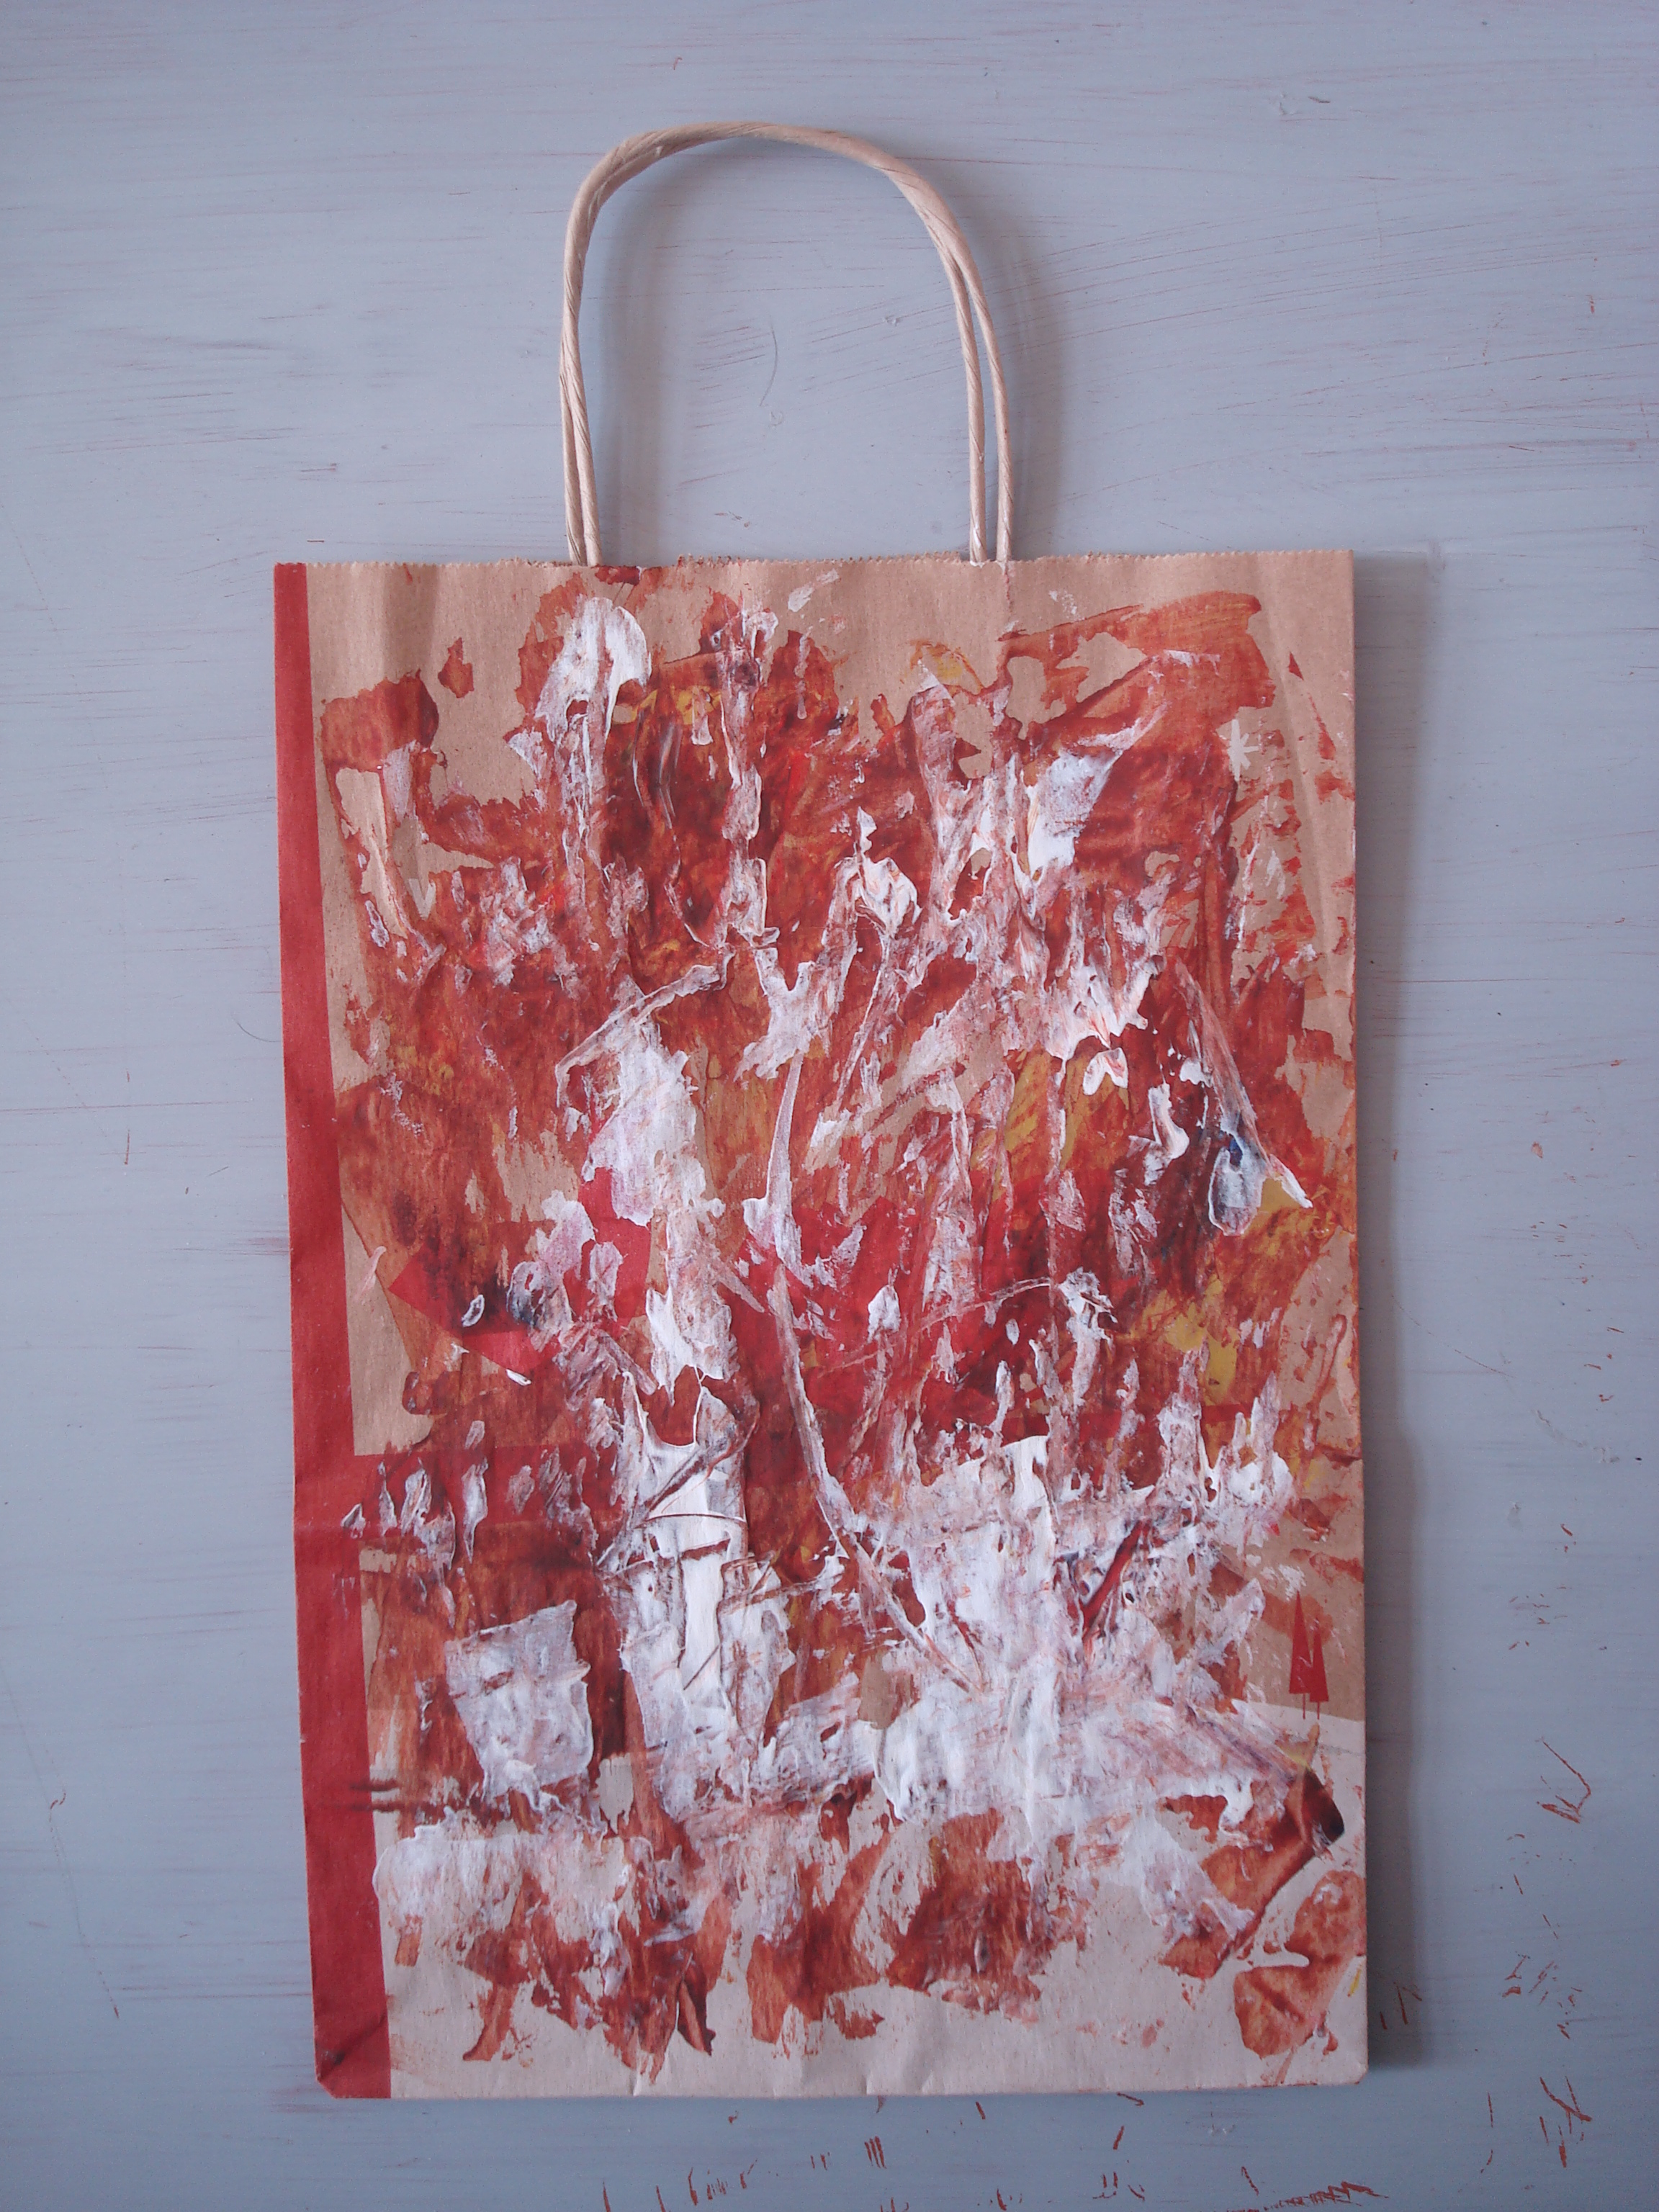
\includegraphics[width=\textwidth]{project_graphics/early_works1.jpg}
  \end{subfigure}
  \hfill
  \begin{subfigure}[b]{0.31\textwidth}
    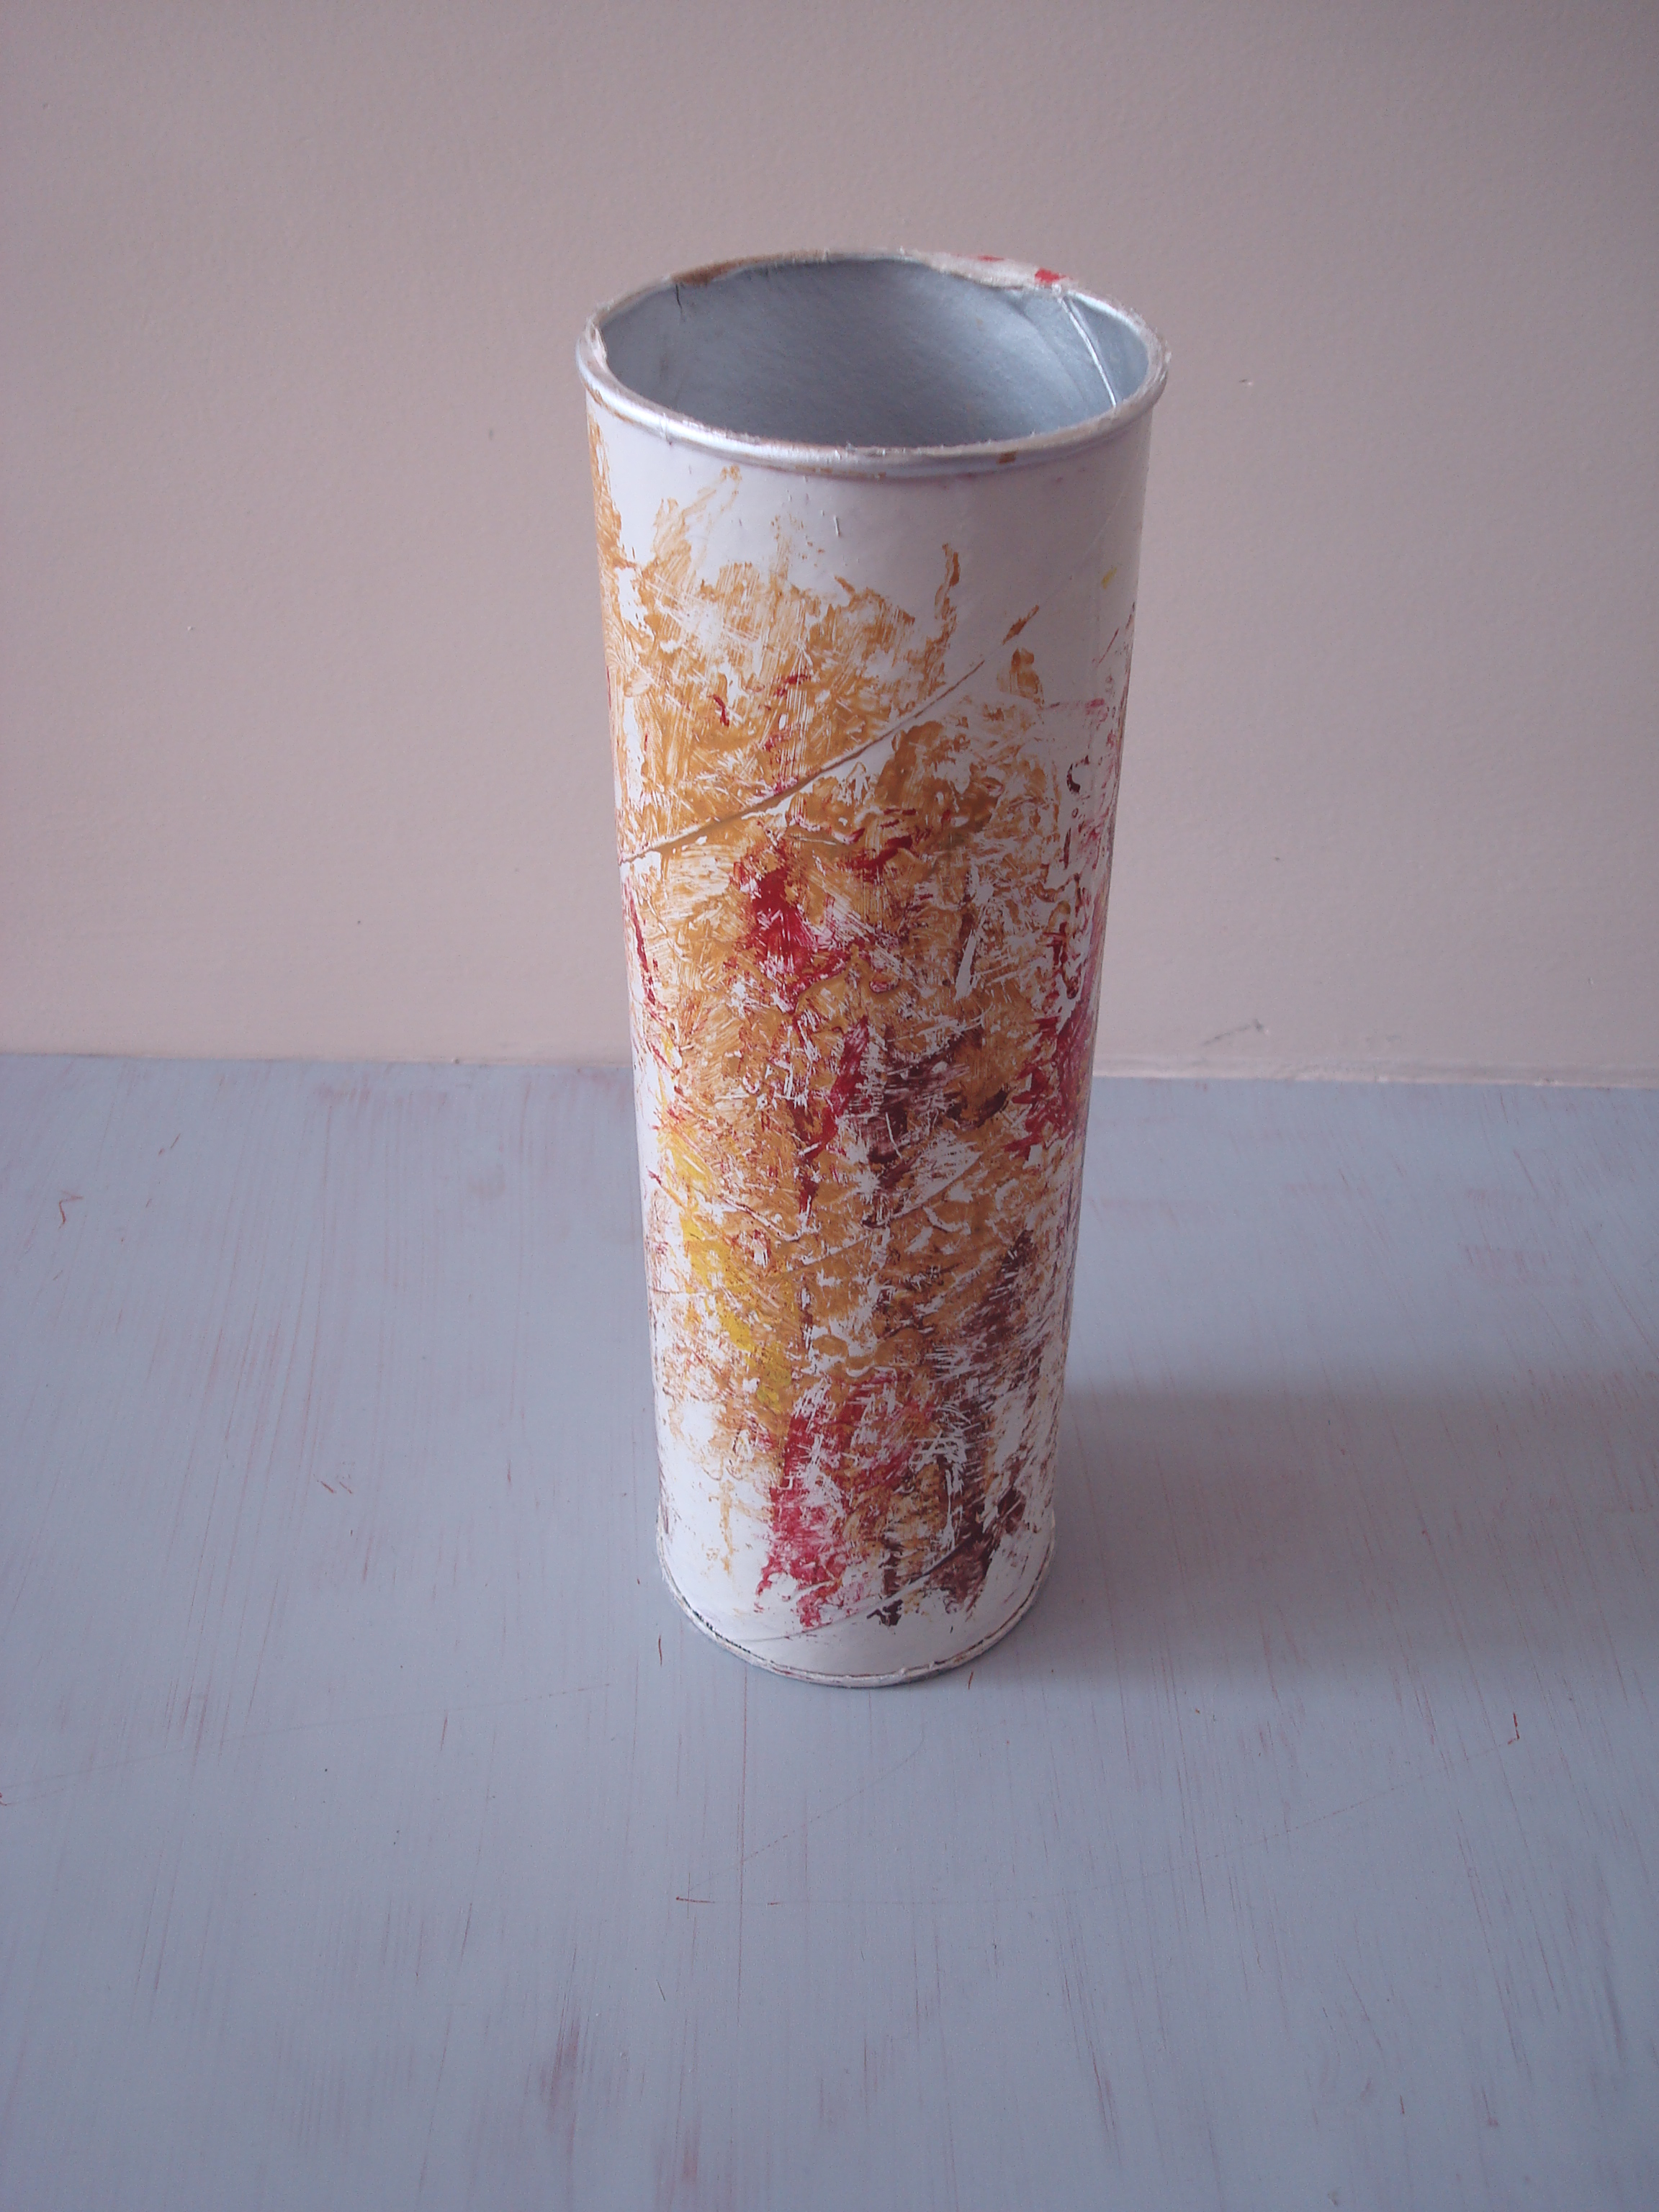
\includegraphics[width=\textwidth]{project_graphics/early_works2.jpg}
  \end{subfigure}
  \hfill
  \begin{subfigure}[b]{0.31\textwidth}
    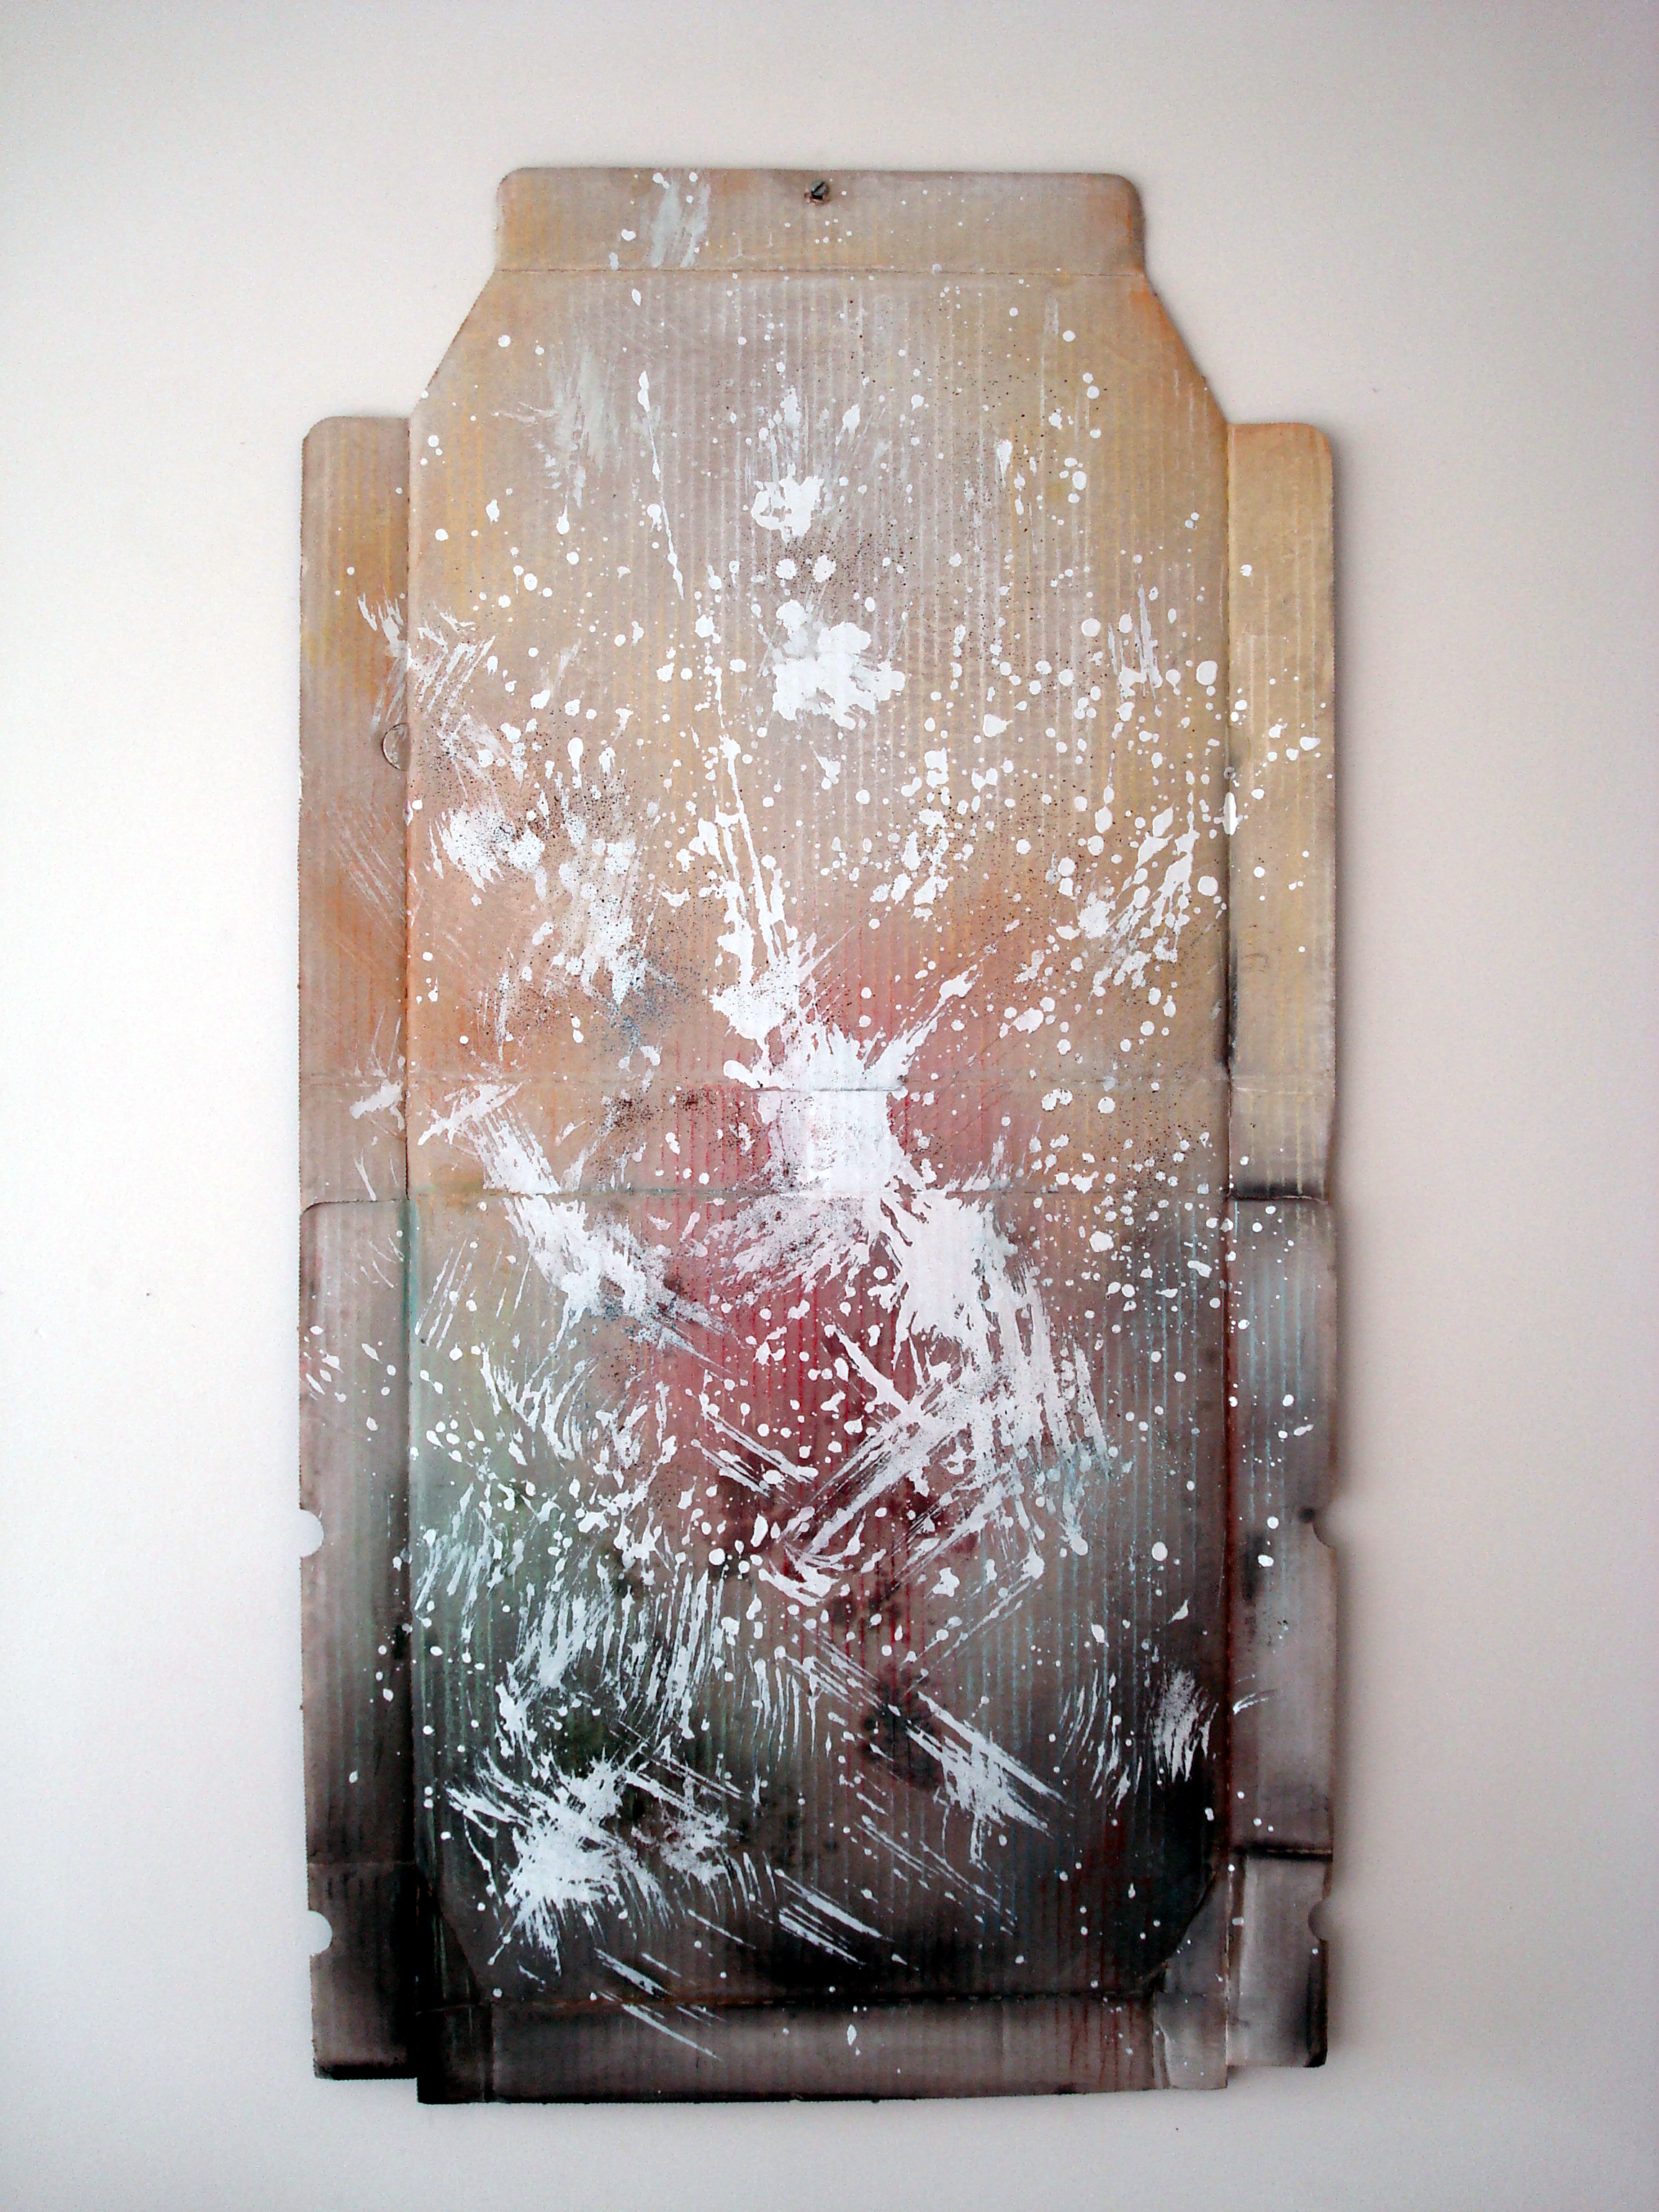
\includegraphics[width=\textwidth]{project_graphics/early_works3.jpg}
  \end{subfigure}
  \caption{Examples of early works}
  \label{fig:EarlyWorks}
\end{figure}

% TODO Free material add reference here.
My purpose in these work is to paint on different surfaces, experiment new materials. They are not flat, not blank. These surfaces bring their previous histories to the painting. Another factor is they are free and easily available. Therefore I can make many experiments on these materials. After I completed them, I showed them people around me and give them as a gift.

After turning discarded materials to different uses I began to collect them more eagerly. At the same time I also gave what I did to my friends as a birthday gift. I was experimenting with the material and at some point with the help of my mother I made my first notebook covered by Starbucks package. Papers inside of it are blank mimeograph paper which different than white paper. Particularly purpose is to move away from white paper because I feel uncomfortable when using it. It looks to me very bright. Therefore mimeograph paper is better for me. At that time it was a great victory for me. I started to carry it and use it every possible place. I show them to people and some of them supported to me giving their discard. One of them is my supervisor. He started to collect packages for me. After turning his packages to notebooks, he suggested me to go deeper in this subject and make my thesis project from them. Thereafter what I need is more discarded material.

% TODO Lars Eighner BIB'e eklenecek.

% NEW PART [collecting] 
\subsection{Collecting}
Collecting discarded objects has carried out through the efforts of mine and people around me. Lars Eighner's instructions helped me a lot when collecting objects. He writes that:

\begin{quote}
Eating safely from the Dumpsters involves three principles, using the senses and common sense to evaluate the condition of the found materials, knowing the Dumpsters of a given area and checking them regularly, and seeking always to answer the question \singlequotes{Why was this discarded?} \citep[as cited in][6]{strasser1999waste}.
\end{quote}

Does it discarded because of rotten, not fitting industrial standard or being production excess? For instance, in the documentary film of Agnés Varda, she records the potatoes that are discarded because of not fitting the industrial standards. Therefore these potatoes fall into the category of eatable.

I applied above instructions to my case and I checked discovered places regularly and seek the reason of why was it discarded. I also checked the condition of material. However I need to explore different locations to collect items. Most of them are not obvious for me. I discovered them on the flow of normal life and tasks. Similar to the methodology of Dick Jewell when searching for photos, my mode of search includes waste bins. However every object have a different story and they will be explained later.

Moreover there are other rules that define the frame of collecting act. Paper or package must be trash or will be trashed. For this project anything must not intentionally bought to use as trash. In other words first rule is to consume less and generate less trash. Lots of trash is already produced every time everywhere. Aim is to reach them.

% OWNER
\quotes{The question of who owns these discards is not trivial} \citep{zimring2012encyclopedia}. This question makes me feel uncomfortable because of thinking that stealing that someone elses' objects. Particularly I felt it when collecting leaved out papers from Bilkent Computer Laboratory. You already know that it owned by somebody else and after a while owner can take them. I solved this issue checking the leaved papers in every couples hours. If it stays there I take them. Further I encountered that If nobody takes them for a long time servants collect them.

The issue of owner becomes more complicated when owners' social status considered. Zubiaurre mentions that no body cares her student scavenged through people’s trash in a poor neighborhood \citep[as cited in][]{pricano2011trashtalk}. On the contrary when the same student went to Beverly Hills home of the many actors and celebrities in California to scavenge nearly the police were called.

% CONTRIBUTIONS OF PEOPLE
As mentioned previously many people contributed to the project by collecting. Whenever I meet my friends I ask them to save their discard for the project. The importance of collaboration with them can be understood the term "citizen science" which is \quotes{defined as scientific research performed in part or in whole by volunteers who are not professional scientists} \citep{robson2012using}. I need to note that this is not a scientific project but the notion belongs there. The value of it lies in the collective intelligence of the contributors. In the scope of this thesis the term can be interpreted as people bring their own creativity and interpretation to the project by collecting the items that they reach and select. When the number of contributors are increased the diversity of the collected material will be increased and this will echoed in the notebooks. 

It can be viewed as a co-authored work. Because many people helped me to collect the papers and also many people leave their trail to the paper and also they bring meaning to the them. After production of papers I also want them to continue as co-authored process. In other words many people will be part of this project. As people see different things on objects and bring them to me. the variety of things is increased in time. Because people sad me that \quotes{I thought that you can use it. Do you collect also these?}. They bring their unique approach. 

They provide me the materials to transform it. They select the items and find them. They bring their approach and selection. They are part of the selection of the materials. They started to engage with the work. People bring the material also wonder the result of it. Further people see me when collecting objects and transporting them wonders their purpose. 

The purpose is here not only to transform objects but also change the perceptions of trash. Asking people to collect things and inform them started to shift in peoples mind.

Collected items reflect my and contributors' consumption practices. People as mentioned previously consumption patterns can be tracked from their leftover. From logos of companies onto the packages reveal people's choices and give clues about their social status.

% What type of activities generates waste.
Beyond social status it reveals activities that generate such a waste.It can be also extracted that most of the trashed papers are thrown away from feeding activity. On the other hand vastness of some types of disposables reveal the dark side of the enterprises such as Starbucks and Burger King. Few people thought that after seeing the project I only collected Starbucks packets. There is no such a limitation but as a result of my habitat the number of them suppress the others.

%[disposable paper, packaging]
Collected items are mainly disposables ones. Most of them are paper or made from paper. The word paper comes from papyrus, the plant that was first used for writing in ancient Egypt long before the making of paper in China. In modern times all types and qualities of paper such as newspaper paper, print paper, and carton used for boxes pass through the same basic method of manufacture \citep{trafford2012paper}. It is fundamental medium for writing, reading, education, communication, information storage and many others. Its role in the development of human civilization can not be neglected. (Paper in several forms is consumed on a daily basis \citep{trafford2012paper}.) Wide range of use from packing to newspaper makes it indispensable product for people. On the other hand for artist it offers great diversity in order to make compositions as can be seen in the works of collage. Further it is easy to find and collect them. Even if it is thrown out, still appropriate for painting and writing.

Since paper is both biodegradable and a renewable resource, it is preferred by some of corporations for their products to show their respect to the nature. The motivation why they use can be seen their notes printed on the papers (Figure \ref{fig:NoteOnPackage}).

\begin{figure}[h!]
  \centering
  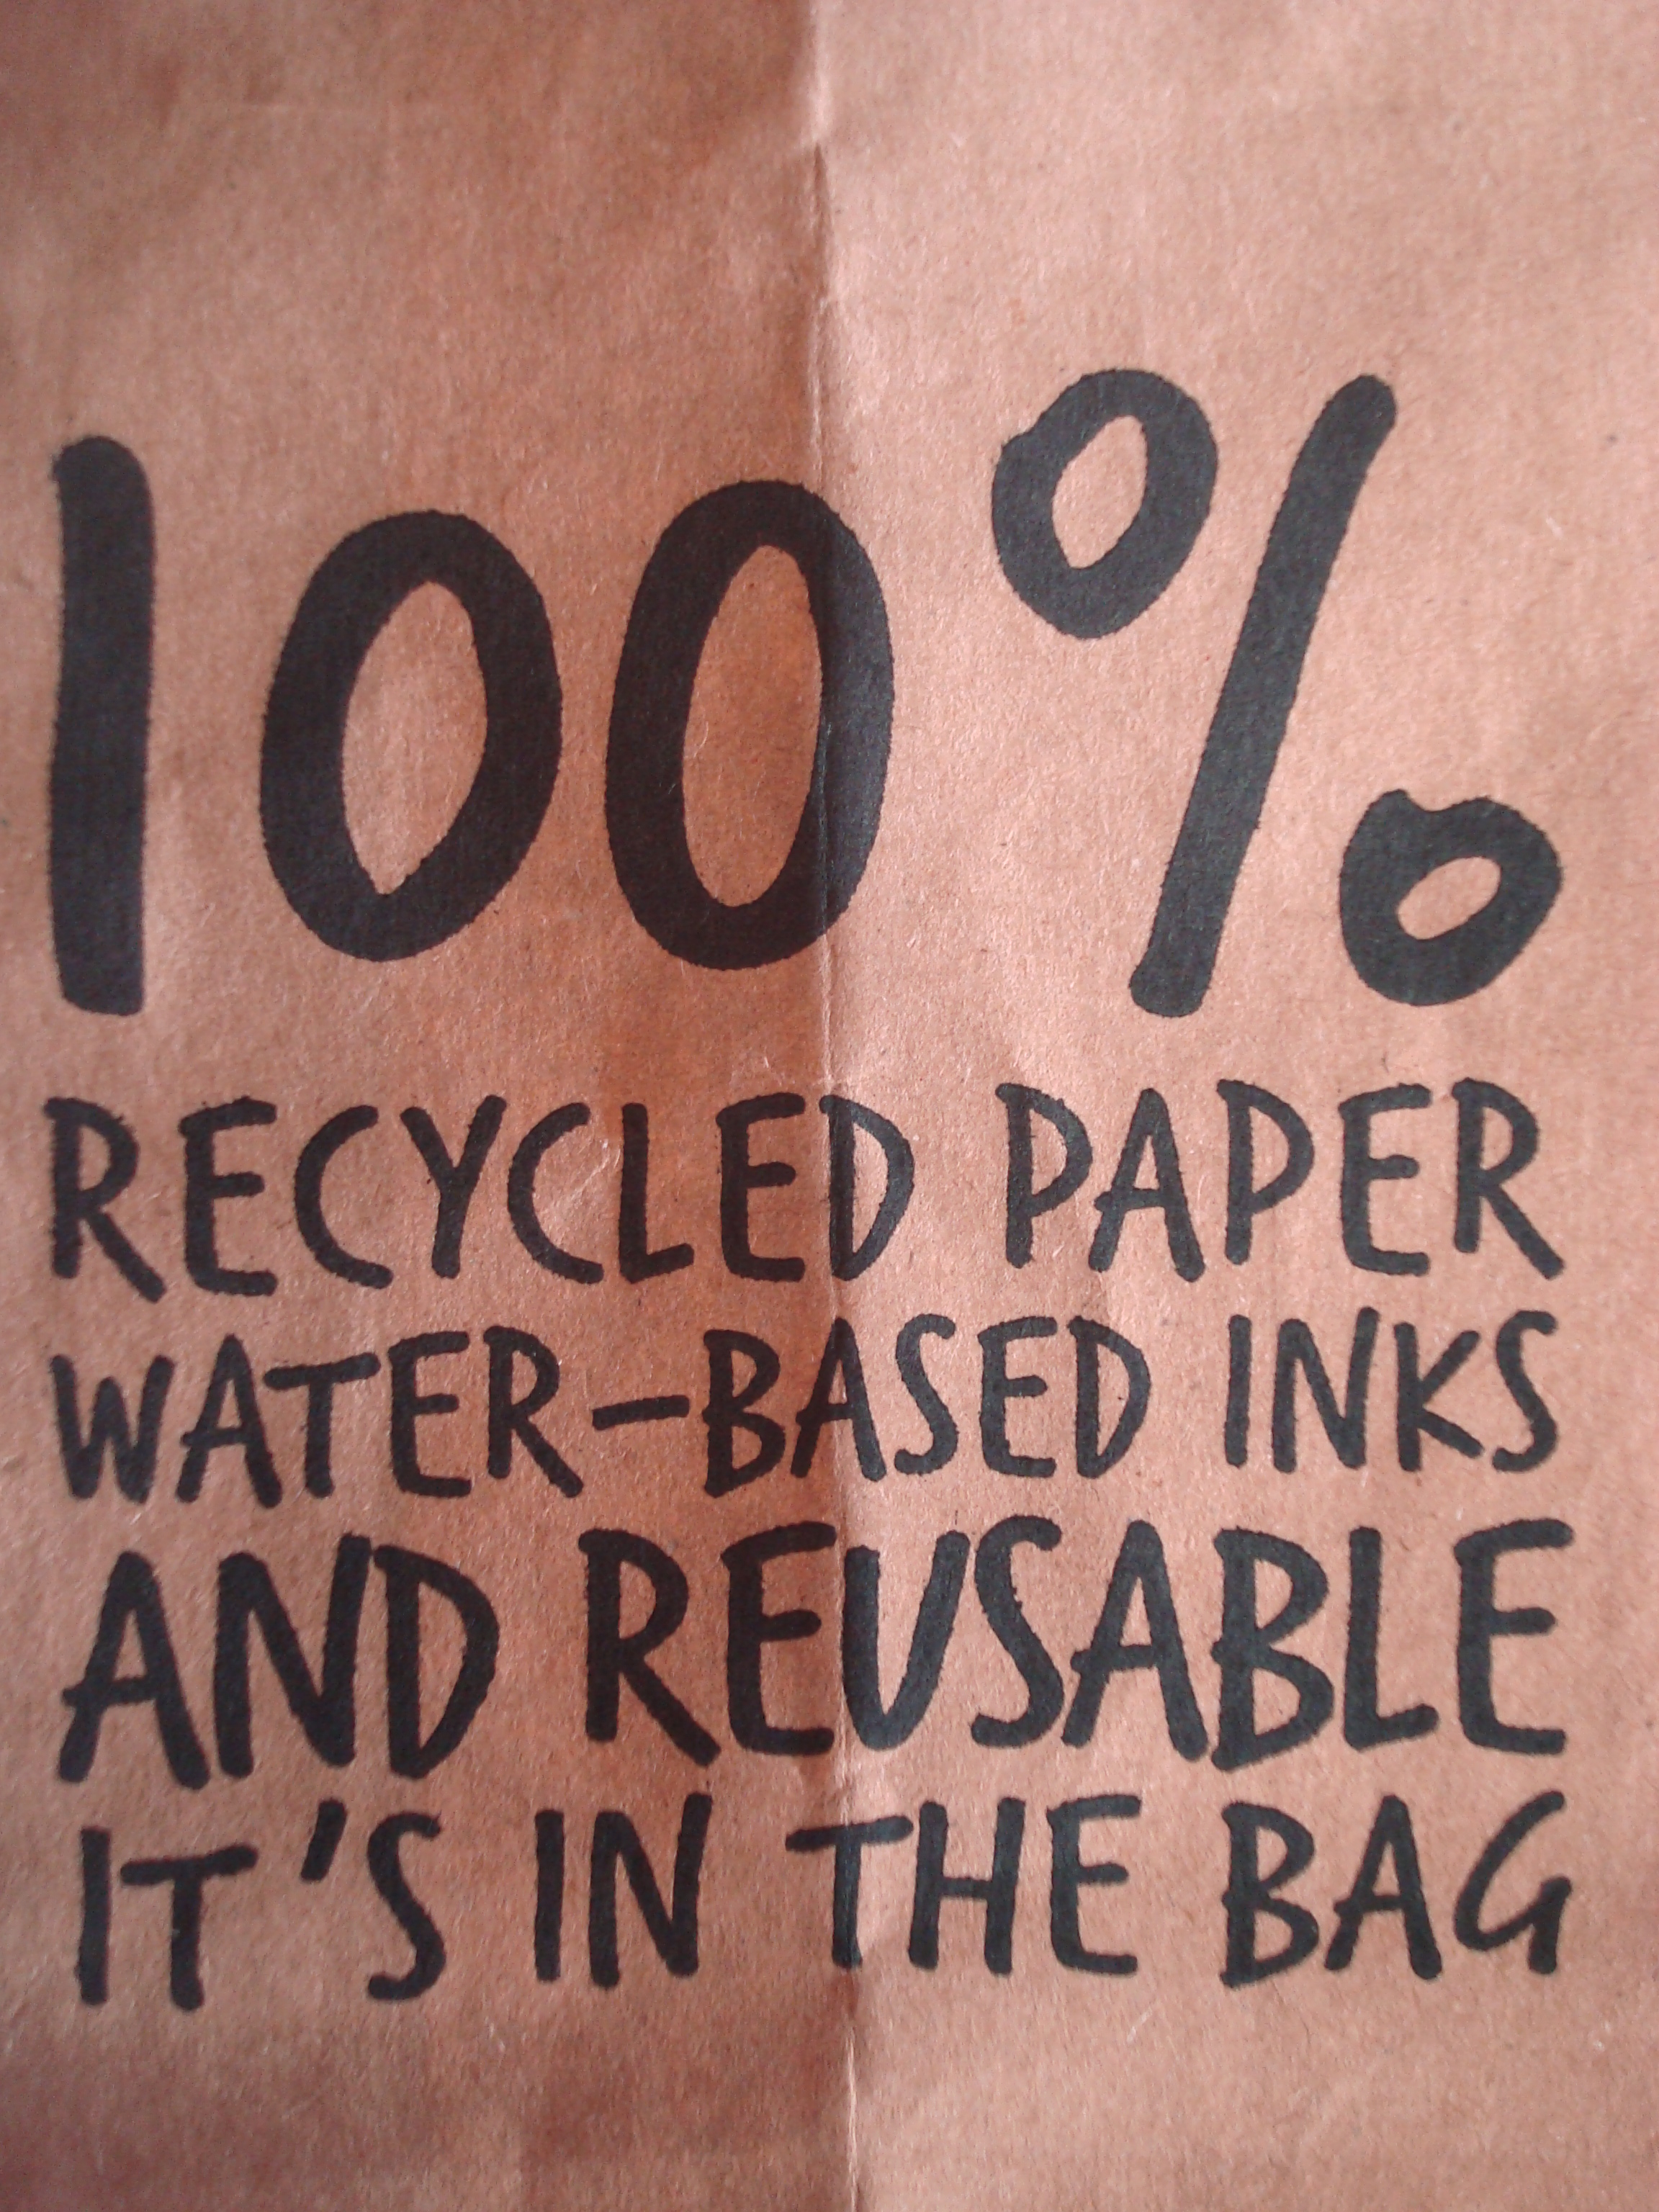
\includegraphics[height=6cm]{project_graphics/recycled_note.jpg}
  \caption{Recycling notice on the package}
  \label{fig:NoteOnPackage}
\end{figure}

The reason of collecting papers based on my interest on painting and writing. This medium offers me great possibilities that I cannot consume yet. This project is one of them.

% TODO see figure appendix.
Collected items are stored in my room for a long time. Most of them are not belong to me. Here the detailed information of the collected materials including the place where it is collected and their previous usage are listed.

\textbf{Burger King packages} are collected from the office where I work. At launch time, some of the colleagues order their meal from Burger King which is a global chain of fast food restaurant. Meals are delivered to the office with paper packages. The package of the meal is collected and used as a cover of notebooks. 

Inside the bag one paper package is used for French fries which is oily and paper is very good to absorb oil. Some people think that it is disgusting to use it for other purposes because of oil onto it. But immediately I replied them \quotes{you just eat that oily fires so what is wrong with it?} At the same time what \cite[5]{strasser1999waste} said comes to my mind; \quotes{Nothing is inherently trash}. She refers to resolution on dirt of \cite[36]{douglas2003purity}:
\begin{quote}
Shoes are not dirty in themselves, but it is dirty to place them on the dining table; food is not dirty in itself but it is dirty to leave cooking utensils in the bedroom, or food bespattered on clothing; similarly bathroom equipment in the drawing room; clothing lying on chairs; out-door things in-doors; upstairs things downstairs; under-clothing appearing where over-clothing should be and so on.
\end{quote}

This simply explains that our perceptions to the objects are relative and change in their usage context.

% TODO relocate
%Trash is something that is out of sight, out of mind. Paid little attention to them and only catches attention when it is in wrong place. It is an unexpected object for people. Therefore transformation of it can create powerful and surprising effect onto the people. 

%\paraphrase{Thompson comments that we only notice rubbish when it is in the wrong place, and highlights the embarrassment and anxiety that mis-placed rubbish, or rubbish which has found its way in to the wrong place can cause ‘Something which has been discarded, but never threatens to intrude, does not worry us at all.’ (1979: 92) but rubbish in the wrong place is ‘emphatically visible and extremely embarrassing’ (1972: 92). Rubbish objects are things that are no longer used or loved or cared for and often no longer seen. Rubbish objects linger on the periphery of our lives, in the back of the drawer, bottom of the wardrobe or cupboard, corner of the garage or garden shed gathering dust. (Summary From Liz Parsons.)} 

\textbf{Starbucks packages} are collected from my supervisor, office where I work and my friend. Particularly my friend saved and collected them from her friends. Few of them collected from waste bins. They are used as a cover of notebooks. There are different types of packets from this category. As claimed by the company all of them are build from recycled ---precisely downcycled--- paper. There is also one category of object that is not paper. It is package of coffee beans. It is airtight and waterproof. It is very solid and strong. It has well graphic designs with different color and illustration.

\textbf{Modshifters papers} are used to cover the dinner table. Beginning of the table there is a big roll of paper to cover the table. At the end of the day used parts are cut out and thrown away. One of my visit I stayed there at a late time and catch the waiter when collecting the used papers and preparing tables to the next customer. I asked kindly him to give me these papers and he accepted. They are used as a cover of notebooks. All of them contains track of people who sit down there. I do not know any of them and I am not sure that the paper that they are laid down on their dinner turned to such a thing.

\textbf{Varuna Gezgin papers} are the pages of obsolete dinner menu. When leaving there I showed my notebooks and asked to the cashier that I could able to present them at Varuna Gezgin. He immediately mentioned their vast amount of unused papers and gave me some of them that I can able to carry with me. This was a very strange experience for me because I did not expect such a thing. These paper are used inside of the notebooks as a page.

% I'm collecting the paper that are under the plates. When we are leaving this place, I ask the cashier at the desk that \quotes{I am making small notebooks and is it possible to exhibit there?} I asked that is it possible to give them to people. Firstly he asked me that did I sell them or not but I said \quotes{no they are free and part of my thesis project.} After that he offered me to give e are a lot of unused papers. I can give you. they are not used and waiting to be recycling. I took some of the papers, and that papers are part the sheets of these papers.

\textbf{The banner} is carried at graduation ceremony of Middle East Technical University in 2011 by the new Computer Engineering graduates. In Middle East Technical University there is a tradition that in graduation ceremony new grads walk through in the stadium and greet to the tribunes. With this event they carry some banners to express their feelings and point out the issues of the country in an ironic and humorous way. This one of them. At that time there are serious debates about freedom on the web. Most of the website are banned from the decision to the courts and they were not accessible. The slogan (Access to this banner is blocked by a court decision) decided by the new grads and before the ceremony I printed out the slogan to carried out as many people as it can and easy to readable from the people who seat at the tribunes.After the ceremony I could not throw away this banner. I do not know what to do it. It is a very big roll of paper to save but I could not throw away. I think that I will figure out later. Maybe I can use it as a draft paper. However is it worth to cut out this all long banner? Moreover to strengthen the banner we tape it from its boundaries. In other words some of the areas can not appropriate for writing. When I decided to my thesis subject I remembered to this banner. It stands in a corner in a dusty way. Now it is time to use it. It waited very log time and it is time to revive. I cut out them to the smaller pieces to use them as pages of notebooks. All pages have unique patterns. They contain parts of letters. Most of the time it is not recognizable belongs to which letter. These papers offers unique writing experience to the writer because of the patterns of letters and residue of tapes.

By the way currently in Turkey the problem of banning web-sites continues. Event it can said that people do not surprises when a website is blocked by the courts. In other words still the slogan preserves its significance and through this project people will remember these days.

\begin{figure}[h!]
  \centering
  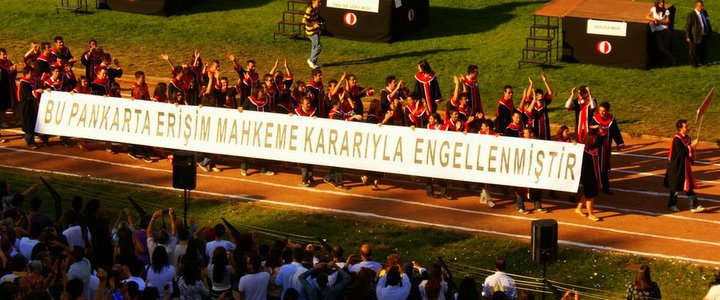
\includegraphics[width=1\textwidth]{project_graphics/banner1.jpg}
  \caption{The banner carried by new grads, 2011}
  \label{fig:Banner_1}
\end{figure}

\textbf{Order slips} are collected from bank office located at Technopolis of Middle East Technical University. They are used to record the order of customers. I realized that back of them are empty and appropriate for writing. Further there many others are waiting on the bin. After this experiment I really convinced that I am really looking for trash everywhere every time. The act of collecting spread through the every moment of life. 

\textbf{A4 photocopy papers} are collected from Bilkent Computer Laboratory. In every lab there is a one printer. However when someone wants to print computers suggest firstly printer on the room 307. This result in many confusions and extra prints. I explored this place during my thesis research. I went there to print out draft of my thesis. I encountered that many papers are leaved on the tables.  The reason of why they are leaved behind is not obvious but technical errors, printing wrong versions and extra copies can be easily guessed after a little observation. Nobody cares others print out. Papers are mostly composed of lecture notes. I collected many papers from there and they are used as a page of notebooks. I do not know owner of them and possibly users of notebooks so. However it will increase our realization of what other students in this university are dealing with.

Similar type of papers are also taken from my friend. They are composed of his lecture notes. He donated them to the project.

Collected items are not limited with these but for the others there are no special memory. Tea bags, collected packages from the streets are some of them.

Most of the materials that I collect are mass produced items. Generally their usage fall into the two category; education and food industry. They are found on public places. They are not personal objects like in the work of Tracey Emin's \quotes{My Bed} even if it can be claimed that the collected papers from the laboratory contains personal travel tickets. Identity of owner are not certain.

% Elimde bazılarının fotoğrafları (kayıtları) var bazılarının ise yok.

% burdaki dikkate alinan sey satilan bir sey olmadigdi. Kütuphanede ise aslinda bunun bir reklam anlami tasiyip tasimayagi idi. Bilkent labindakiler ise bunukomsenin almayacagi dokunmayacagi yonundeydi. E napalim artik. Insanlarla konustukca farkli seyler dusunuyorum.

% ozellikle resterantlardan bunkari tplarken, genekde garsonlar hemen almaya calisiyorlardi. Ben topladigimi soylerken bu zman yenisini getirmeyi teklif ediyorardi. Bu benim onceden bahsettigimaz tuketme kurali ile celismekteydi ve ben bunu reddediyordum.





% NEW PART [transforming]
\subsection{Transformation}
At one side while paper is being collected, on the other side I started to make experiments with the material. I questioned what else can be made with these collected materials and tried to cover (wrap out) objects and plants in the public. However these do not give the result what I want. People cannot interact with these and possibly they will turn to trash again. For that reason the first approach which is making notebooks are more appropriate to accomplish the purpose.

\begin{figure}
  \begin{subfigure}[b]{0.48\textwidth}
    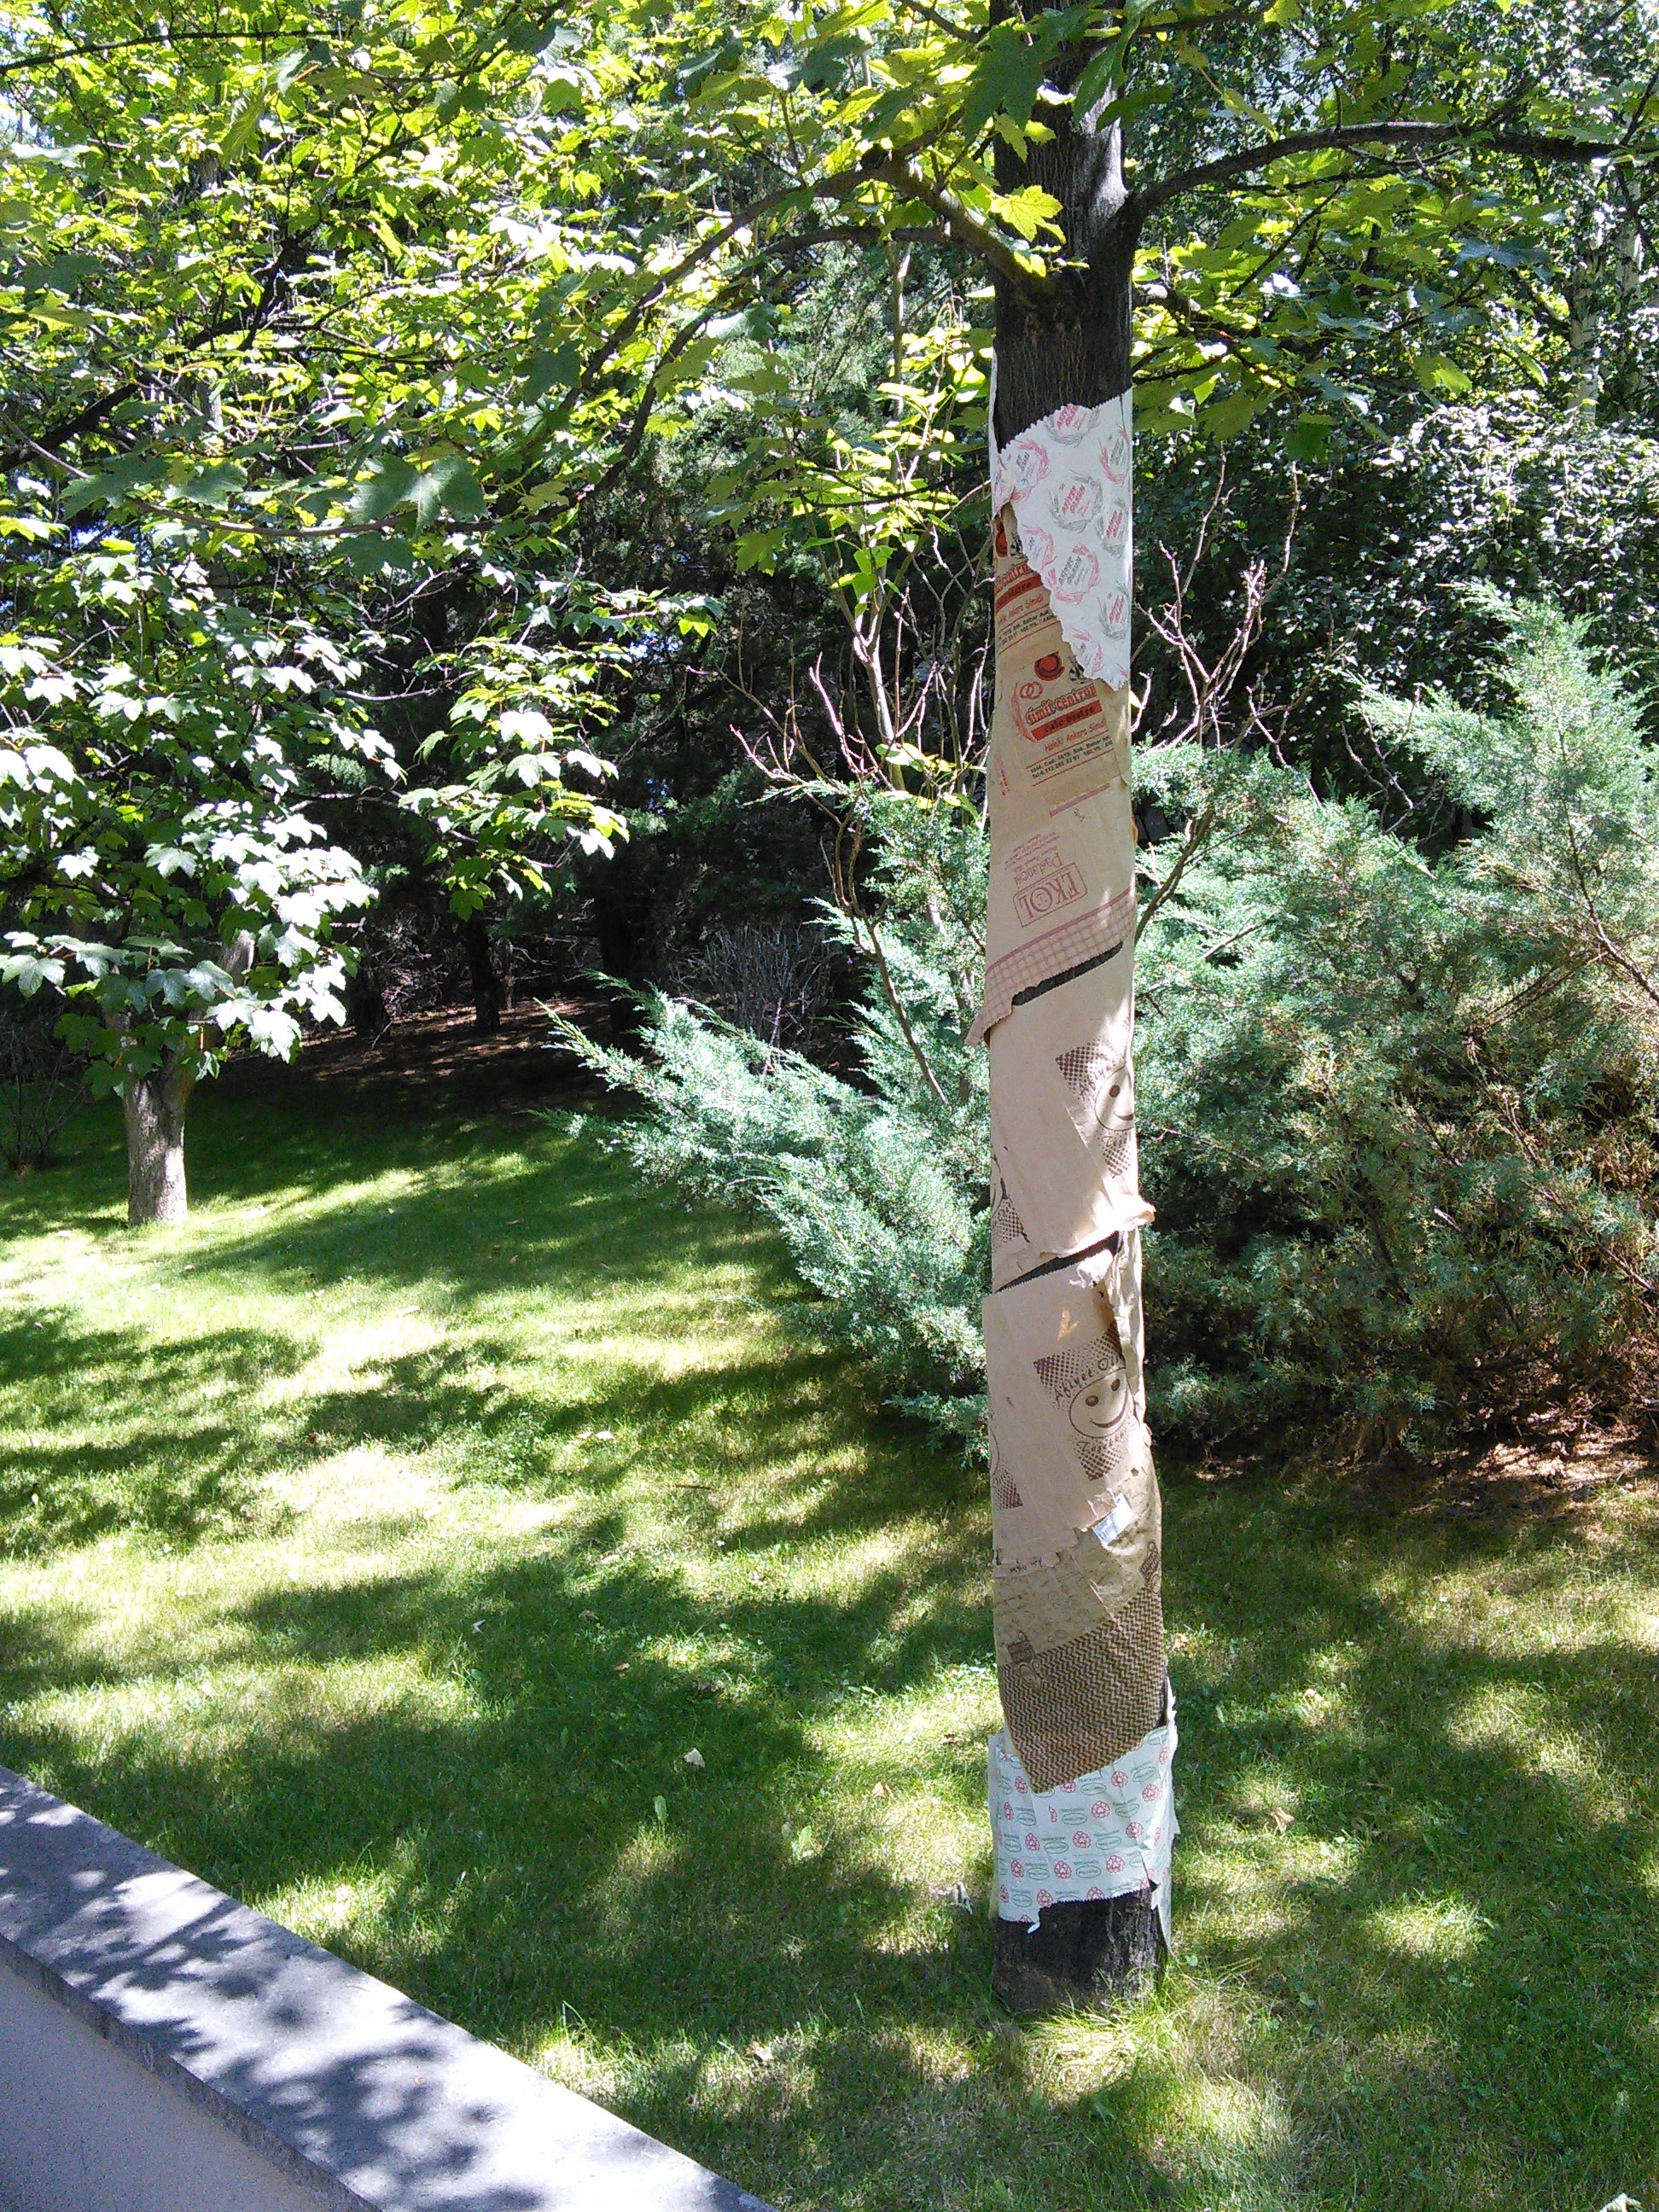
\includegraphics[width=\textwidth]{project_graphics/tree_experiment1.jpg}
  \end{subfigure}
  \hfill
  \begin{subfigure}[b]{0.48\textwidth}
    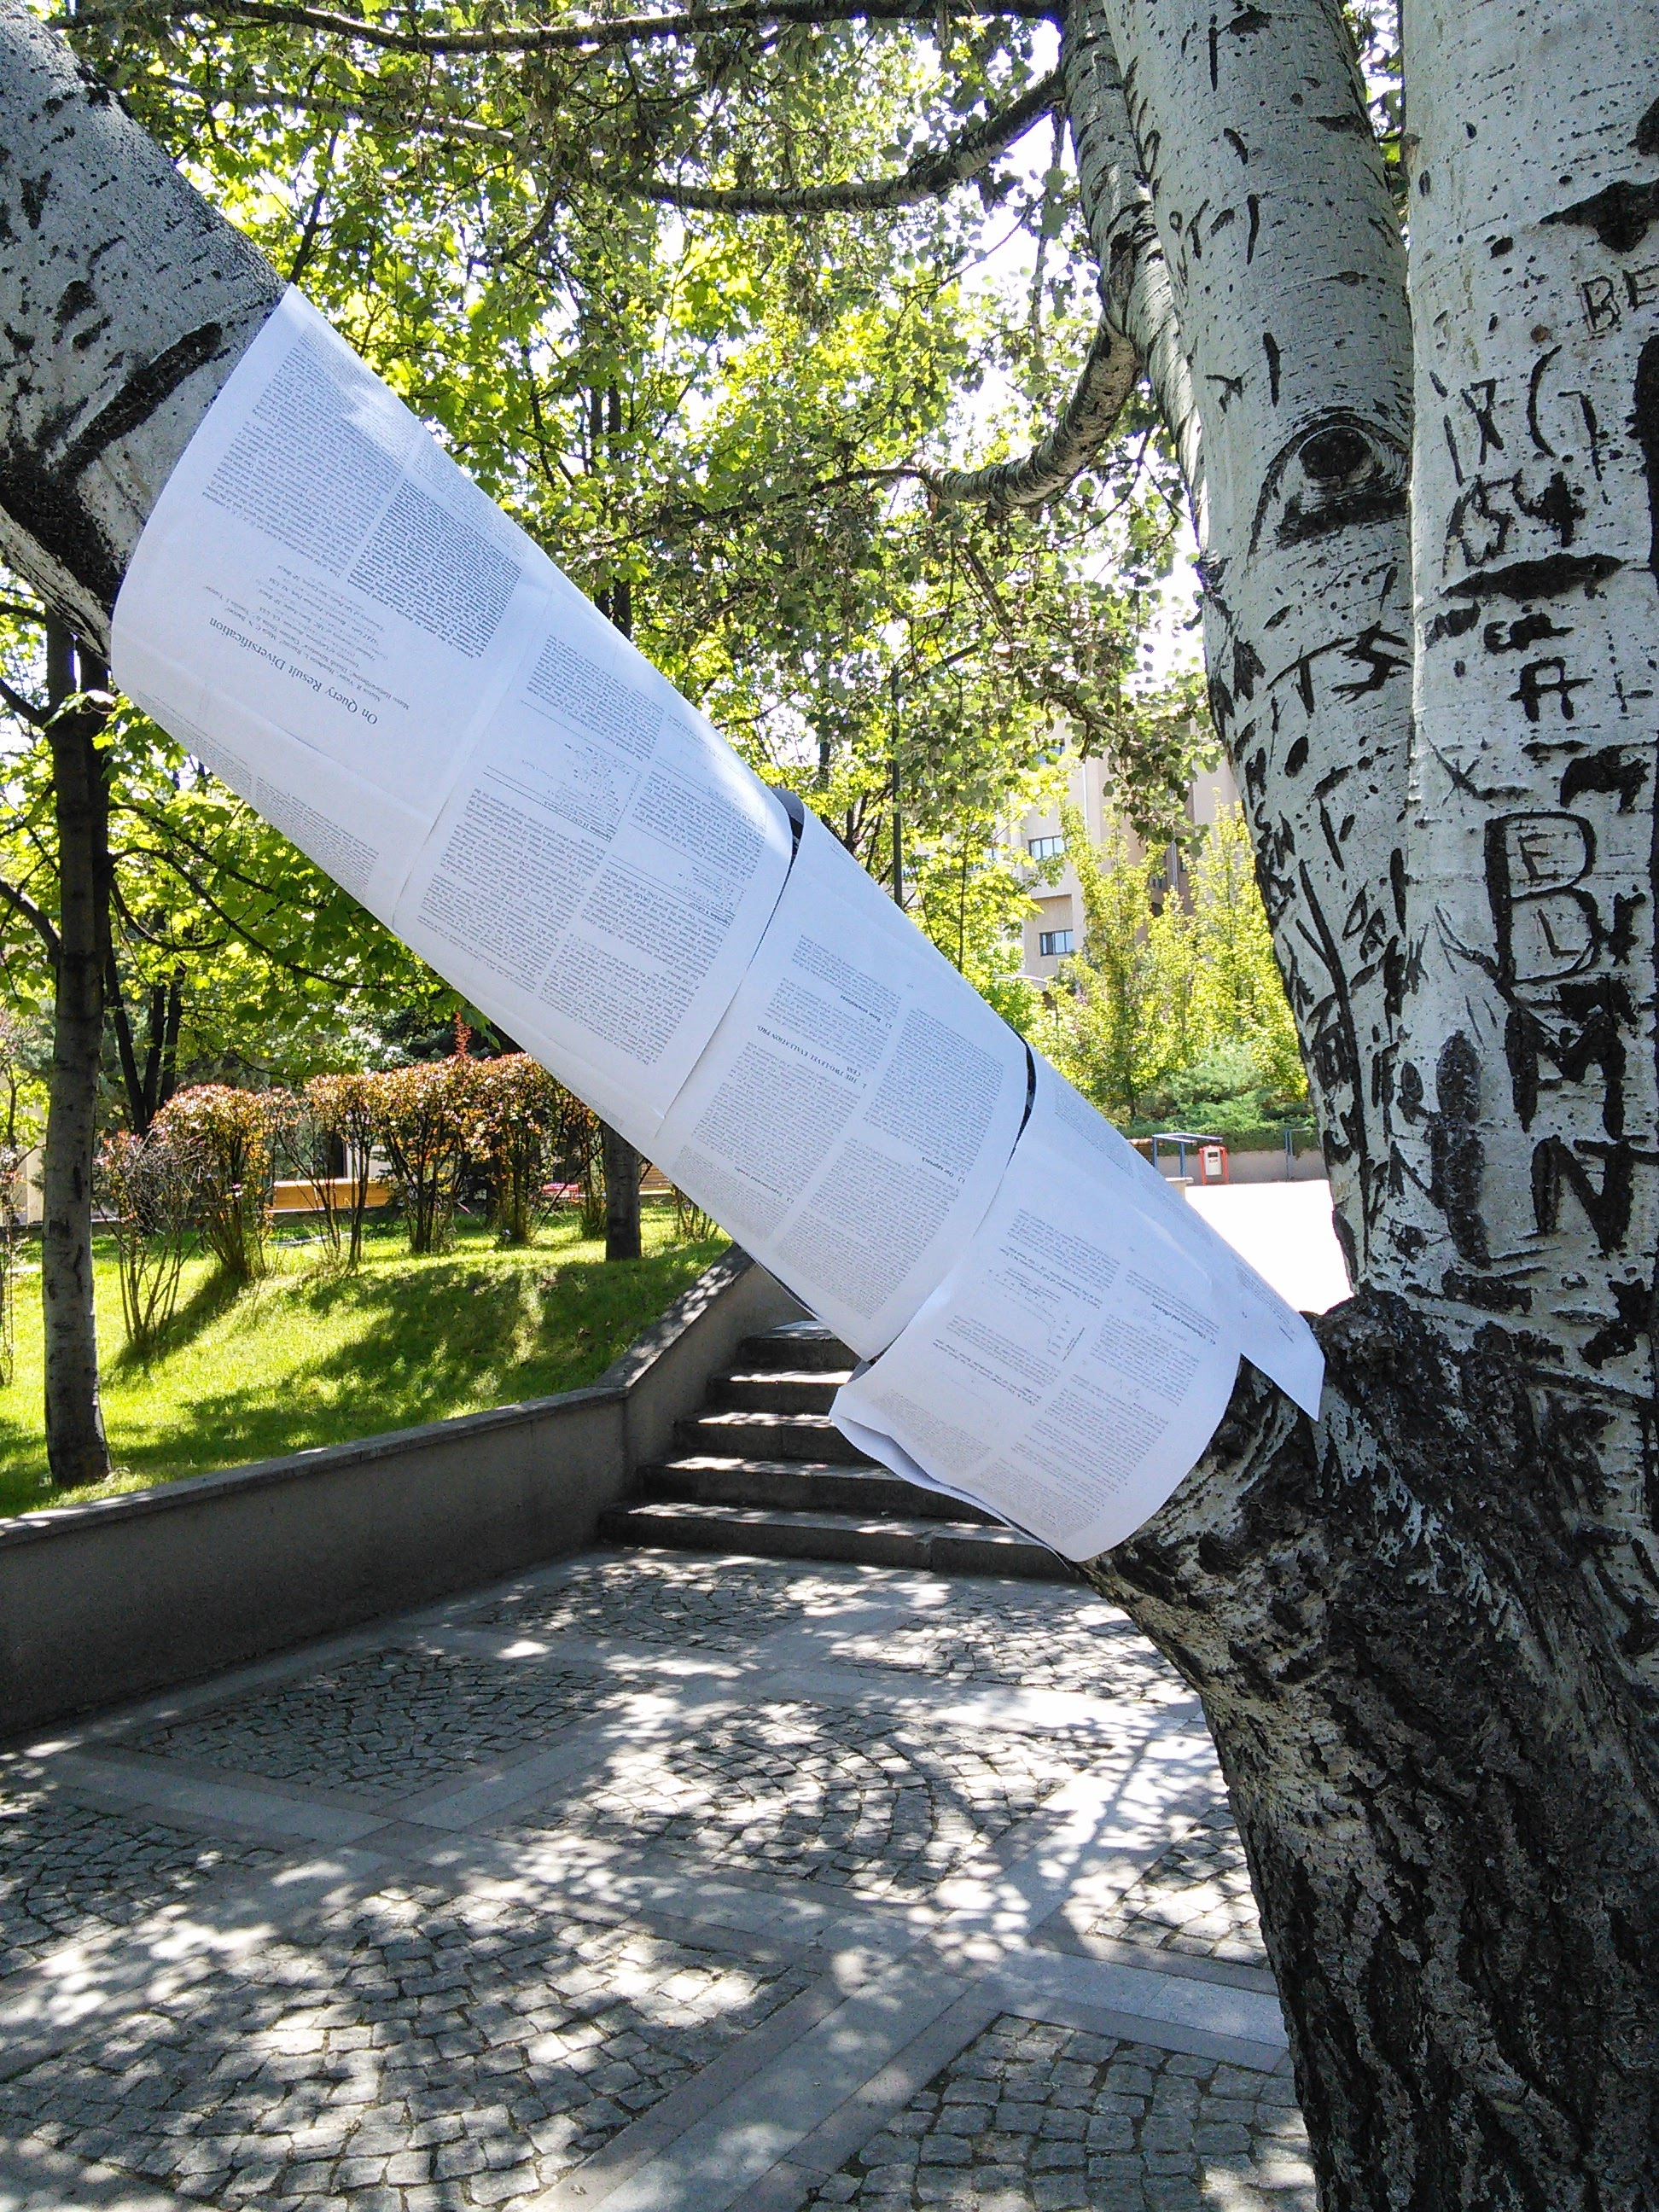
\includegraphics[width=\textwidth]{project_graphics/tree_experiment2.jpg}
  \end{subfigure}
  \caption{Experiments with collected papers}
  \label{fig:ExperimentWithPaper}
\end{figure}

% [notebooks]
There are two main parts of notebooks; cover and pages. Papers that are mostly blank(empty) are used inside of the notebooks for writing. Others that are solid and colorful are used as a cover for notebooks. Mixing (juxtaposing) materials is main method in the production process. I combine different papers and packages. I try to generate every possible combination. The purpose is to create as many alternatives as I can because trash is ignored and people do not give it new alternatives. Therefore these notebooks provide many alternatives to show that otherwise is possible. 

Technically papers combined together by sewing and gluing. I learned sewing techniques from my mother and the gluing part is trivial. For this project I need to produce dozens of notebooks. However through time I started to produce them more rapid by improving my technique. One of the struggles that I faced is to punch holes with needle. At this process I cracked a needle. Later I discovered that with the help of pushpin punching the holes becomes more easy. After punching holes I just followed the holes with needle. I used nylon yarn which is solid and thin. Being thin is important it must fit into the opened holes. After sewing them I fixed the yarn with hole by gluing to make it more solid.

I followed the methods of Dada poem to mix the papers used inside of the notebooks. I changed their order and direction. 
\cite{tzara1977seven}, gave the following instructions on how \quotes{[t]o make a Dadaist Poem}:

\begin{quote}
Take a newspaper. Take some scissors. Choose from this paper an article the length you want to make your poem. Cut out the article. Next carefully cut out each of the words that make up this article and put them all in a bag. Shake gently. Next take out each cutting one after the other. Copy conscientiously in the order in which they left the bag. The poem will resemble you. And there you are ---an infinitely original author of charming sensibility, even though unappreciated by the vulgar herd.
\end{quote}

% TODO starbucks defterlerinin hep yapıştırılmış olmasını da eklemek gerekli.

% TODO muhakkak tekrar kontrol etmek gerekli.
Size of the paper used inside of the notebooks are mostly equals to the size of an A4 sheet. Usage of papers differs among the notebooks. Especially for the papers taken from Varuna Gezgin written part is folded inward by hiding it. However for the ones collected from Bilkent Computer Laboratory written side of it leaved open. Their content comes from various students whose departments are also various. In other words offers great diversity and they are mixed to allow different interpretations. Further it provides what students from other departments works on. What other students work on can be understand from these.

There are different dimensions of notebooks. Most of them are half of A4 or quarter of it.

% TODO Dimensions of notebooks. most of them half of A4 or quarte of it. böyle bir fotoğraf eklenmeli. farklı boyutlarda farklı şekillerde ve renklerde.

% TODO defterin yakından fotoğrafları

% TODO defter dikme yönteminin fotoğrafı

The tools used in the making of notebooks are as follows; needle, sewing thread, scissors, utility knife, pushpin, silicone, caulking guns.

While transforming collected materials my method can be explained with the term upcycling mentioned at the end of the Chapter 1. Further I tried to use objects already at hand. In other words I followed the bricolage technique. However I have to do buy some tools for my work. Therefore it is hard to consider it as bricolage but my intention is to follow it.

Moreover I have reviewed other notebook projects. Notable ones are The Sketchbook Project and myDetour from Moleskine. In these projects anyone who bought the notebooks from them can participate and send their notebooks filled with illustrations and paintings. These projects can be seen as crowd-sourced library. Further the pages of the notebooks are available at online. After checking sketches in these notebooks, the diversity of them surprised me a lot. It forced me think that the transformation process is not limited with the production of notebooks from trash. After notebooks are given to the people, their transformation will continue. Therefore I think the process of transformation is a continuous act.

% The purpose is here to increase the diversity.

% Çok basit bir şekilde çöp olarak görülen bir şeyi başka bir şey olarak görmek keyifli bir şey benim için. zaten dönüştürmek kullanmak için topluyorum.

% Dönüştürme sebepleri. Neden sadece toplamakla yetinmiyorum. Yeni kompozisyonlar oluşturmak istiyorum. Farklı karşımlar elde etmek istiyorum. Bir tür şaşırtmak durumu... Beklenmeyeni yapmak... En olmadık malzeme çöple çalışmak bu yüzden önemli benim için.

% [Artistic tactics] Here I followed some tactics to accomplish my purposes. Easy to carry while traveling. Small notebooks. Placing them to their routes.

% bi de ben bunu insanlara vermek istiyordum o yüzden defter iyi bir şey. ve bu benim aslında bir taktiğim arkadaş. defter insanın yanında taşıdığı kullandığı bir şey. sadece galeri de olmayan başka alanlara da sızan bir şey olması önemli. 





% NEW PART
\subsection{Demonstration}
After producing notebooks the most important point is to present and reach to people. Main question is how to give them to people. Starting point is to stack the notebooks onto the each other, and there are other ideas like putting them inside a waste bin to re-do the action of throwing away. After ward somehow they should understand that these notebooks can be taken. I set up models and tried some installations of them.

\begin{figure}
  \begin{subfigure}[b]{0.31\textwidth}
    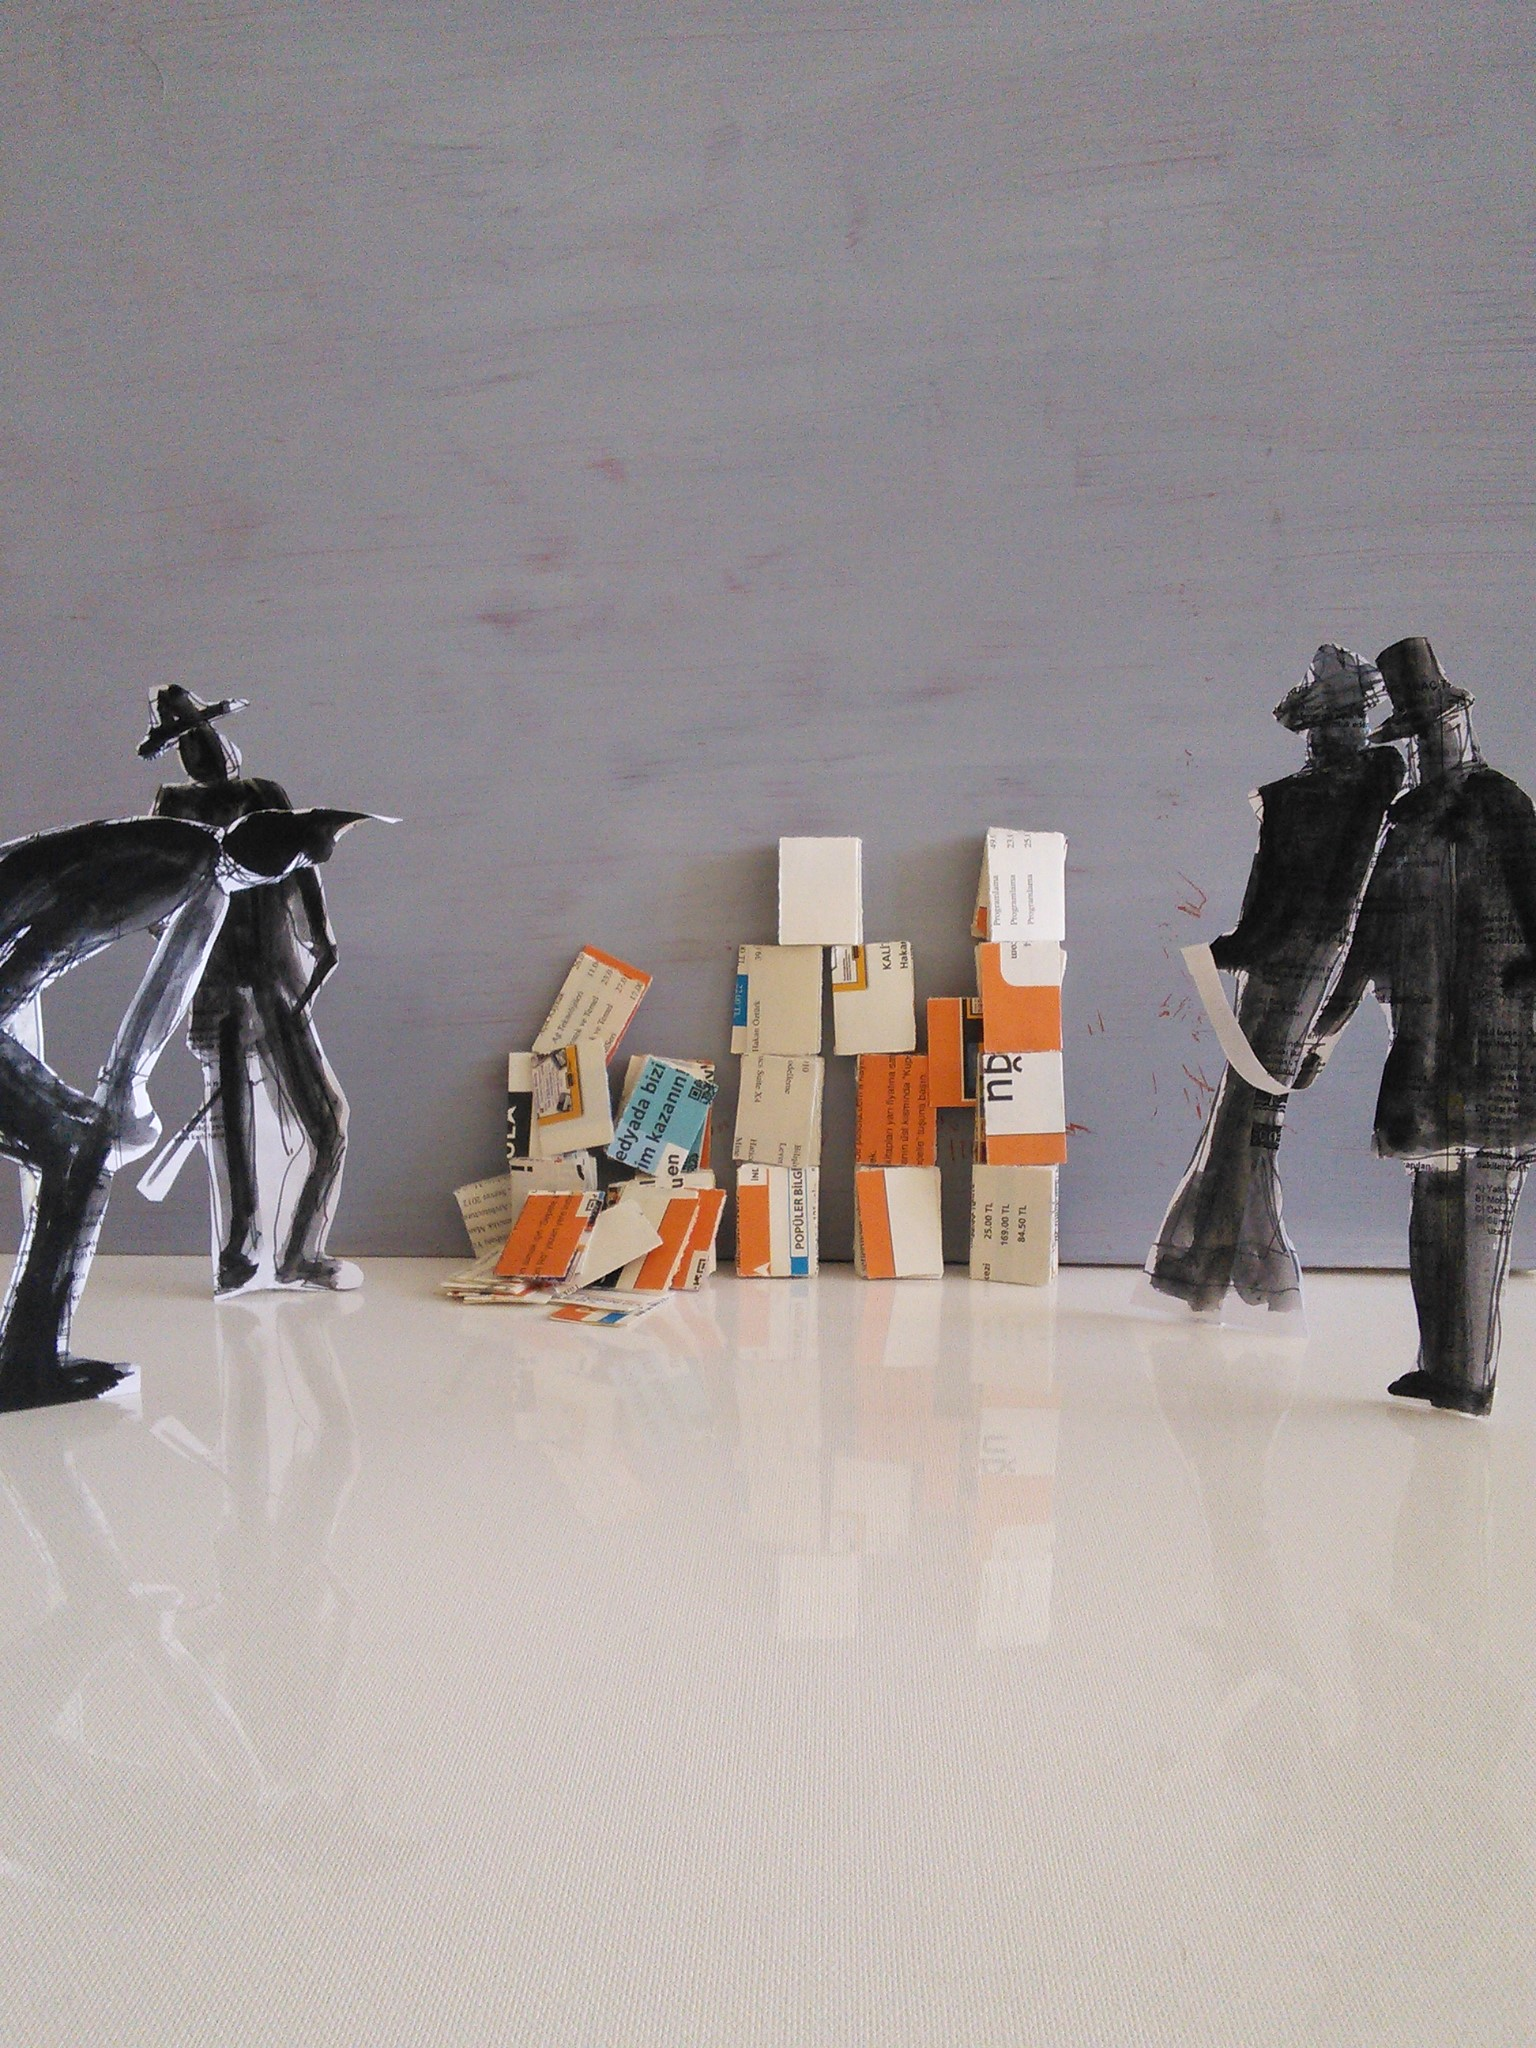
\includegraphics[width=\textwidth]{project_graphics/exhibition1.jpg}
    \label{fig:exhibition1}
  \end{subfigure}
  \hfill
  \begin{subfigure}[b]{0.31\textwidth}
    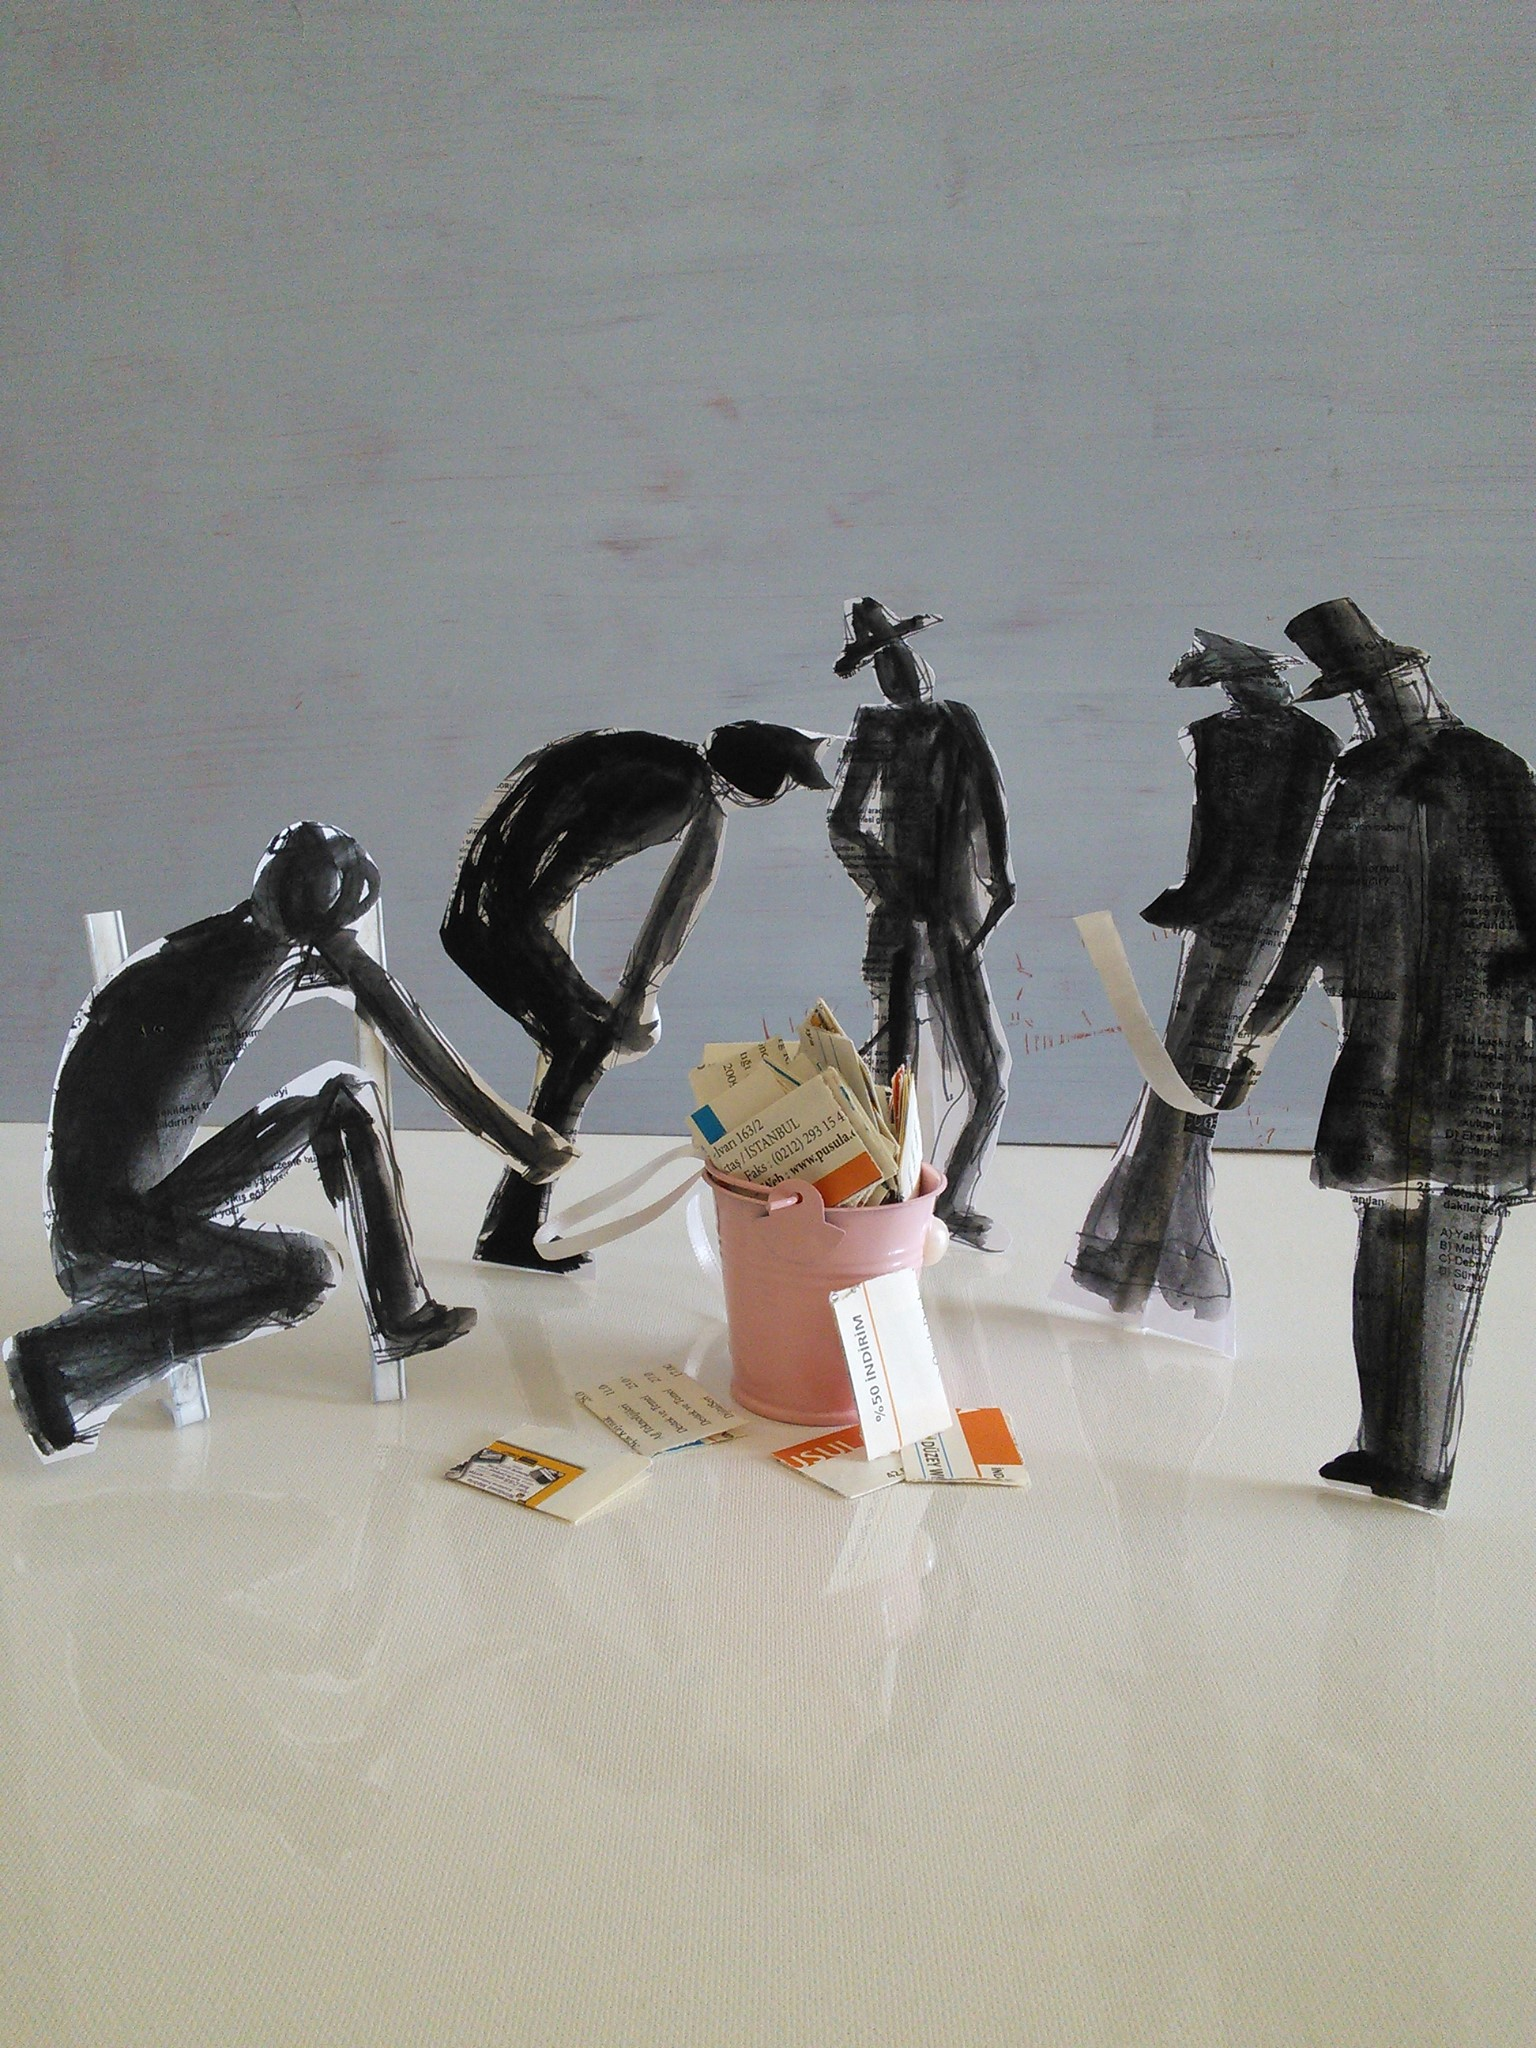
\includegraphics[width=\textwidth]{project_graphics/exhibition2.jpg}
    \label{fig:exhibition2}
  \end{subfigure}
  \hfill
  \begin{subfigure}[b]{0.31\textwidth}
    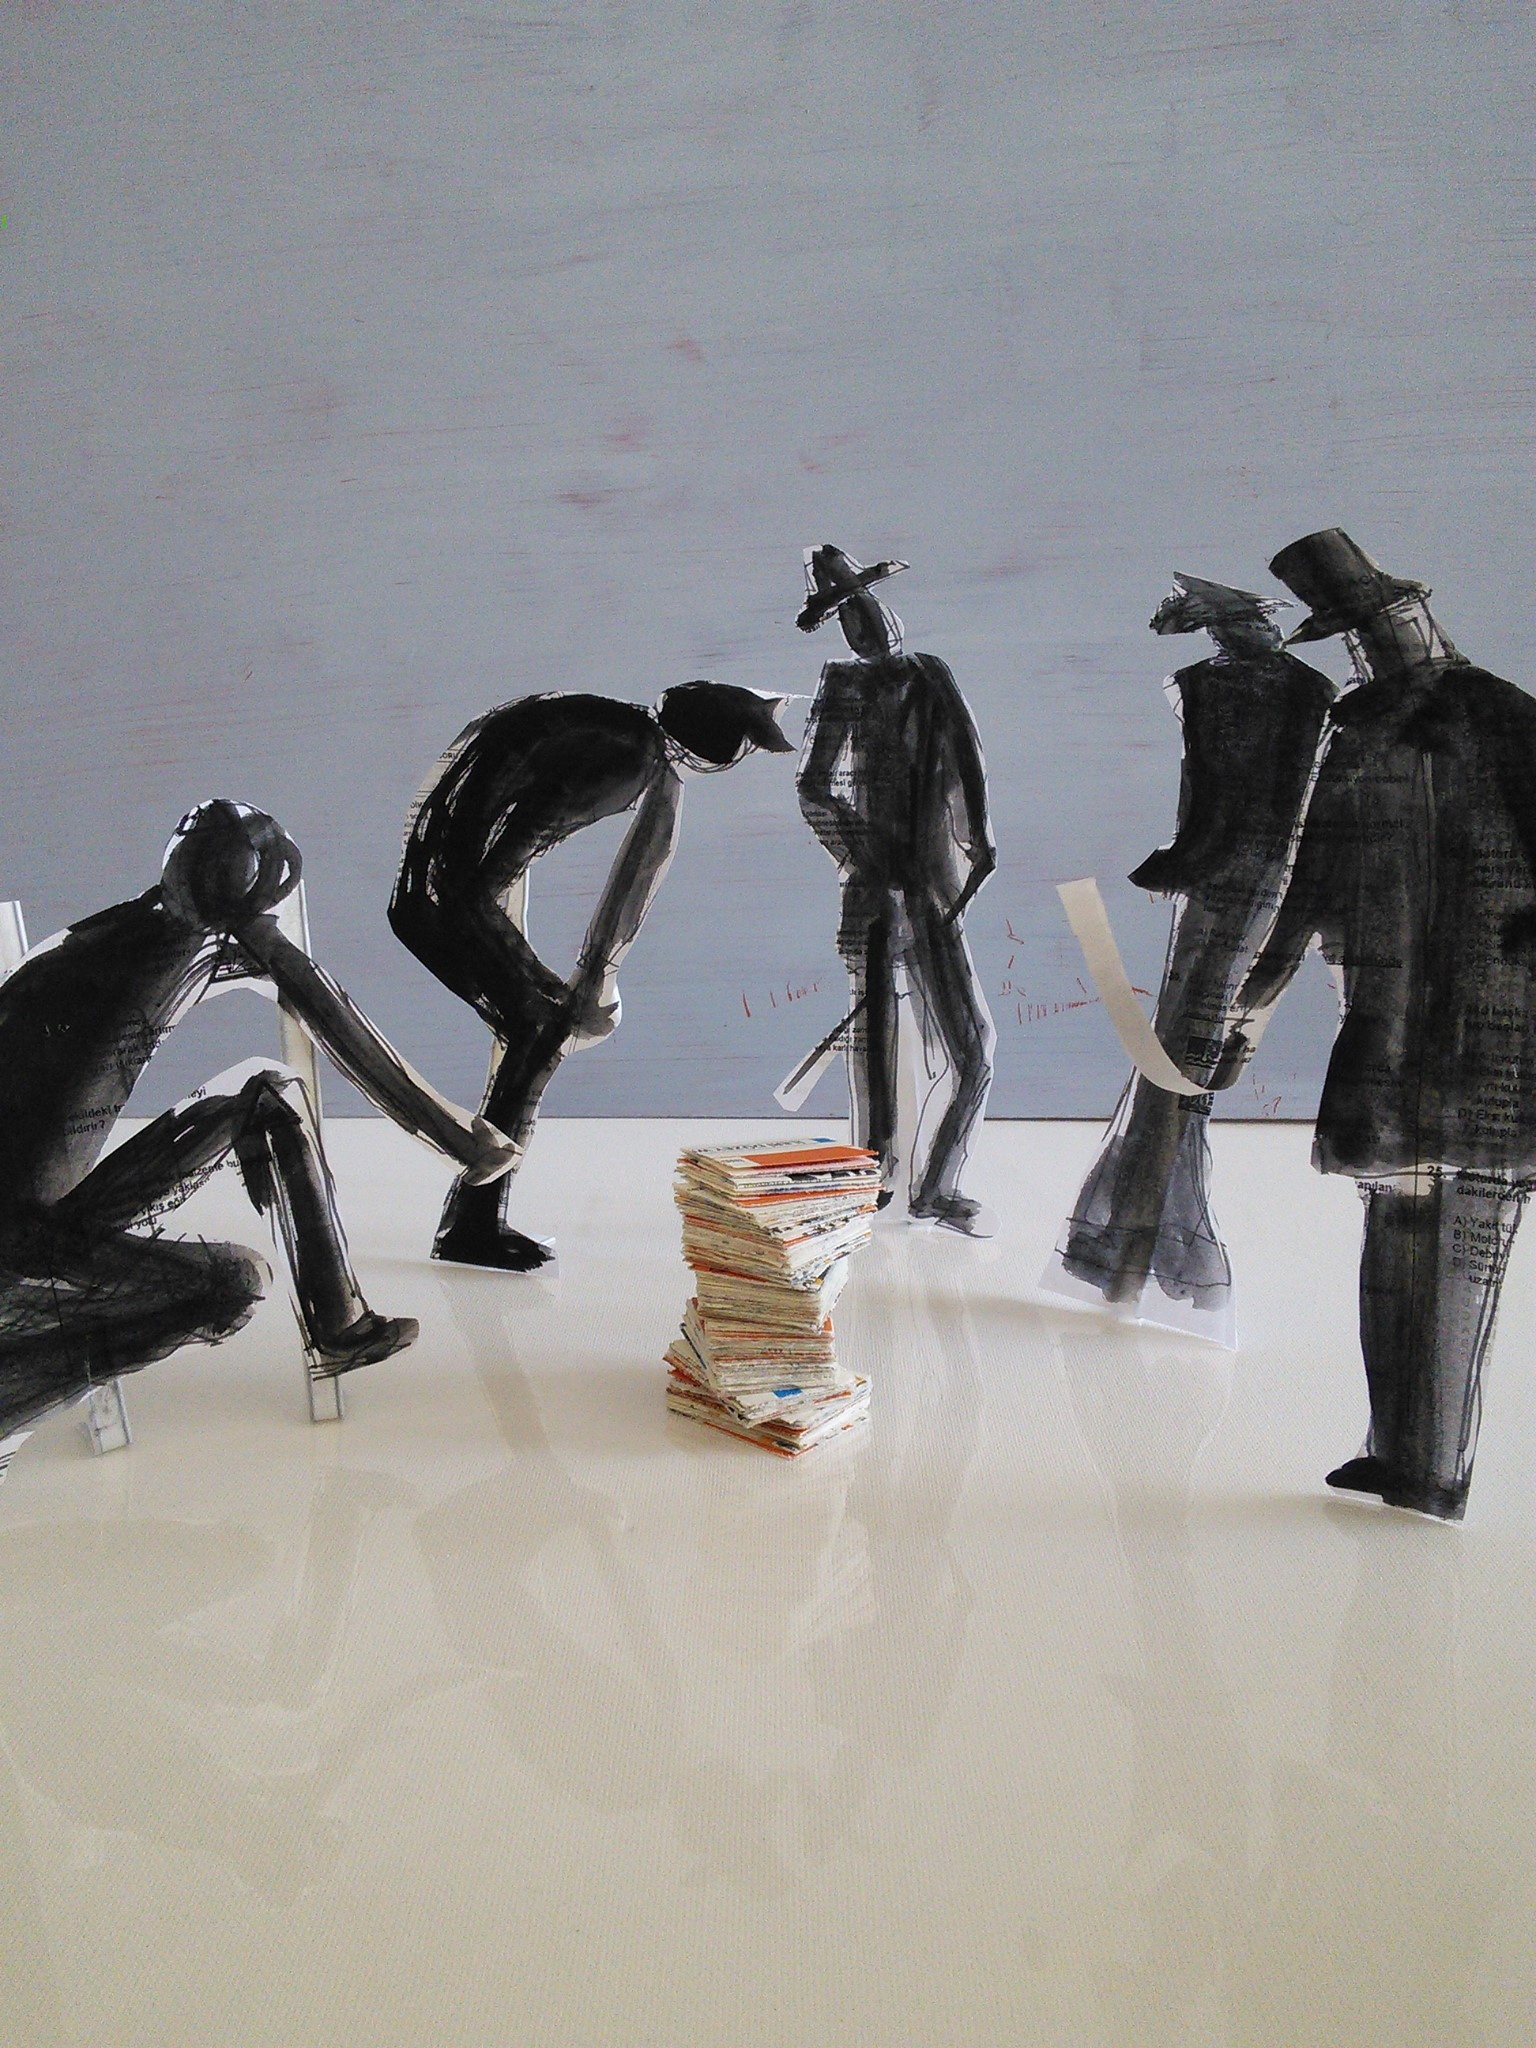
\includegraphics[width=\textwidth]{project_graphics/exhibition3.jpg}
    \label{fig:exhibition3}
  \end{subfigure}
  \caption{Installation experiments with models}
  \label{fig:exhibition}
\end{figure}

They were early interpretations and ideas. I imagined an exhibition environment to place notebooks. Different placements were tried. All of them looked like a sculpture. I have inserted no special meaning as sculpture to this objects. I also afraid that people will not interact with them and look them away. My purpose is give people. Aim is to spread the idea by making something useful from trash. Increase diversity, encourage people to embrace the trash.

These experiments showed me that I need to place them to the locations where people frequently visit. It must be inside of the life. As it is collected publicly it must be showed publicly. Thus the project can reach more audience. It will spread and can be showed in different contexts. Notebooks can move with people.

% TODO boxes and wooden cases
To hold notebooks together I made several small boxes from discarded card boxes. Notebooks were put inside of them.

In the production phase of the boxes, I discovered that my folded notebooks are fit into the many card boxes. In other words dimensions of them are not very different. This property of items make my production more easier. It shows that industrial system supports the reuse of the object with less effort in this way.

% TODO Rubbish Theory showing off.

% TODO [Why giving away?] Felix Gonzales Torres, Unlimited Editions.

% The \quotes{Untitled} series of Felix Gonzales Torres inspired me a lot when deciding giving notebooks away. He has created variations on the theme of the “stack,” which consists of “unlimited” editions of offset prints. Visitors can take a copy of them. 

% TODO insanlar bu defterleri neden alsınlar.

% [Website]

% websitesinde amac bunlari anlatabilmekti. 
% Anlattığım bir çok şeyi sadece deftere bakarak anlamak mümkün değil ve ben bunların insanlara ulaşmasını istiyorum. buradaki seçeneklerden bir tanesi site ile onlara ulaşmaktı. temel sebeplerden bir tanesi bu mediumda ben tecrübeliydim. for the smaller parts what is written on them can not easily understandable. To realize what is the message is you have to bring together all of them again. But It is not possible, therefore website is a very good solution for them.

Beyond all of these for the audience the story of the collected materials is a mystery. Audience are not aware from all of these written in this thesis. I want to reveal the act behind these notebooks. However there is a lot information that can not be fit into the pages of notebooks. For that reason such problems can be clearly solved through a website that store the records of notebooks and collected materials. People can visit the website anytime. Further I am comfortably and confidently fluent in coding and web development. Therefore it is more appropriate for the scope of this thesis.

Notebooks will be given away. They will continue to flow between people. There is a possibility that notebooks can be trashed again. However vice verse is possible. In other words they might turn to durable objects as mentioned in Rubbish Theory. At this time, decision belongs to people. However website serve great functionality here. While the notebooks have potentials to be rubbish, records of them in the website are preserved.





%
%
\section{Parts of the Final Work}
As also can be understood by the previous section the project introduced in this thesis have different parts. Each part support the other. They are connected with each other. Different parts lead different inquiries.





%
%
\subsection{Notebooks}

Notebooks have been used for different purposes such as drawing, writing and recording, ideas or memorandum by many artists, scientists, and thinkers through the ages. Further same exist for me and people around me. Although the digital alternatives of it paper maintains its place in the community.

Through this project handmade notebooks are produced from discarded paper. They are impure, imperfect and different than usual industrial notebooks. They still carry the traces of previous usage. Every one of them have different stories. Combination of various pieces offer new interpretations of writing.

There are different types of notebooks regarding their color, shape, size and combination. They are simple, imperfect and different than usual industrial notebooks, but more importantly they are from trash. Every one of them has a unique serial and with that serial the (hi)story of it can be viewed.

% Meaning of stories behind the process
There are different stories behind the objects. I try to record their stories (by photography and taking notes) but some of them were not possible. However I still use them in the work because even if I missed their story, with their materiality reveals their history. It still has a history but needs to rewritten. Maybe forgetting all the history maybe creates different notebook.

Every notebook has unique serial and with this it can be tracked down when it was produced and which materials are used production of it. Serial is generated through the first letter of composed material. 

Giving name is another hard topic for me. However point out the story behind the notebooks and properties of it. These names gives clues about how they are combined what they represent, defines the aspects of them. Name of the paper can be related with this place and related with the meaning. These names captures the memory of notebooks. However for one series I borrowed the idea of nonsense word generation from the Kurt Schwitters. Similar to the the production of the nonsense word merz I decided to name some of the notebooks a nonsense word. There are notebook series that have a name. Here are the name of notebooks and their story:

\textbf{Puzzle.} Papers inside of these notebooks are cut out from very big and long banner (see figure \ref{fig:Banner_1}). Every piece is a part of bigger banner. Pages of paper is similar to the pieces of puzzle. All of them are composes the banner. However they are cut out and give away combining them is not possible but the image of the original one can be viewed on the website.

It provides unique layout for writing and I strongly think that all the notebooks after used have strong visual impact.

As mentioned previously the objects are bring their history. They are not blank, they are heterogeneous and hybrid. It can be one of the examples of this argument. 

\textbf{Reunion.} These notebook's pages are collected from restaurant Varuna Gezgin, in Ankara. We went there to meet some friends after long time. One of them was coming from Australia, the other one was coming from Norway. They were my friends from the university. We united again at this restaurant. The place has also similar story. Their founders and workers travel around the world. It is a popular restaurant of travelers. The decoration of that place contains a lot of items collected from different sides of the world. The concept of the place and our meeting perfectly matched. Same exist for the papers actually, they are separated from big paper rolls in the factory and by the action making notebooks they are also reunited again. These notebooks represent my memory about the place.

\textbf{Secondhand.} It can be thought that these notebooks are second hand objects. Used by someone else and still appropriate for reusing.

% TODO burada bir isim uydurmak gerekli.
\textbf{Daro.} For some of the notebooks it is not obvious to name them. At this point approach of Kurt Schwitters provides me a way. He generated his frequently used word \quotes{Merz} from an advertisement. It is a nonsense word and used in most of his works. I followed what he did and generated a word from the papers that used inside of the notebooks. I use the word \quotes{Daro} extracted from \quotes{Vardaroma Dondurmacısı} for the ones whose story are not obvious and significant.





%
%
\subsection{Exhibition}
Especially it is the most hard topic in the development of the thesis. To find an appropriate place for the notebooks is great challenge for me.

\textbf{Public space.} The reason why select library is there are small papers to write down the location of books. Libraries are places that things are reused. Books are used by many people. It is place of sharing culture. Books are shared by all the other peoples. Public space. It is place that students from different department use the same place.

Notebooks are placed where people frequently visit such as computer desks.

\begin{figure}[!tbp]
  \begin{minipage}[b]{0.48\textwidth}
    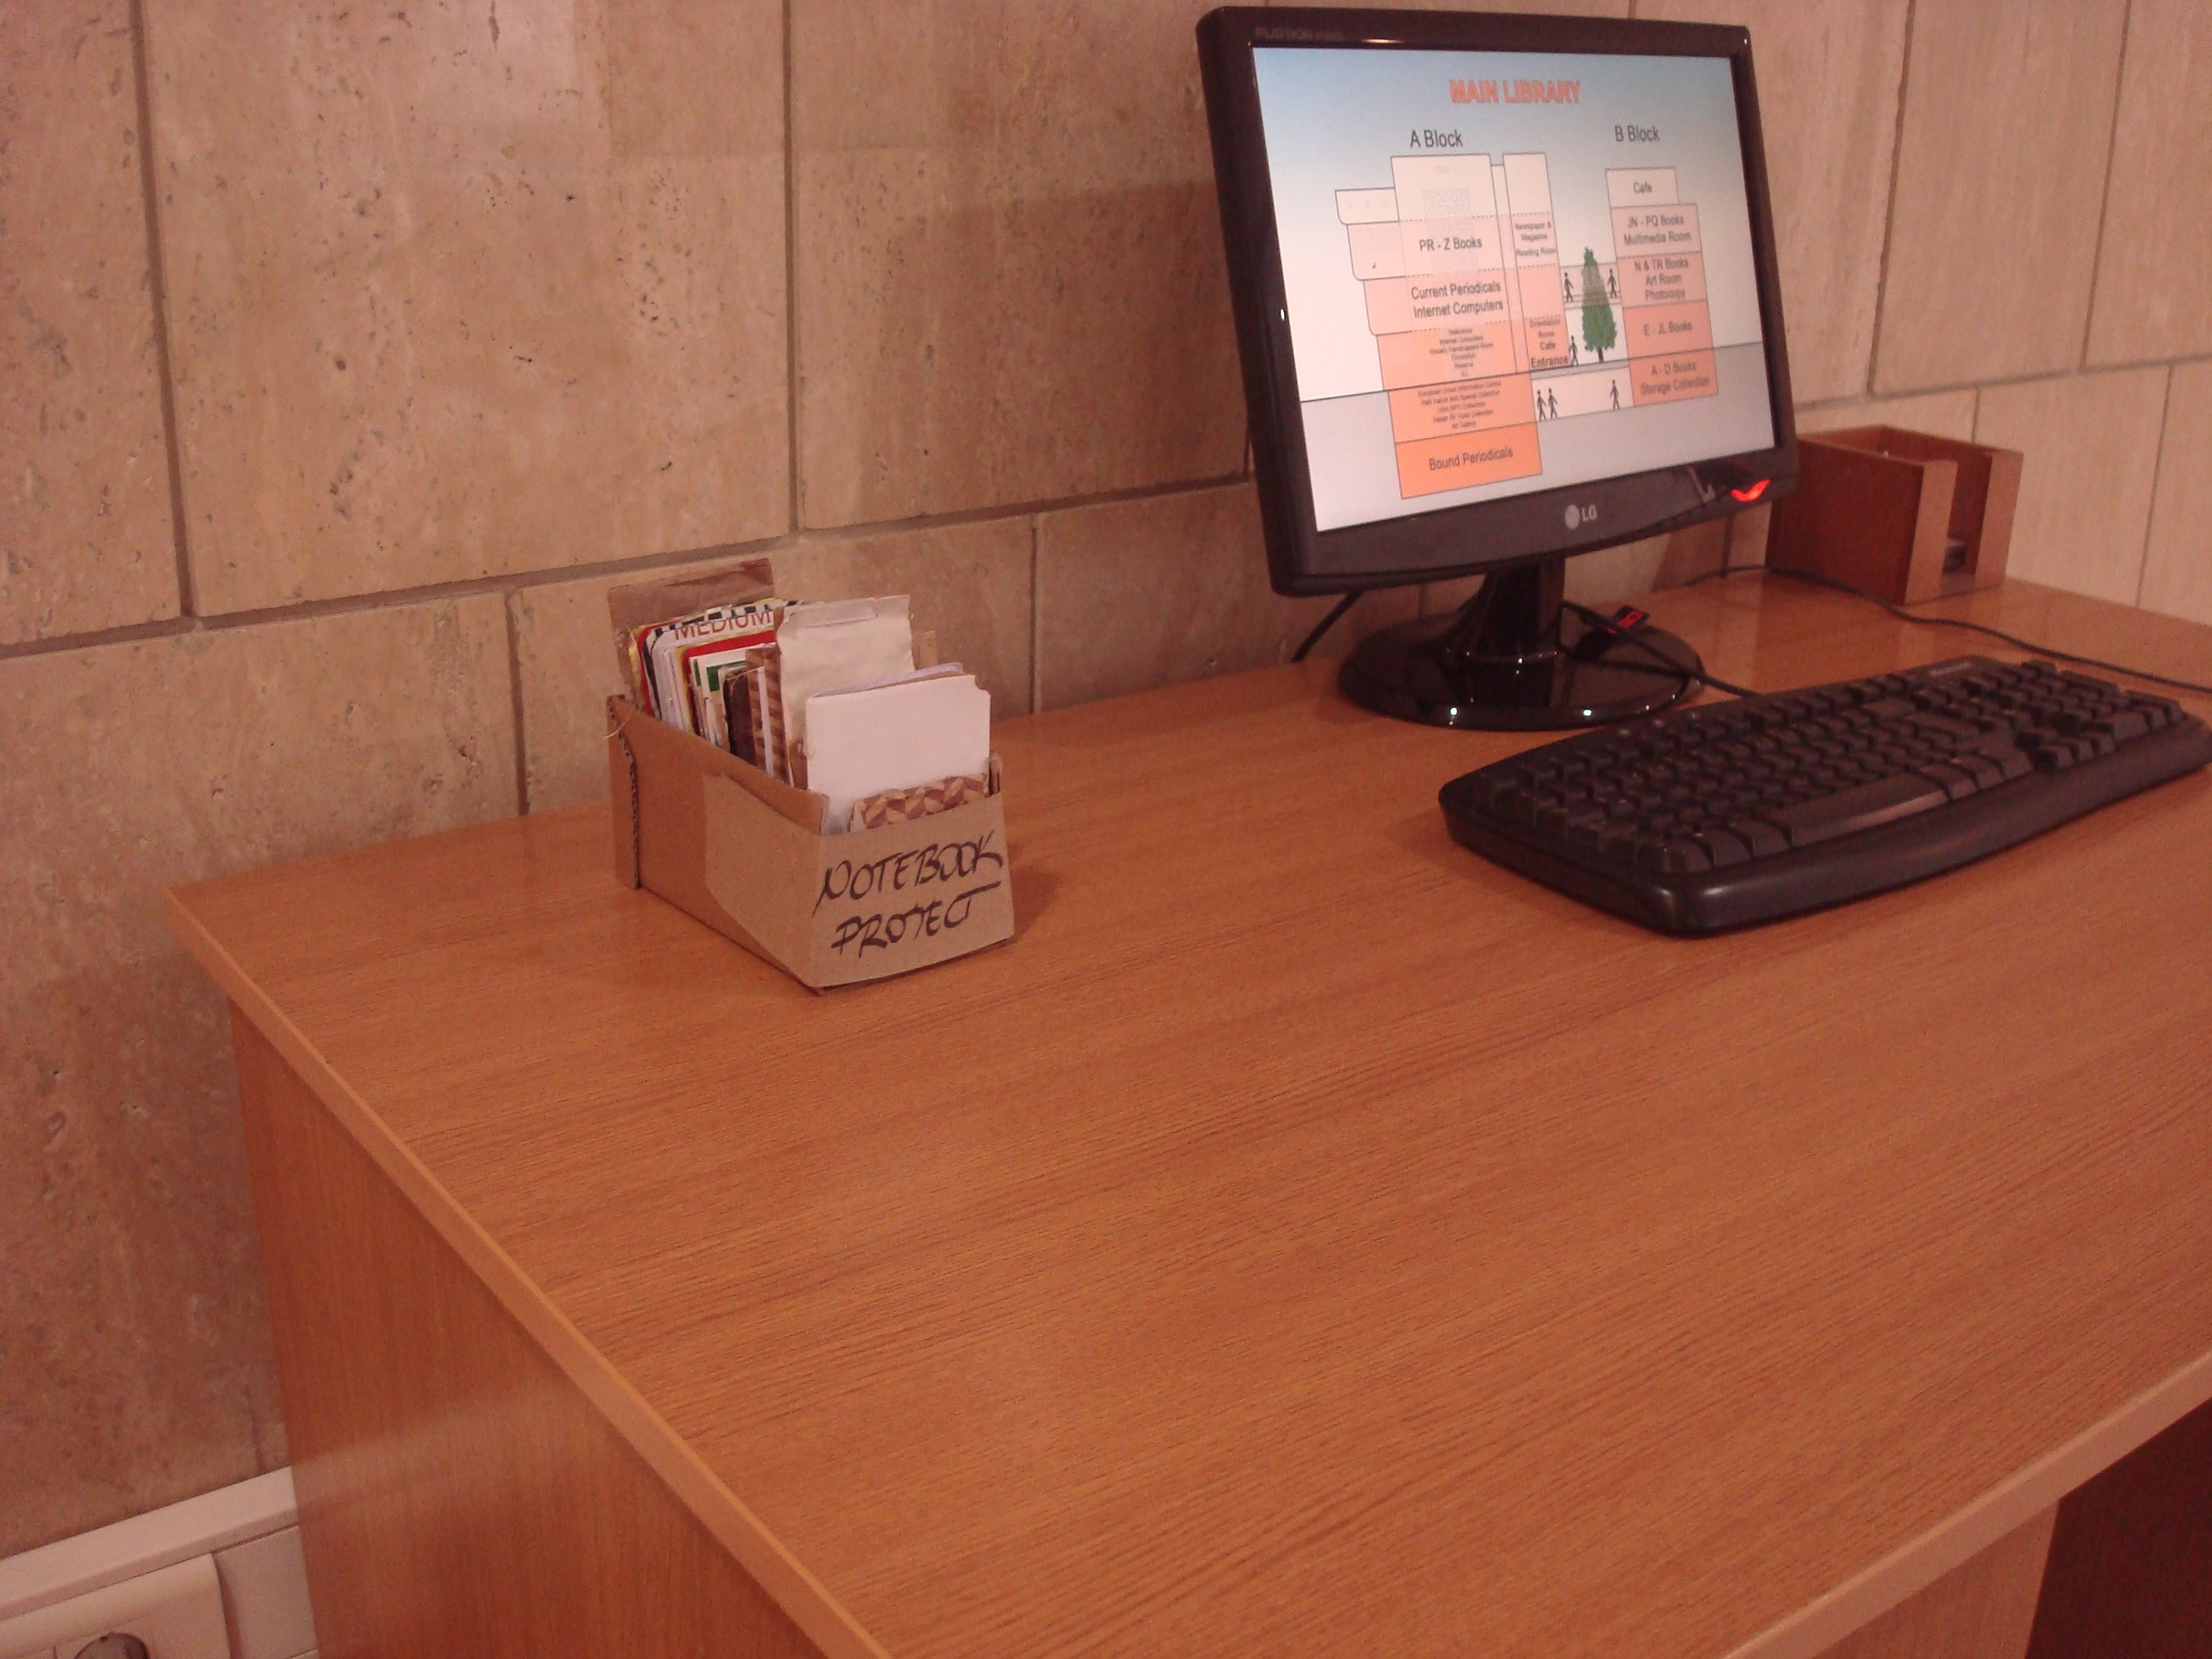
\includegraphics[width=\textwidth]{project_graphics/bilkent1.jpg}
    \caption{Library}
    \label{fig:BilkentLibrary}
  \end{minipage}
  \hfill
  \begin{minipage}[b]{0.48\textwidth}
    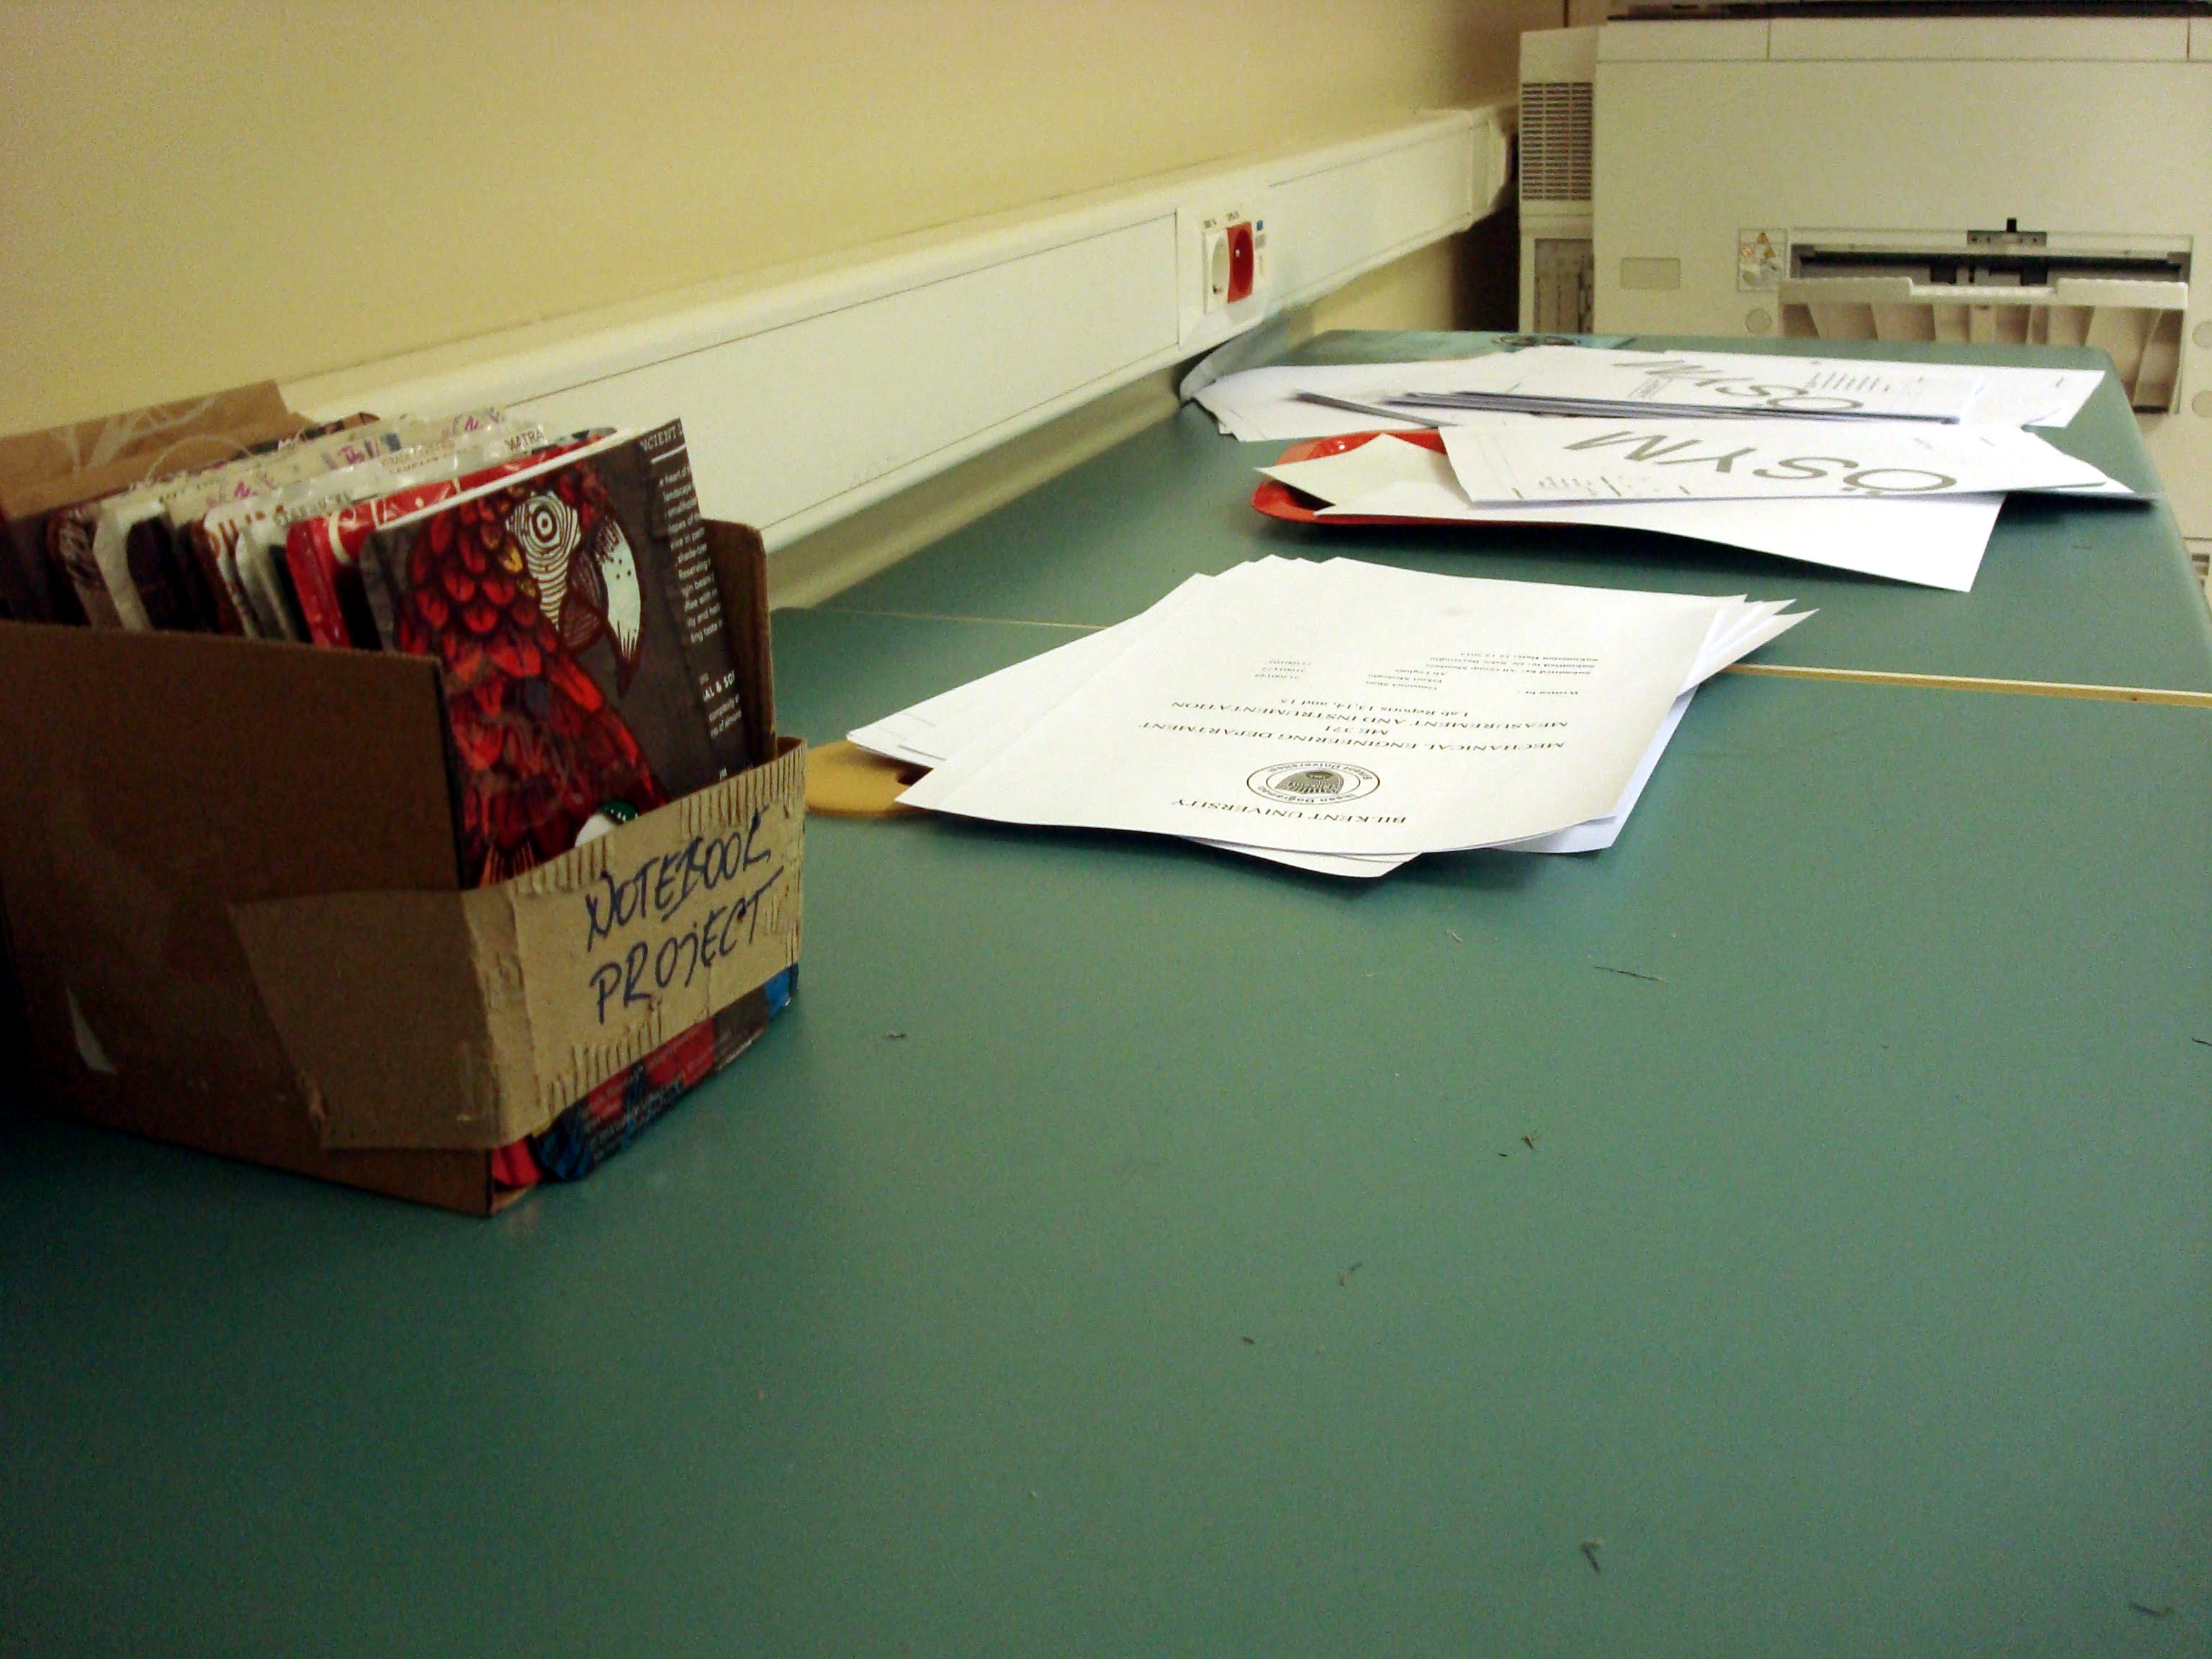
\includegraphics[width=\textwidth]{project_graphics/bilkent2.jpg}
    \caption{Computer Laboratory}
    \label{fig:BilkentLaboratory}
  \end{minipage}
\end{figure}

% su anda sadece bilkente yerlestirildi. Odtuye daha koyamadim. Neden koymadim. Nicin koymadim. Koymali miyim?

% bir çok insanın ortaklaşa kullandığı bir alan. kesişim alanı. bir tanesi de özellikle zaten toplanan yer. insanların defterlerle karşılaşmalarını istiyorum.

% Selected places are frequently visited by people. Shared places. 

% Torun
Through this project another exhibition alternative is thought. In the notable museums and art galleries there are gift shops that people can buy souvenirs. Often they are mass produced imitations and replicas of well-known artists work embedded various objects such as cover on the notebooks. At this point I image an art space you can buy these types of items freely. In other words alternative to the existing approach this types of gadgets. Another alternative interpretation can be giving away different that the industrial items such as notebooks from trash as in my project. For this type of approach Torun is a great place to show my notebooks and give them away. Torun describe itself as a place for free place for sharing art. Open to everybody. Makes open call to the any artist. There are no security cameras on this gallery therefore no one is watching you at there. This idea shared with Torun and they accepted it. However Torun will opened after 14th of the January currently I just took some photos at there.

I used wooden market boxes to lift up them from ground to more reachable height. It is hole body of stand to put notebooks. Notebooks are placed on the top box and below them I just put the collected items to provide for those who want to make their own notebook. People can get them both. Further it reveals the process of the production of the notebooks. Shows the previous state of the materials.

\begin{figure}
  \begin{subfigure}[b]{0.48\textwidth}
    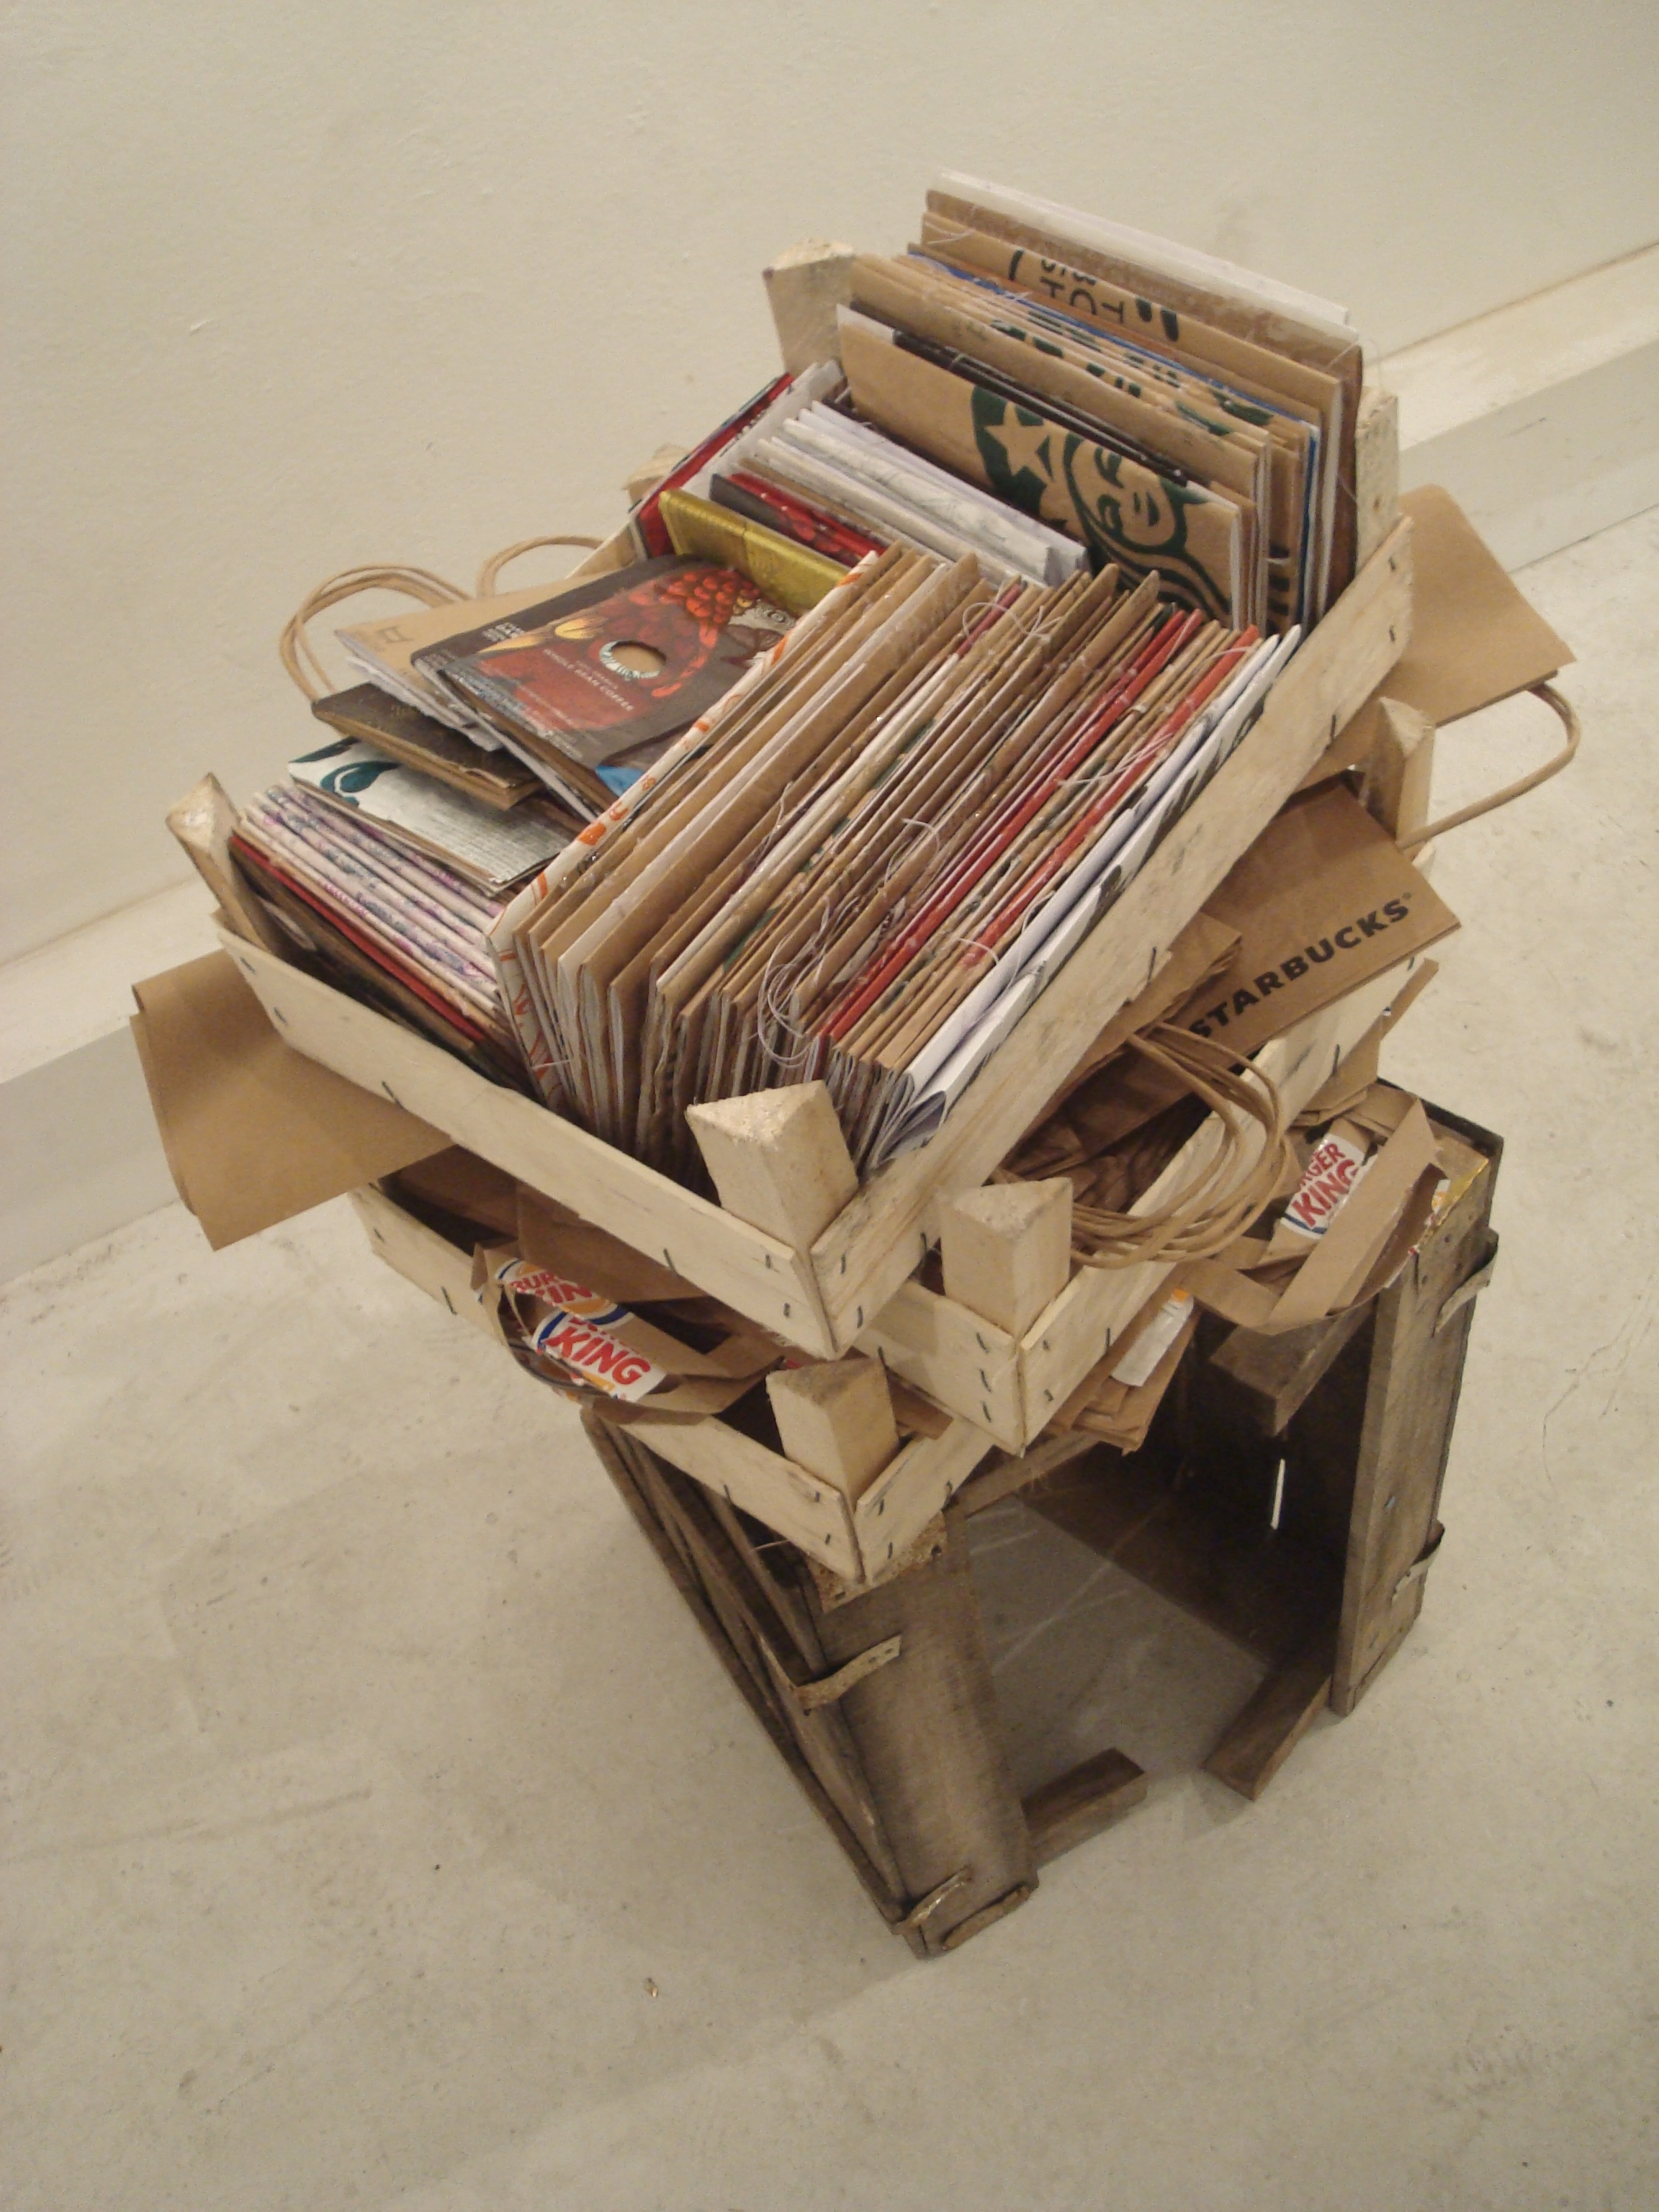
\includegraphics[width=\textwidth]{project_graphics/torun3.jpg}
  \end{subfigure}
  \hfill
  \begin{subfigure}[b]{0.48\textwidth}
    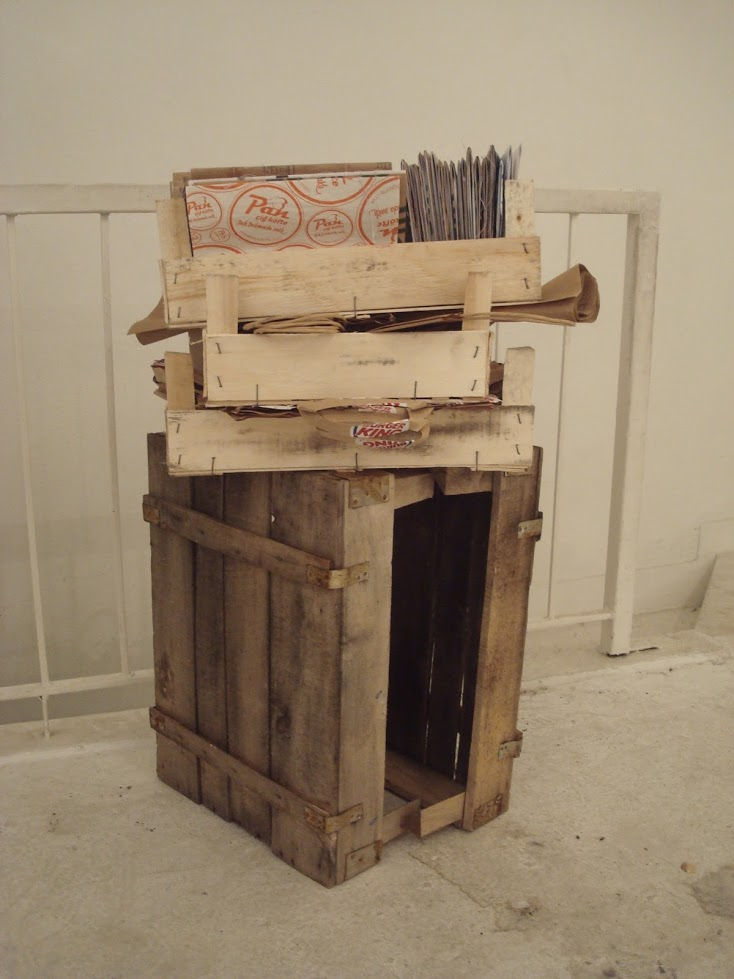
\includegraphics[width=\textwidth]{project_graphics/torun2.jpg}
  \end{subfigure}
  \caption{Sample placement at Torun}
  \label{fig:SamplePlacementAtTorun}
\end{figure}

These are example placement. The exhibition event is not held. It is only decided. These notebooks are not only exhibited there, but also I will turn it to an workshop that continue to produce notebooks and show people to how to do it. Maybe they will join me in the production of notebooks. They can bring their items and transform all together. We can share our ideas and thoughts with each other. 





%
%
\subsection{Website}
Finding a new place to the discarded items is one of the main purposes of this project. Not only it finds a place in people's life again, but also it finds another place in the digital space.

Mainly website displays the (hi)story of notebooks. It contains a section for how notebooks are produced and the story behind it. The purpose is to record the creative process and share with others. Revealing the process is significant to demystifiying the truth about the project. It makes it more clear that the object used here is actually transformed from something else. People can access to images and descriptions of notebooks. All the development process of the project will be revealed in this website. Will contain list of collected materials. 

Into the notebooks a sticker which contains qr code and short description with the address of website is pasted. People can able to reach more information through this reminders. 

\begin{figure}[h!]
  \centering
  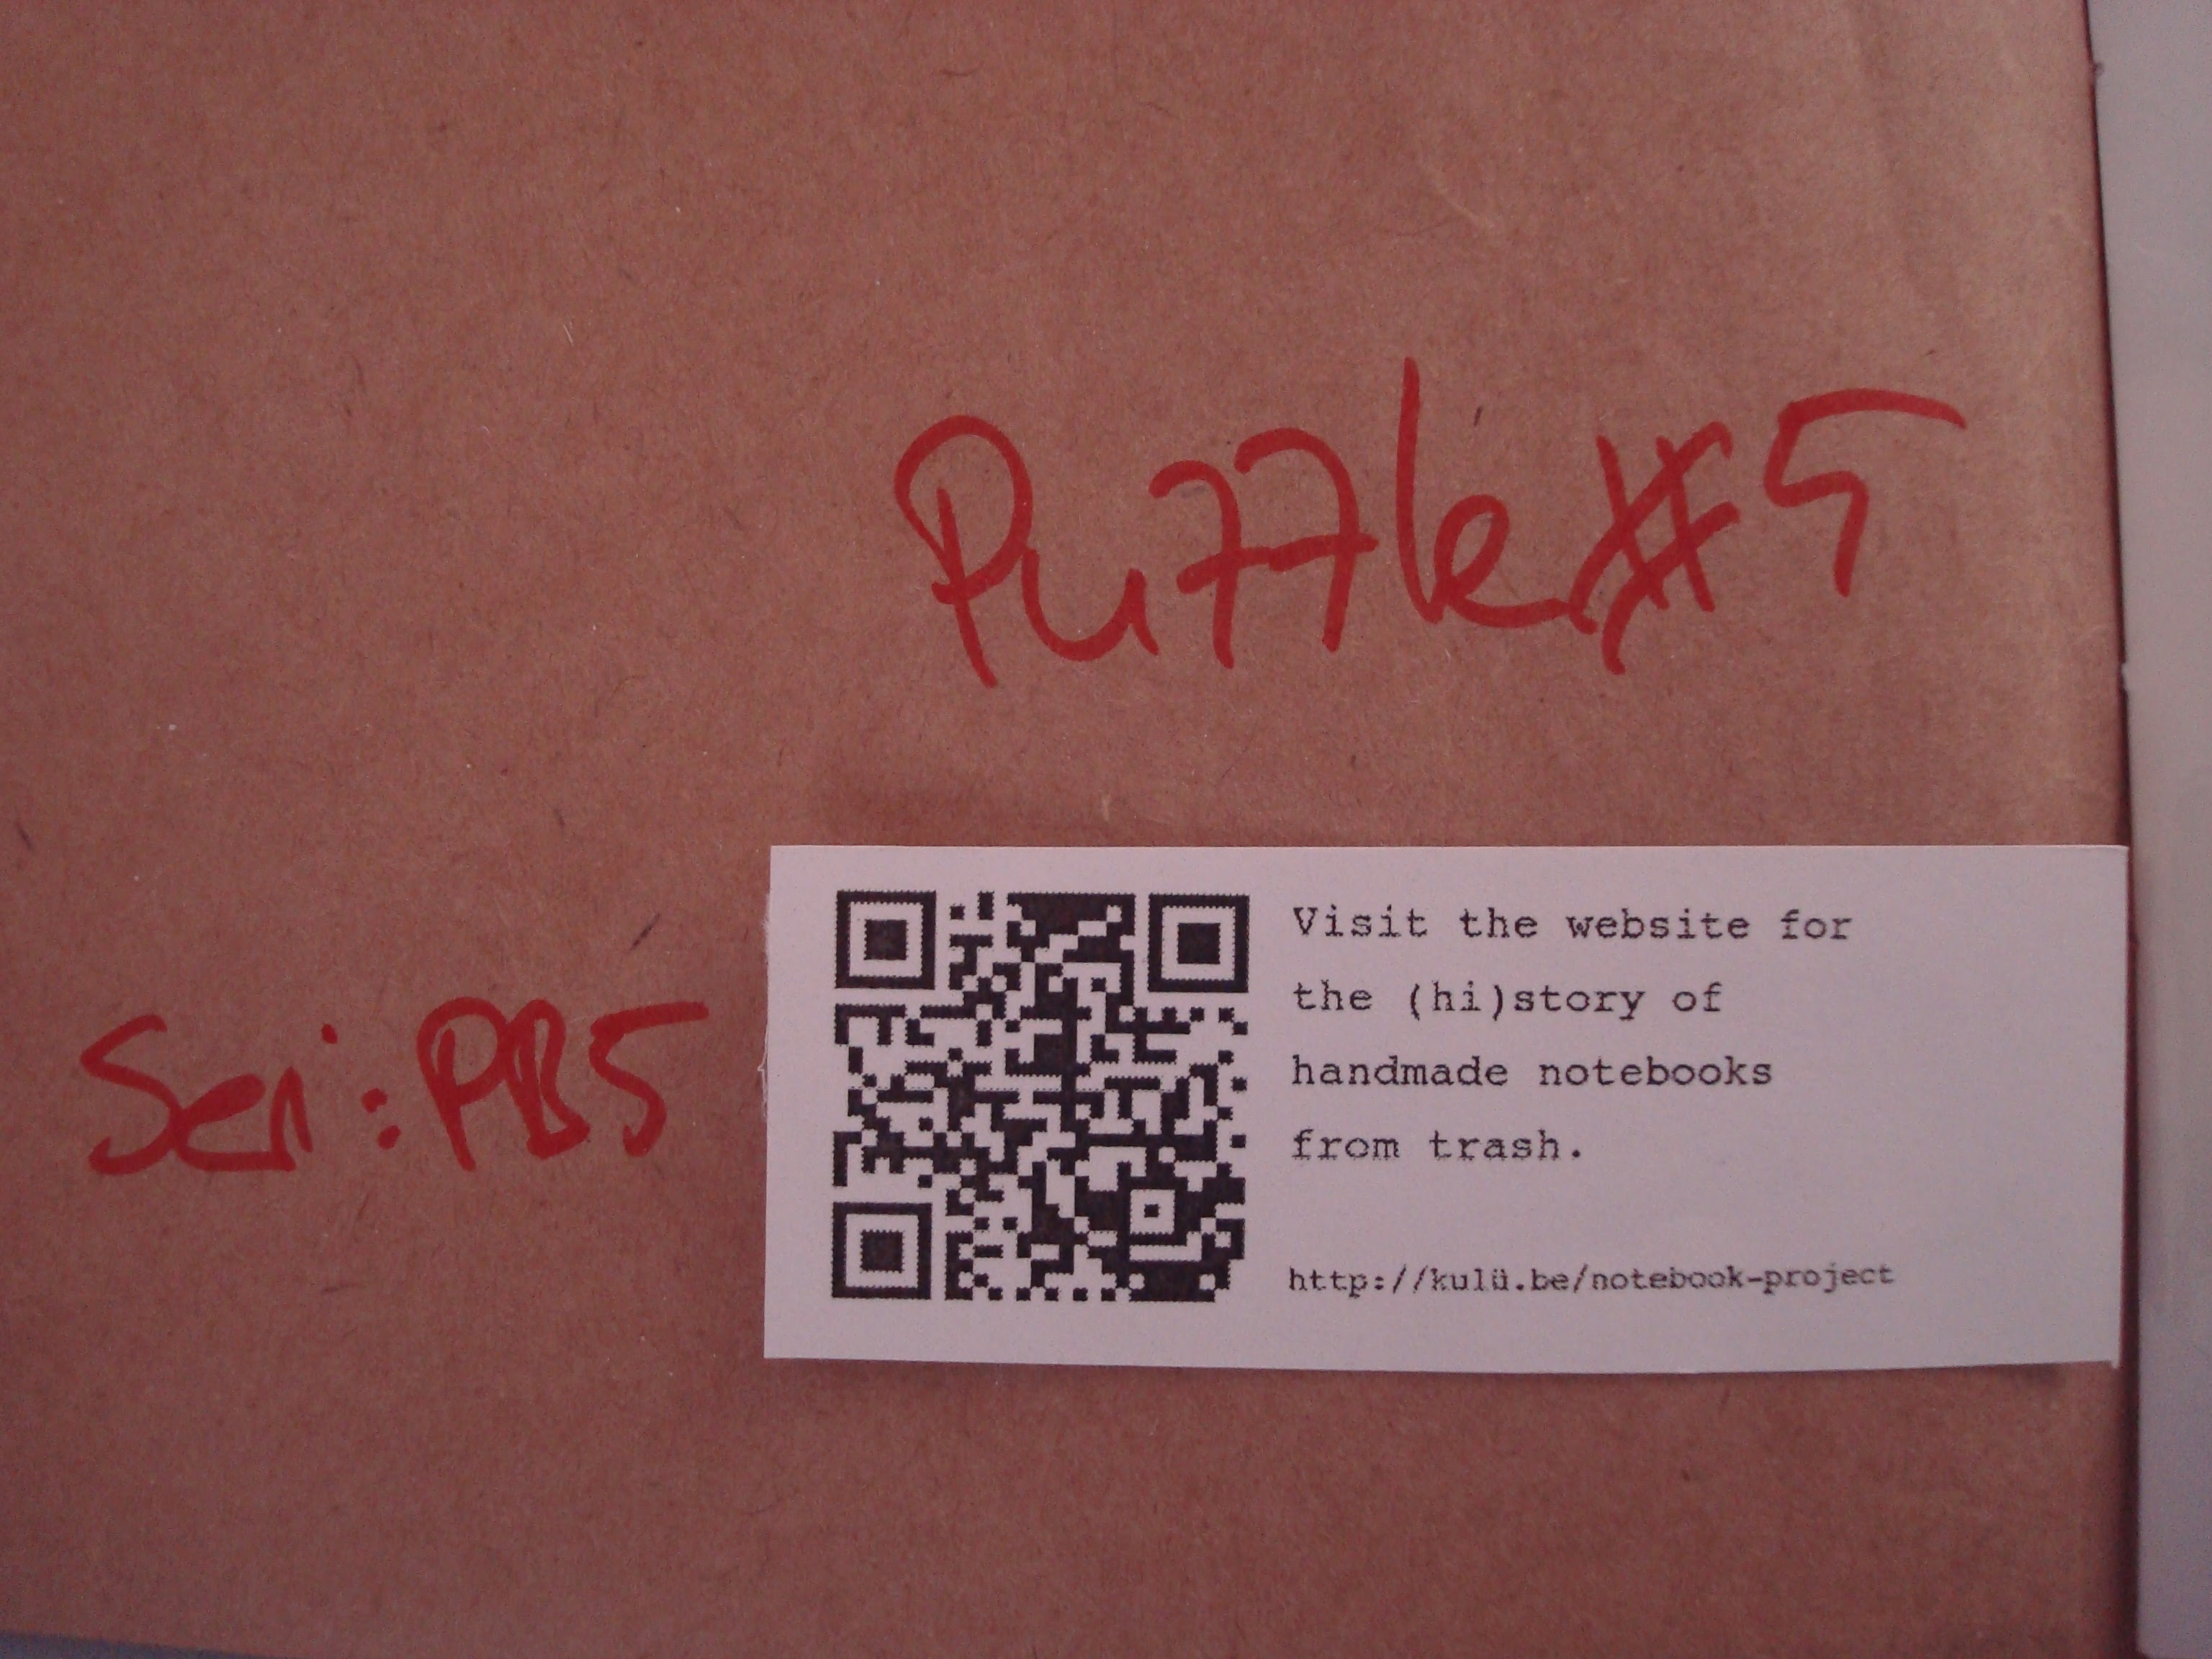
\includegraphics[width=1\textwidth]{project_graphics/qr_serial.jpg}
  \caption{Sample of QR code and notebook serial}
  \label{fig:QR}
\end{figure}

Website is a place to track the journey the notebooks. Transformation of it does not completed. It always continues. Therefore a website that anyone can reach and share their progress via website will show their evolution in time. Anyone can later discover how they turned to new things.

As I leave notebooks different places I do not have connection with people who take them. This website also will help to share peoples ideas about the notebooks.

Maybe it can be thought that there are different methods to accomplish recording and sharing the process. In a gallery on a single table or a room it can be succeed. However it like the idea that website can evolve by time as this work evolve in time. I think it matches perfectly. This is not a finished work, it continues and so the website also.

%SketchBook Project is also inspired me a lot especially in terms of website. This project provides a platform to people in order to share their works with other people. It contains lots of works from all over the world. Full of creativity and showcase of richness of people's expressions on the small notebooks. My work can be considered as a sketch book project through trash. Sketches or only creative progress is not the only consideration. You can send your lecture notes.

Website can be accessible through this address \url{http://kulu.be/notebook-project}. Domain name kulu.be belongs to me and project placed under a directory of it. Website is coded by me with the common and trusted open source libraries and frameworks. Its code also available at this address. Site is served from GitHub pages which provides free website hosting. Pages are generated by Jekyll which is a static website generator through it some repetitive works are can be easily automatized. 

Through the website people can be able to subscribe to the newsletter to get updates about the project. People can be able to add their comment to the website. How they are using their notebooks will be showed through it. Website will function as a platform to get into touch with people. From one point of view website can bee seen as a visitors book.

In the future all the discussions and research can be moved to the website that people can reach more information about the subject. This thesis and presentation will also be added to the website. 

All the progress up to now forms the core of the project. However it is not limited with it. The project will be continued after this thesis completed. New features will be added to the website. In the future it is planned that through the website people can be able to request to get notebooks. Thus notebooks become more accessible to the other people. Moreover notebooks done by others from trash can be added to the website. Beyond notebooks various objects transformed from trash can find a place in the website.


\chapter{CONCLUSION}





%
%
\begin{singlespace}
\epigraph{If I seem to be over-interested in junk, it is because I am, and I have a lot of it, too --- half a garage full of bits and broken pieces. I use these things for repairing other things\ldots But it can be seen that I do have a genuine and almost miserly interest in worthless objects. My excuse is that in this era of planned obsolescence, when a thing breaks I can usually find something in my collection to repair it --- a toilet, or a motor, or a lawn mower. But I guess the truth is that I simply like junk.}{\hfill---John Steinbeck, \textit{Travels with Charley, 1962}}
\end{singlespace}






This research began through a desire to understand more about the subject of rubbish in art practice. It attempts to figure out the transformation of trash through the artistic practices. It presents different uses of trash and approaches in the context of art. Example artworks suggest that it provides to artists wide range of possibilities. In other words it can be viewed as a source of diversity.

This thesis takes a rather different approach to the discarded objects. It looks to philosophical ideas, theories and people’s experiences of things in throw away culture.

People’s evaluations of what is trash and treasure are both content and context dependent and are not fixed values. The line between them are blurred in the explored practices and works of art. Indeed, temporal value judgements of ’rubbish’ and ’art’ are often at the core of such art works. The analysis of selected works methodologies and approaches show that trash is fluid, and value indeterminate, and are often determined by context and personal subjectivities. 

This thesis analyzes the basic principles and approaches in the act of transformation of trash. It provides examples of artworks that inquiry the issue of trash in various dimensions. César shows that trash is not only found in dumps but also can be found in museums. Dong shows that how trash is essential for some people to hold on the life.

Whatever the reason of discarding objects the alternative if it showed through the works of artist and the thesis project. In the project aimed to create new possibilities from trash. The usage of discarded paper bags, packages in the project provide audience new interpretations of the materials and meanings. On the other hand transforming discarded papers to notebooks evolved from a hobby to research grounded framed project.

The project developed in the scope of the thesis open to further developments. Content of the web site will expand in time. New notebooks from various discarded papers (in terms of location, meaning and purpose) will be compiled. Upcycling of trash will be extended to the other waste materials in addition to the paper. However research, practices, methods followed in this thesis form the basis of all these.

There are lots of points to approach to the trash. This shows that the richness of this topic. The scope of the research leaves many more areas untouched. There is much potential for further work in this subject. Certain major avenues have not been discussed in depth, not because they are irrelevant, but because there simply has not been time or space to explore them in sufficient detail and some reduction in scope has been necessary to be specific in such a wide field.

For instance, research can be extended to the notion of waste in the digital realm. Both digital notions like spam emails and  effects of digital devices on e-waste need further investigation.

The focus on waste material in art in this study has also largely disregarded waste of other non-material concepts such as time. Wasting time is another significant area of exploration.

As mentioned the value and meaning of objects changes from people to people, from society to society. Therefore more focused research can be conducted to analyze the local practices of transformation. This thesis work is formed in the English language but local languages have potentials to reveal the various concepts and practices of trash.

Different selection of works and their analysis and relation between them will form another thesis which identifies another dimension of trash.



% Bunu landfill orchestrada kullan
% FROM Book: Recycled, Re-Seen: Folk Art from the Global Scrap Heap
%\summary{Ironic}
%\comment{IRONIC, maybe added to results of transformation, reusing trashed items in different contexts.} This misuse the detritus of the industrial age has been described by western theorist as ironic. the irony is often embodied visually and conceptually. opposite of natural use, expected perception. for example making something from nothing or turning trash into treasure. By juxtaposing different materials changing context and place. 

% TODO From Beautiful Trash Art and Transformation BY PAOLA IBARRA, ReVista
%Recycling has always been a common practice in the arts at least at a non-material level. From creating a world of words in literature, to rhythm and images in poetry, sampling in hip hop music, representation in the visual arts, or editing the illusory continuity of a film, art implies taking disparate elements (ideas, images, references, objects, etc.) and putting them together to form a new whole. Take and put. De-contextualize and re-contextualize. In that sense, art, as a system, is an act of recycling [from PAOLA IBARRA]. 

% TODO new comer
% FROM Book: Recycled, Re-Seen: Folk Art from the Global Scrap Heap
%\summary{Resistance} 
%\comment{Resistance, tactile, agnes varda?} If it is ultimately romantic to speak of these toys (or any other modern-day recyclia) in the language of resistance (by which I mean self-conscious political opposition), I would agree with Marshal Sahlins’s assertion that "whether or not it comes to this [resistance], the indigenous mode of response to imperialism is always culturally subversive, insofar as the people must need to interpret the experience and they can do so only according to their own principles of existence. (sahlins 1992, 16)"

% TODO MOVE TO COMMON APPROACH, introduction.
%\comment{Semiotic Context, juxtapositions} \paraphrase{"In popular writing (such as novels), in television, films, music, and other forms of mass expression, the term trash is used to signify work that is of especially low value." \cite{lukas2012garbage}}

%"Garbage art (alternatively known as trash art or recycled art) is art created from materials including post-consumer and other waste, collected debris, or objects previously used for other purposes." "Creating art from garbage involves transforming the meaning of objects by placing them in new, aestheticized contexts. This practice is not new; tribal peoples have adapted bits of trash from industrialized societies into their traditional arts since coming into contact with products of the developed world." "Creating art from trash involves “consuming” garbage in the sense that artists appropriate and rearrange the materials in personal ways, transform their meanings, utilize them to their own ends, and represent them in new ways.It involves taking unwanted materials out of their “waste” context and recontextualizing them as “art.”" \cite{tauxe2012encyclopedia}

%\item Instead of a world that produce trash, how could it be a world created from trash?


%........................................


%****************************************
% BIBLIOGRAPHY
\nocite{*} % Add all references
\phantomsection
\addcontentsline{toc}{chapter}{SELECT BIBLIOGRAPHY}
\bibliographystyle{apacite}
\begin{singlespace}
\setlength{\bibsep}{2\itemsep}
\bibliography{literature}
\end{singlespace}
\clearpage
%........................................


%****************************************
% APENDICES
\appendix
\phantomsection
\addtocontents{toc}{\cftpagenumbersoff{chapter}} 
\chapter*{APPENDICES}
\addtocontents{toc}{\protect\contentsline {chapter}{APPENDICES}{}{}}

\addtocontents{toc}{\cftpagenumberson{chapter}} 

\makeatletter
\addtocontents{toc}{\let\protect\l@chapter\protect\l@section}
\makeatother

\appendix
\chapter{Examples of collected materials}
\chapter{PHOTOGRAPHS OF FINAL WORK}

\begin{figure}[h!]
  \centering
  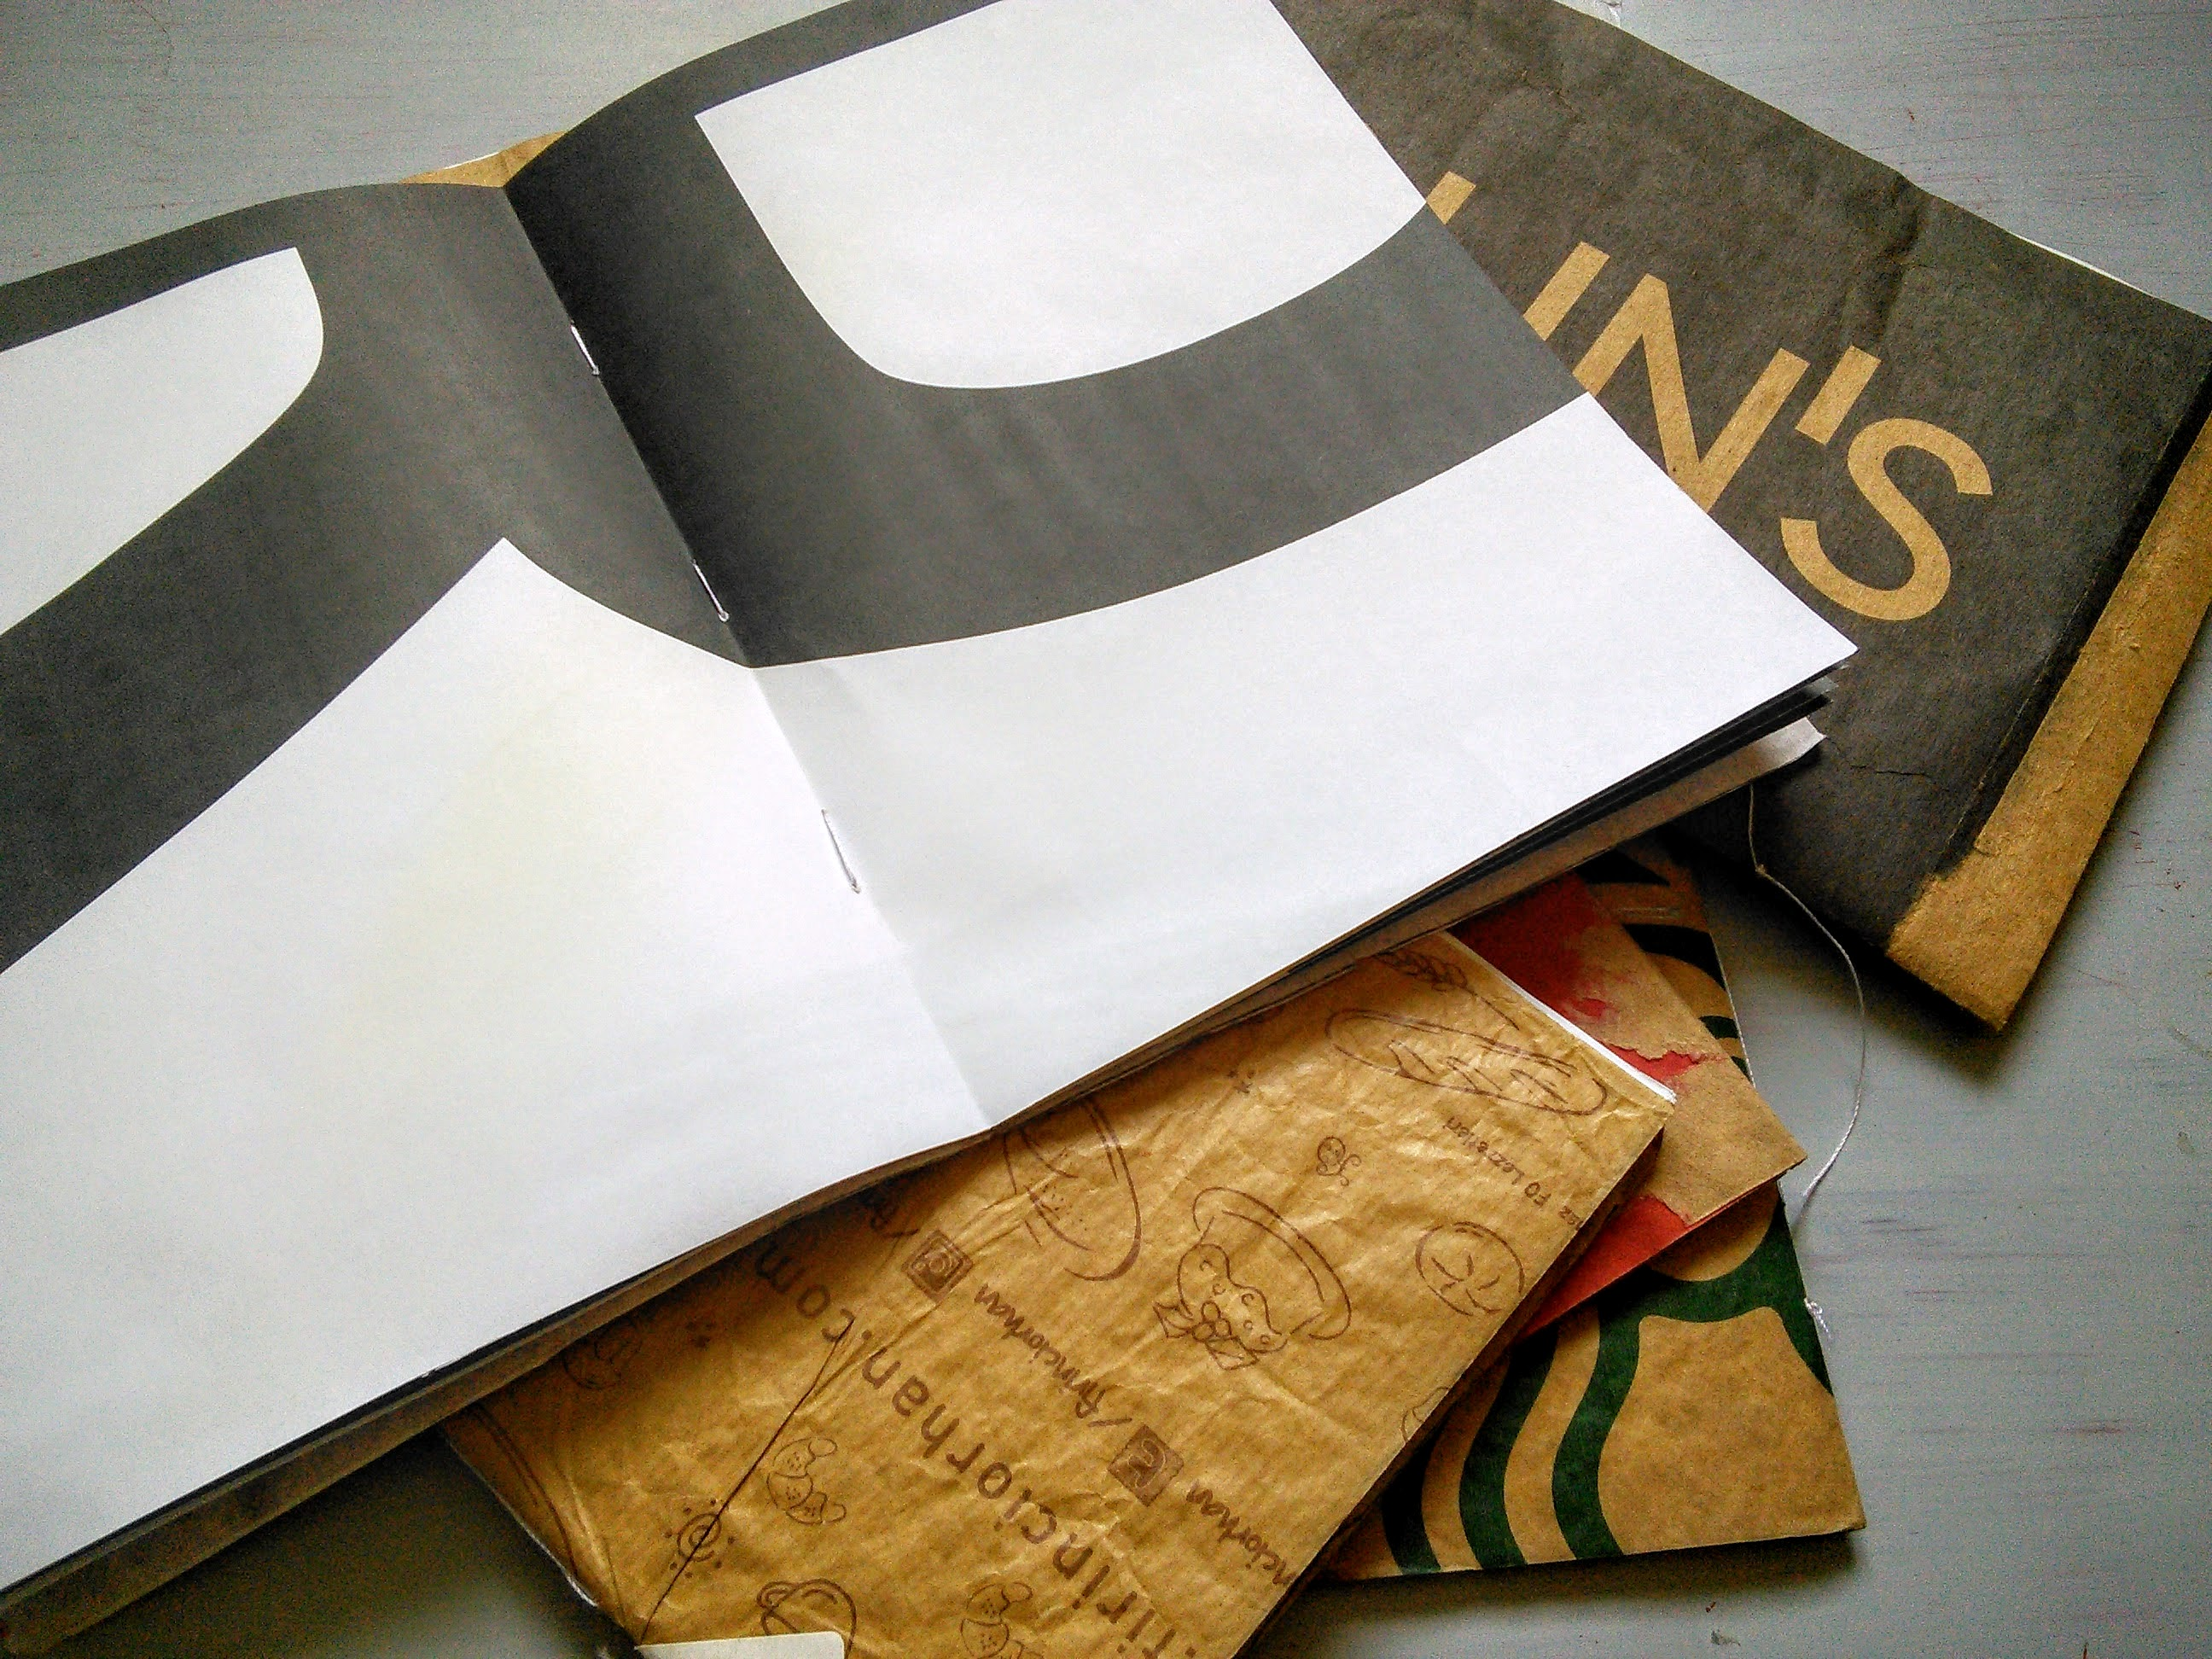
\includegraphics[height=10cm]{project_graphics/notebooks_puzzle_open.jpg}
  \caption{Notebooks, Puzzle series}
  \label{fig:CollectedAllTogether}
\end{figure}



\begin{figure}[!tbp]
  \centering
  \begin{minipage}[b]{0.48\textwidth}
    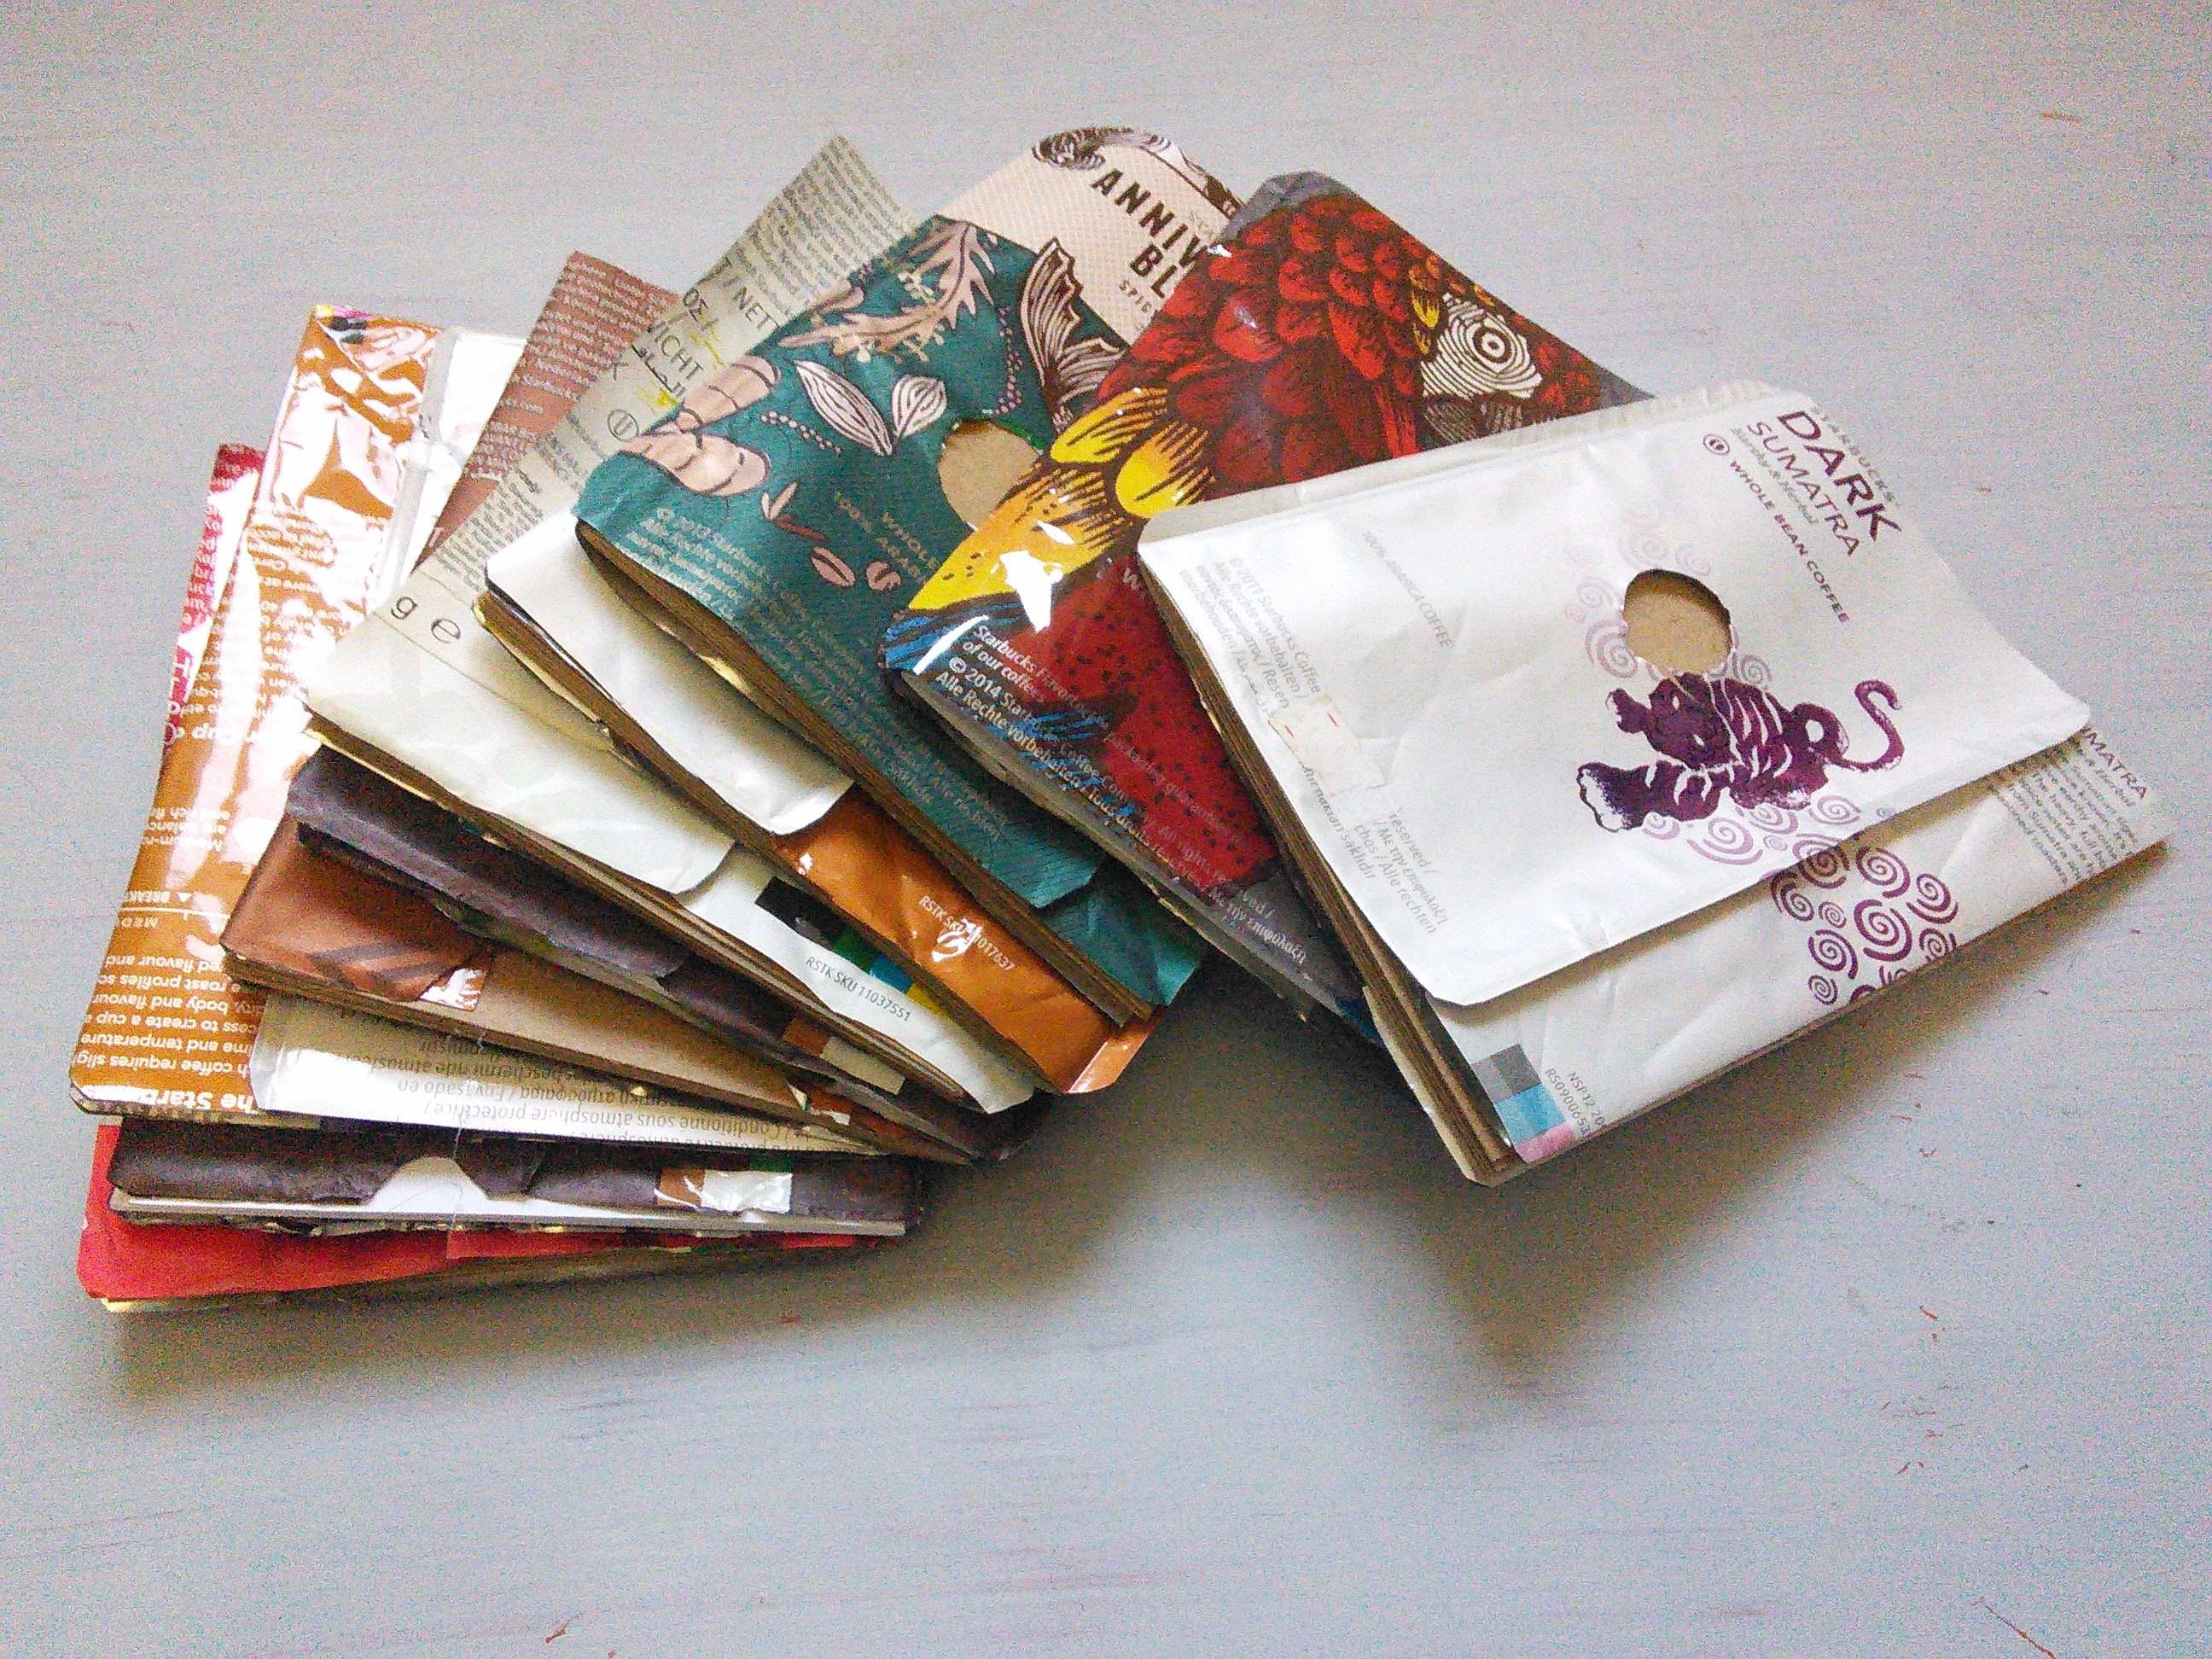
\includegraphics[width=\textwidth]{project_graphics/notebooks1.jpg}
    \caption{Notebooks, Reunion series}
    \label{fig:Notebooks1}
  \end{minipage}
  \hfill
  \begin{minipage}[b]{0.48\textwidth}
    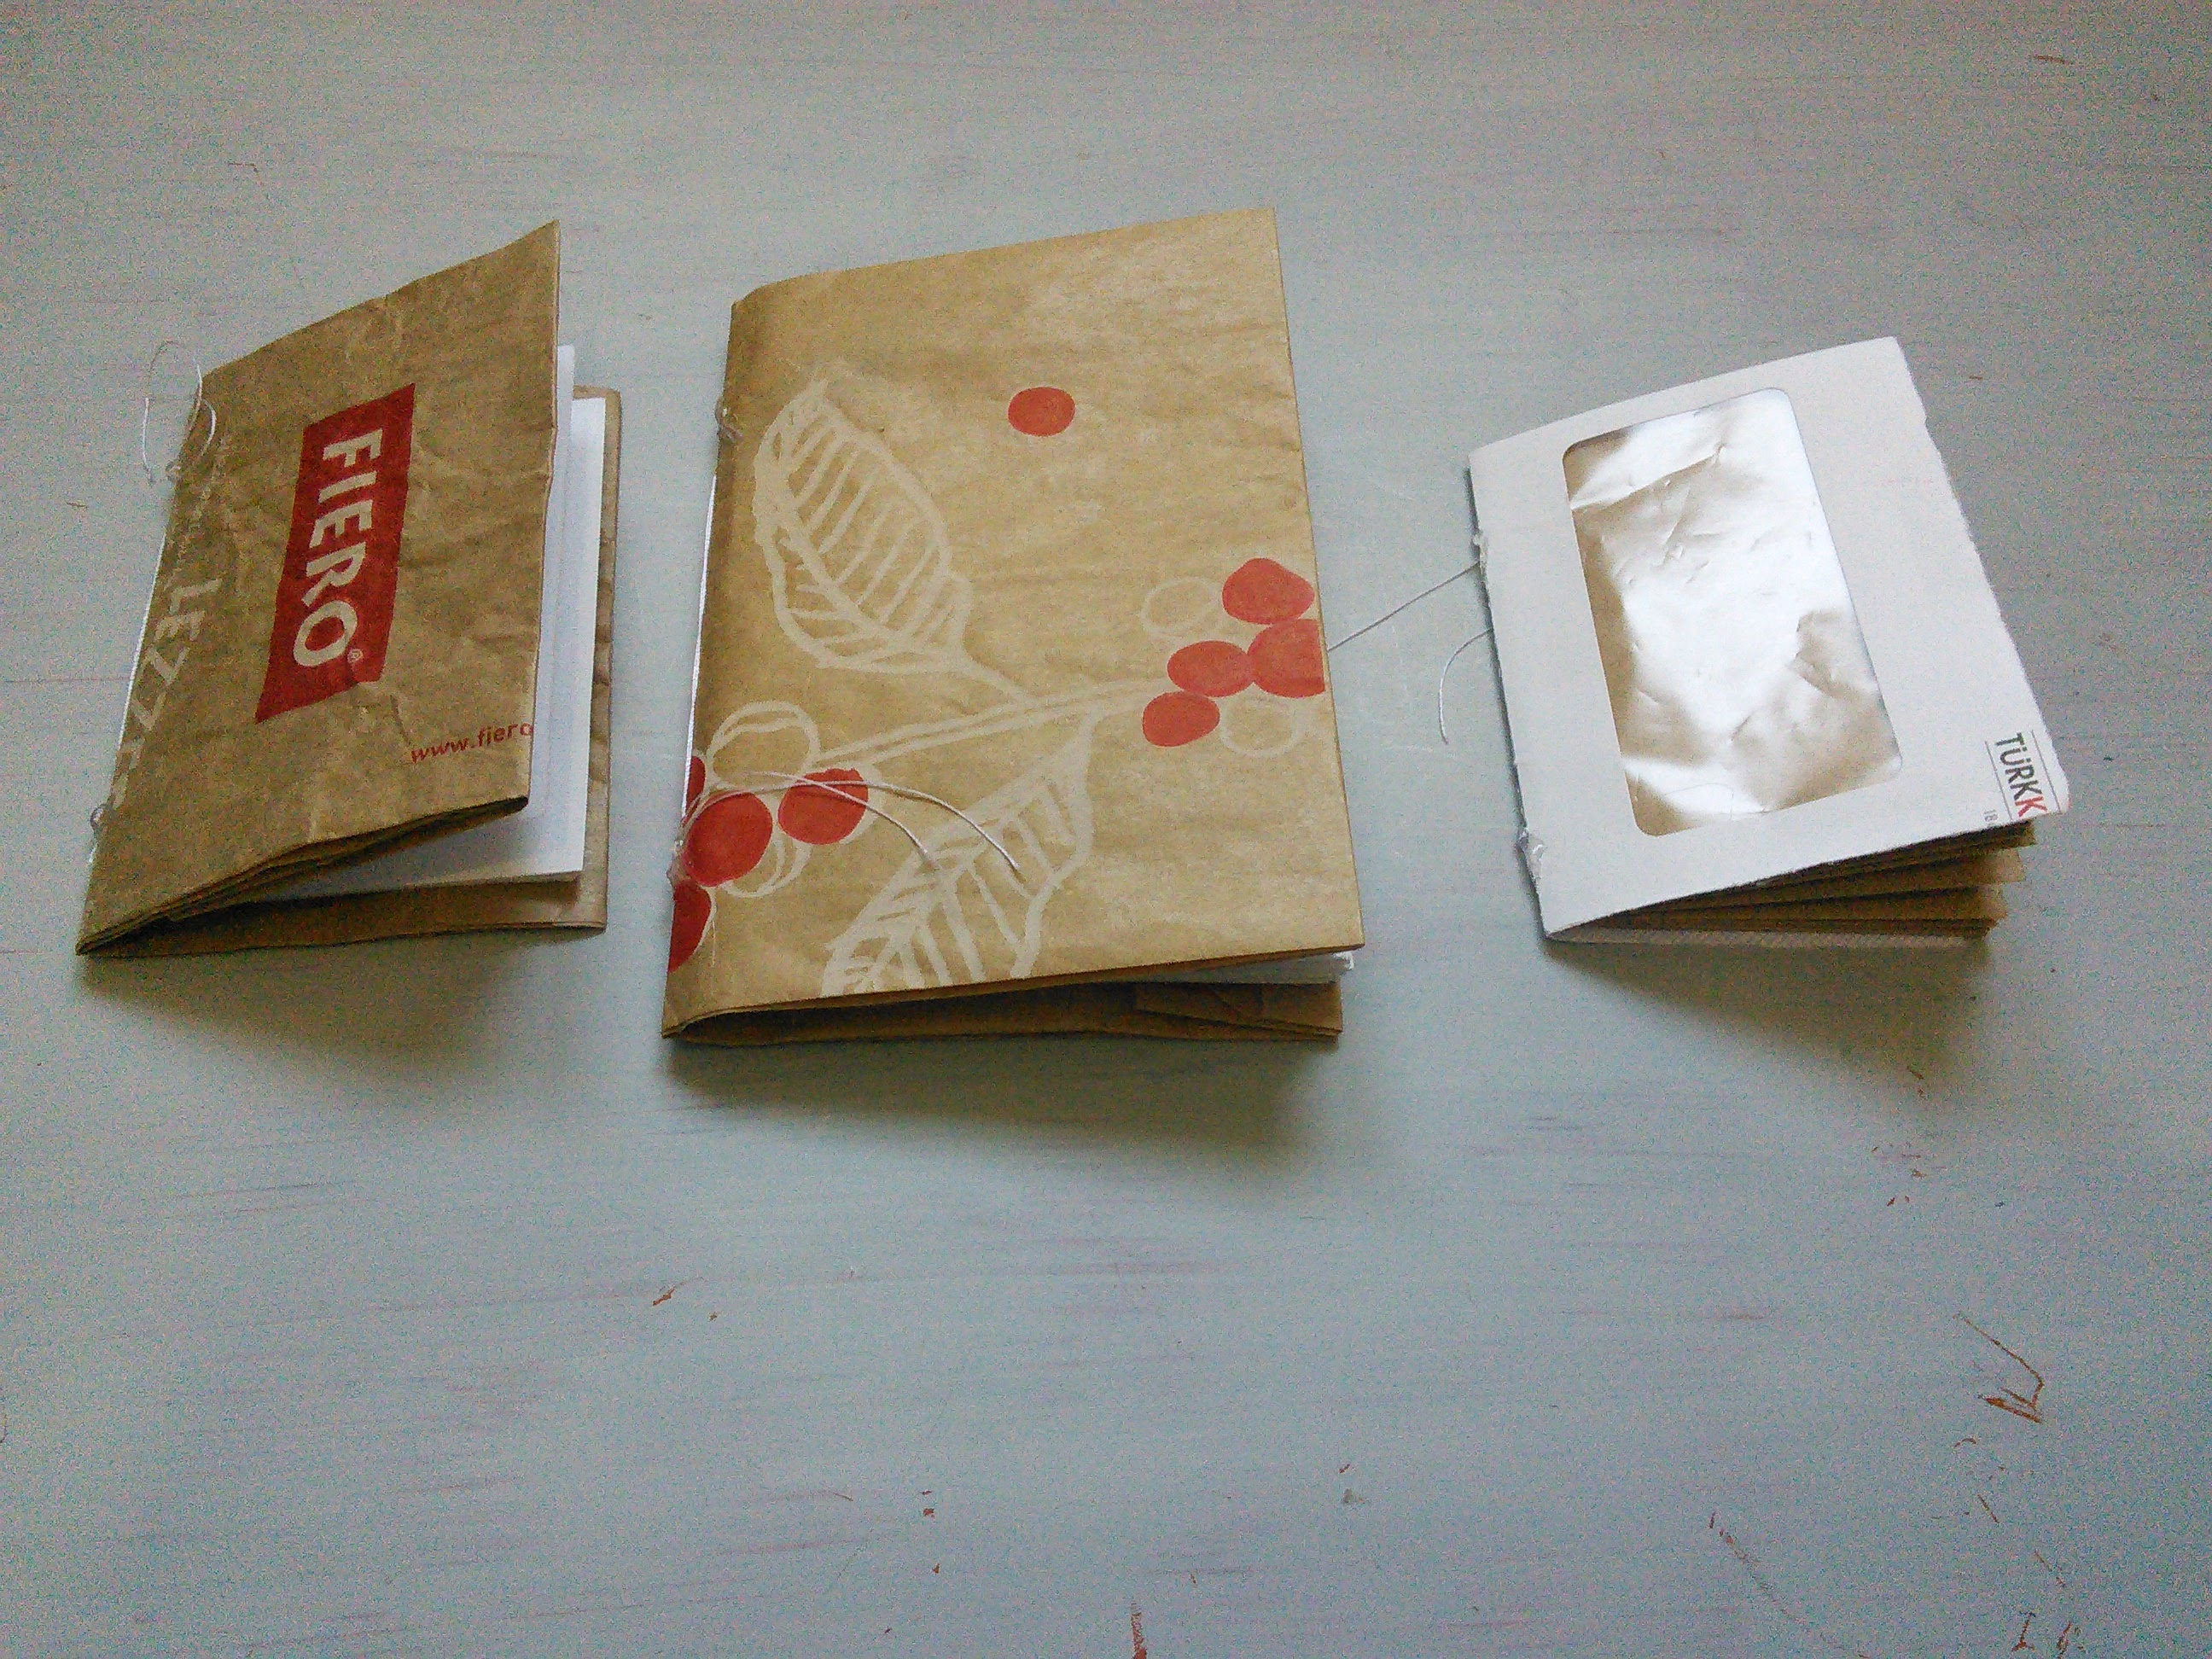
\includegraphics[width=\textwidth]{project_graphics/notebooks2.jpg}
    \caption{Notebooks, Secondhand series}
    \label{fig:Notebooks2}
  \end{minipage}
\end{figure}
%........................................


\end{document}